%% ATEF-DT -- revised manuscript.
%% Every run-dependent number is read from values.tex and every result table
%% from tables/*.tex; both are generated by experiments/make_values.py.
\documentclass[final,5p,times]{elsarticle}
\usepackage{amsmath,amssymb,amsthm}
\usepackage{graphicx}
\usepackage{booktabs}
\usepackage{multirow}
\usepackage{algorithm}
\usepackage{algorithmic}
\usepackage{url}
\usepackage{xcolor}
\usepackage{array}
\usepackage{tabularx}
\usepackage[hidelinks]{hyperref}
\usepackage{placeins}
%% float placement: keep figures and tables close to the text that discusses them
\renewcommand{\topfraction}{0.9}\renewcommand{\bottomfraction}{0.8}
\renewcommand{\textfraction}{0.07}\renewcommand{\floatpagefraction}{0.8}
\renewcommand{\dbltopfraction}{0.9}\renewcommand{\dblfloatpagefraction}{0.8}
\setcounter{topnumber}{3}\setcounter{bottomnumber}{2}\setcounter{totalnumber}{5}\setcounter{dbltopnumber}{3}
\setlength{\emergencystretch}{3em}
%% Float placement: the article has many tables, so let pages take more of them.
\setcounter{topnumber}{4}\setcounter{dbltopnumber}{4}\setcounter{totalnumber}{6}
\renewcommand{\topfraction}{0.95}\renewcommand{\dbltopfraction}{0.95}
\renewcommand{\textfraction}{0.05}\renewcommand{\floatpagefraction}{0.85}\renewcommand{\dblfloatpagefraction}{0.85}
\biboptions{sort&compress}
\journal{J. King Saud Univ. -- Comput. Inf. Sci.}

%% -- Revision marks ---------------------------------------------------
%% \showrevtrue : passages that answer a comment are coloured by the source of
%%                the first comment in their tag (blue E, red R1, green R2).
%% \showrevfalse: clean version.
\newif\ifshowrev
\showrevtrue
\definecolor{revE}{RGB}{0,70,170}      % Editor
\definecolor{revRone}{RGB}{185,20,20}  % Reviewer 1
\definecolor{revRtwo}{RGB}{0,115,55}   % Reviewer 2
\colorlet{revcur}{revE}
\ExplSyntaxOn
\bool_new:N \g__atef_first_bool
\cs_new_protected:Npn \__atef_tag:n #1
  {
    \str_if_eq:eeTF { \str_head:n {#1} } { E }
      { \tl_set:Nn \l_tmpa_tl { revE } }
      {
        \str_if_eq:eeTF { \str_range:nnn {#1} {1} {2} } { R1 }
          { \tl_set:Nn \l_tmpa_tl { revRone } }
          { \tl_set:Nn \l_tmpa_tl { revRtwo } }
      }
    \bool_if:NT \g__atef_first_bool { \tl_gset_eq:NN \g_tmpa_tl \l_tmpa_tl }
    \bool_gset_false:N \g__atef_first_bool
  }
% \rtag{E1, R1.1}: records the comments a passage answers (not printed) and
% colours the following \rev text by the source of the first comment.
\NewDocumentCommand{\rtag}{m}
  {
    \ifshowrev
      \bool_gset_true:N \g__atef_first_bool
      \clist_map_inline:nn {#1} { \__atef_tag:n {##1} }
      \colorlet{revcur}{\g_tmpa_tl}
    \fi
  }
\ExplSyntaxOff
% \revcap{tags}{text}: caption of a new or redrawn figure or table
\newcommand{\revcap}[2]{\caption{\rtag{#1}\rev{#2}}}
\newcommand{\rev}[1]{\ifshowrev{\color{revcur}#1}\else#1\fi}
\newenvironment{revblock}{\ifshowrev\color{revcur}\fi}{}

%% -- Run-dependent values ---------------------------------------------
\makeatletter
\newcommand{\defval}[2]{\expandafter\gdef\csname atefv@#1\endcsname{#2}}
\newcommand{\V}[1]{\@ifundefined{atefv@#1}{\PackageError{atefdt}{Value `#1' is not defined in values.tex}{Run experiments/make_values.py.}}{\csname atefv@#1\endcsname}}
\makeatother
\newcommand{\Vpm}[2]{\V{#1}\,$\pm$\,\V{#2}}
\makeatletter\newcommand{\tabin}[1]{\@@input tables/#1.tex }\makeatother  % expandable input for table bodies
% Generated by experiments/make_values.py -- do not edit by hand.
% 788 values from results/ (5 seeds).
\defval{E-atef}{17.72}
\defval{E-atef-a6}{17.72}
\defval{E-atef-a7}{2.28}
\defval{E-atef-a8}{0.62}
\defval{E-atef-a9}{0.45}
\defval{E-eafl}{11.28}
\defval{E-eafl-a6}{11.28}
\defval{E-eafl-a7}{2.66}
\defval{E-eafl-a8}{1.53}
\defval{E-eafl-a9}{1.37}
\defval{E-efair}{19.27}
\defval{E-eftrust}{19.25}
\defval{E-etrust}{11.66}
\defval{E-ffcs}{21.63}
\defval{E-full}{52.14}
\defval{E-lf00}{10.79}
\defval{E-lf05}{13.04}
\defval{E-lf10}{14.92}
\defval{E-lf15}{16.07}
\defval{E-lf20}{16.84}
\defval{E-lf30}{17.72}
\defval{E-lf40}{18.28}
\defval{E-rand}{21.30}
\defval{Ecomp-atef}{17.27}
\defval{Ecomp-eafl}{9.26}
\defval{Ecomp-efair}{17.38}
\defval{Ecomp-eftrust}{17.39}
\defval{Ecomp-etrust}{9.68}
\defval{Ecomp-ffcs}{19.56}
\defval{Ecomp-full}{47.11}
\defval{Ecomp-rand}{19.20}
\defval{Ecomp-sav-rand}{1.93}
\defval{Edl-atef}{0.18}
\defval{Edl-eafl}{0.18}
\defval{Edl-efair}{0.17}
\defval{Edl-eftrust}{0.17}
\defval{Edl-etrust}{0.18}
\defval{Edl-ffcs}{0.18}
\defval{Edl-full}{0.44}
\defval{Edl-rand}{0.18}
\defval{Esd-atef}{1.03}
\defval{Esd-eafl}{1.53}
\defval{Esd-efair}{1.03}
\defval{Esd-eftrust}{1.14}
\defval{Esd-etrust}{1.43}
\defval{Esd-ffcs}{1.46}
\defval{Esd-full}{3.80}
\defval{Esd-rand}{1.56}
\defval{Esig-atef}{0.011}
\defval{Esig-eafl}{0.011}
\defval{Esig-efair}{0.011}
\defval{Esig-eftrust}{0.011}
\defval{Esig-etrust}{0.011}
\defval{Esig-ffcs}{0.000}
\defval{Esig-full}{0.000}
\defval{Esig-rand}{0.000}
\defval{Eul-atef}{0.25}
\defval{Eul-eafl}{1.83}
\defval{Eul-efair}{1.71}
\defval{Eul-eftrust}{1.67}
\defval{Eul-etrust}{1.79}
\defval{Eul-ffcs}{1.89}
\defval{Eul-full}{4.59}
\defval{Eul-q16}{0.896}
\defval{Eul-q8}{0.463}
\defval{Eul-qglobal}{0.283}
\defval{Eul-rand}{1.92}
\defval{Eul-sav-rand}{1.67}
\defval{acc-atef}{96.67}
\defval{acc-eafl}{95.26}
\defval{acc-efair}{96.84}
\defval{acc-eftrust}{96.14}
\defval{acc-etrust}{95.79}
\defval{acc-ffcs}{97.54}
\defval{acc-full}{97.02}
\defval{acc-lf00}{96.32}
\defval{acc-lf05}{96.32}
\defval{acc-lf10}{95.96}
\defval{acc-lf15}{96.67}
\defval{acc-lf20}{96.67}
\defval{acc-lf30}{96.67}
\defval{acc-lf40}{97.37}
\defval{acc-q16}{97.02}
\defval{acc-q8}{96.67}
\defval{acc-qglobal}{96.67}
\defval{acc-rand}{97.37}
\defval{accgap-full}{0.35}
\defval{accgap-rand}{0.70}
\defval{acchigh-atef}{97.1}
\defval{acchigh-eafl}{96.3}
\defval{acchigh-efair}{97.1}
\defval{acchigh-eftrust}{96.3}
\defval{acchigh-etrust}{95.9}
\defval{acchigh-ffcs}{97.8}
\defval{acchigh-full}{97.6}
\defval{acchigh-rand}{97.6}
\defval{acclow-atef}{95.8}
\defval{acclow-eafl}{92.3}
\defval{acclow-efair}{96.4}
\defval{acclow-eftrust}{95.8}
\defval{acclow-etrust}{95.7}
\defval{acclow-ffcs}{97.0}
\defval{acclow-full}{95.8}
\defval{acclow-rand}{97.1}
\defval{accsd-atef}{0.73}
\defval{accsd-eafl}{1.82}
\defval{accsd-efair}{0.48}
\defval{accsd-eftrust}{1.00}
\defval{accsd-etrust}{0.73}
\defval{accsd-ffcs}{2.00}
\defval{accsd-full}{1.00}
\defval{accsd-rand}{1.07}
\defval{asr-clean}{0.5}
\defval{asr20-gm}{26}
\defval{asr20-mkrum}{56}
\defval{asr20-norep}{44}
\defval{asr20-rand}{89}
\defval{attackstart}{10}
\defval{below-main}{0}
\defval{cbound-atef}{0.570}
\defval{cbound-eafl}{1.401}
\defval{cbound-efair}{0.138}
\defval{cbound-eftrust}{0.567}
\defval{cbound-etrust}{1.512}
\defval{cbound-ffcs}{0.299}
\defval{cbound-full}{0.023}
\defval{cbound-lf00}{1.333}
\defval{cbound-lf05}{0.880}
\defval{cbound-lf10}{0.719}
\defval{cbound-lf15}{0.635}
\defval{cbound-lf20}{0.594}
\defval{cbound-lf30}{0.570}
\defval{cbound-lf40}{0.540}
\defval{cbound-rand}{0.104}
\defval{cl-cwmed}{97.0}
\defval{cl-gm}{96.8}
\defval{cl-mkrum}{96.8}
\defval{cl-norep}{97.0}
\defval{cl-norepgm}{96.8}
\defval{cl-trimmed}{97.0}
\defval{compr}{7.2}
\defval{compr-formula}{7.2}
\defval{compshare-a6}{90.3}
\defval{compshare-a7}{48.3}
\defval{compshare-a8}{8.6}
\defval{compshare-a9}{0.9}
\defval{compshare-atef}{97.5}
\defval{compshare-full}{90.3}
\defval{cpart-atef}{0.083}
\defval{cpart-eafl}{0.160}
\defval{cpart-efair}{0.018}
\defval{cpart-eftrust}{0.086}
\defval{cpart-etrust}{0.172}
\defval{cpart-ffcs}{0.047}
\defval{cpart-full}{0.005}
\defval{cpart-lf00}{0.157}
\defval{cpart-lf05}{0.116}
\defval{cpart-lf10}{0.102}
\defval{cpart-lf15}{0.087}
\defval{cpart-lf20}{0.080}
\defval{cpart-lf30}{0.083}
\defval{cpart-lf40}{0.080}
\defval{cpart-rand}{0.013}
\defval{d}{2049}
\defval{downMb-atef}{26.2}
\defval{downMb-eafl}{26.2}
\defval{downMb-efair}{26.2}
\defval{downMb-eftrust}{26.2}
\defval{downMb-etrust}{26.2}
\defval{downMb-ffcs}{26.2}
\defval{downMb-full}{63.6}
\defval{downMb-rand}{26.2}
\defval{extra-eafl}{57.1}
\defval{fe-clean}{2.0}
\defval{g-acc-ad10}{96.7}
\defval{g-acc-ad20}{96.5}
\defval{g-acc-ad30}{97.0}
\defval{g-acc-ad40}{96.1}
\defval{g-acc-bd10}{96.1}
\defval{g-acc-bd20}{95.4}
\defval{g-acc-bd30}{95.3}
\defval{g-acc-bd40}{94.4}
\defval{g-acc-ga10}{96.3}
\defval{g-acc-ga20}{96.7}
\defval{g-acc-ga30}{97.0}
\defval{g-acc-ga40}{96.3}
\defval{g-acc-lf10}{96.7}
\defval{g-acc-lf20}{95.6}
\defval{g-acc-lf30}{95.6}
\defval{g-acc-lf40}{65.8}
\defval{g-acc-sc10}{96.8}
\defval{g-acc-sc20}{96.8}
\defval{g-acc-sc30}{96.8}
\defval{g-acc-sc40}{96.5}
\defval{g-acc-sf10}{96.3}
\defval{g-acc-sf20}{96.3}
\defval{g-acc-sf30}{90.9}
\defval{g-acc-sf40}{63.5}
\defval{g-accsd-ad10}{0.7}
\defval{g-accsd-ad20}{0.9}
\defval{g-accsd-ad30}{1.3}
\defval{g-accsd-ad40}{1.2}
\defval{g-accsd-bd10}{0.8}
\defval{g-accsd-bd20}{1.4}
\defval{g-accsd-bd30}{1.0}
\defval{g-accsd-bd40}{1.2}
\defval{g-accsd-ga10}{1.1}
\defval{g-accsd-ga20}{0.4}
\defval{g-accsd-ga30}{0.8}
\defval{g-accsd-ga40}{1.1}
\defval{g-accsd-lf10}{0.7}
\defval{g-accsd-lf20}{1.2}
\defval{g-accsd-lf30}{0.6}
\defval{g-accsd-lf40}{22.1}
\defval{g-accsd-sc10}{0.8}
\defval{g-accsd-sc20}{1.0}
\defval{g-accsd-sc30}{0.5}
\defval{g-accsd-sc40}{0.6}
\defval{g-accsd-sf10}{0.7}
\defval{g-accsd-sf20}{0.7}
\defval{g-accsd-sf30}{10.2}
\defval{g-accsd-sf40}{41.6}
\defval{g-asr-bd10}{5}
\defval{g-asr-bd20}{51}
\defval{g-asr-bd30}{74}
\defval{g-asr-bd40}{89}
\defval{g-bar-ad10}{0}
\defval{g-bar-ad20}{0}
\defval{g-bar-ad30}{0}
\defval{g-bar-ad40}{0}
\defval{g-bar-bd10}{1}
\defval{g-bar-bd20}{0}
\defval{g-bar-bd30}{1}
\defval{g-bar-bd40}{6}
\defval{g-bar-ga10}{0}
\defval{g-bar-ga20}{0}
\defval{g-bar-ga30}{0}
\defval{g-bar-ga40}{0}
\defval{g-bar-lf10}{6}
\defval{g-bar-lf20}{5}
\defval{g-bar-lf30}{11}
\defval{g-bar-lf40}{1}
\defval{g-bar-sc10}{0}
\defval{g-bar-sc20}{1}
\defval{g-bar-sc30}{0}
\defval{g-bar-sc40}{1}
\defval{g-bar-sf10}{0}
\defval{g-bar-sf20}{4}
\defval{g-bar-sf30}{3}
\defval{g-bar-sf40}{2}
\defval{g-fe-ad10}{2.2}
\defval{g-fe-ad20}{3.8}
\defval{g-fe-ad30}{14.3}
\defval{g-fe-ad40}{26.7}
\defval{g-fe-bd10}{2.2}
\defval{g-fe-bd20}{2.5}
\defval{g-fe-bd30}{2.9}
\defval{g-fe-bd40}{1.7}
\defval{g-fe-ga10}{1.1}
\defval{g-fe-ga20}{3.8}
\defval{g-fe-ga30}{0.0}
\defval{g-fe-ga40}{1.7}
\defval{g-fe-lf10}{5.6}
\defval{g-fe-lf20}{1.2}
\defval{g-fe-lf30}{0.0}
\defval{g-fe-lf40}{1.7}
\defval{g-fe-sc10}{4.4}
\defval{g-fe-sc20}{1.2}
\defval{g-fe-sc30}{1.4}
\defval{g-fe-sc40}{0.0}
\defval{g-fe-sf10}{2.2}
\defval{g-fe-sf20}{1.2}
\defval{g-fe-sf30}{0.0}
\defval{g-fe-sf40}{16.7}
\defval{g-malsel-ad10}{10.1}
\defval{g-malsel-ad20}{24.1}
\defval{g-malsel-ad30}{38.6}
\defval{g-malsel-ad40}{49.9}
\defval{g-malsel-bd10}{9.1}
\defval{g-malsel-bd20}{21.2}
\defval{g-malsel-bd30}{29.7}
\defval{g-malsel-bd40}{38.0}
\defval{g-malsel-ga10}{9.4}
\defval{g-malsel-ga20}{20.8}
\defval{g-malsel-ga30}{30.2}
\defval{g-malsel-ga40}{38.8}
\defval{g-malsel-lf10}{7.2}
\defval{g-malsel-lf20}{19.6}
\defval{g-malsel-lf30}{25.8}
\defval{g-malsel-lf40}{38.7}
\defval{g-malsel-sc10}{9.6}
\defval{g-malsel-sc20}{20.1}
\defval{g-malsel-sc30}{30.6}
\defval{g-malsel-sc40}{38.8}
\defval{g-malsel-sf10}{9.4}
\defval{g-malsel-sf20}{19.4}
\defval{g-malsel-sf30}{29.0}
\defval{g-malsel-sf40}{41.7}
\defval{g-malw-ad10}{15.1}
\defval{g-malw-ad20}{45.6}
\defval{g-malw-ad30}{72.0}
\defval{g-malw-ad40}{83.7}
\defval{g-malw-bd10}{0.1}
\defval{g-malw-bd20}{9.7}
\defval{g-malw-bd30}{21.1}
\defval{g-malw-bd40}{26.5}
\defval{g-malw-ga10}{3.3}
\defval{g-malw-ga20}{10.5}
\defval{g-malw-ga30}{19.1}
\defval{g-malw-ga40}{25.2}
\defval{g-malw-lf10}{0.2}
\defval{g-malw-lf20}{1.3}
\defval{g-malw-lf30}{6.8}
\defval{g-malw-lf40}{24.3}
\defval{g-malw-sc10}{2.3}
\defval{g-malw-sc20}{11.2}
\defval{g-malw-sc30}{21.5}
\defval{g-malw-sc40}{27.6}
\defval{g-malw-sf10}{4.2}
\defval{g-malw-sf20}{10.8}
\defval{g-malw-sf30}{19.5}
\defval{g-malw-sf40}{35.9}
\defval{g-nadv-ad10}{10}
\defval{g-nadv-ad20}{20}
\defval{g-nadv-ad30}{30}
\defval{g-nadv-ad40}{40}
\defval{g-nadv-bd10}{10}
\defval{g-nadv-bd20}{20}
\defval{g-nadv-bd30}{30}
\defval{g-nadv-bd40}{40}
\defval{g-nadv-ga10}{10}
\defval{g-nadv-ga20}{20}
\defval{g-nadv-ga30}{30}
\defval{g-nadv-ga40}{40}
\defval{g-nadv-lf10}{10}
\defval{g-nadv-lf20}{20}
\defval{g-nadv-lf30}{30}
\defval{g-nadv-lf40}{40}
\defval{g-nadv-sc10}{10}
\defval{g-nadv-sc20}{20}
\defval{g-nadv-sc30}{30}
\defval{g-nadv-sc40}{40}
\defval{g-nadv-sf10}{10}
\defval{g-nadv-sf20}{20}
\defval{g-nadv-sf30}{30}
\defval{g-nadv-sf40}{40}
\defval{g-rej-ad10}{0.0}
\defval{g-rej-ad20}{0.0}
\defval{g-rej-ad30}{0.0}
\defval{g-rej-ad40}{0.0}
\defval{g-rej-bd10}{0.7}
\defval{g-rej-bd20}{0.0}
\defval{g-rej-bd30}{0.2}
\defval{g-rej-bd40}{1.0}
\defval{g-rej-ga10}{0.0}
\defval{g-rej-ga20}{0.0}
\defval{g-rej-ga30}{0.0}
\defval{g-rej-ga40}{0.0}
\defval{g-rej-lf10}{7.2}
\defval{g-rej-lf20}{1.7}
\defval{g-rej-lf30}{2.8}
\defval{g-rej-lf40}{0.2}
\defval{g-rej-sc10}{0.0}
\defval{g-rej-sc20}{0.3}
\defval{g-rej-sc30}{0.0}
\defval{g-rej-sc40}{0.2}
\defval{g-rej-sf10}{0.0}
\defval{g-rej-sf20}{1.4}
\defval{g-rej-sf30}{0.7}
\defval{g-rej-sf40}{0.3}
\defval{g-viol-ad10}{0.0}
\defval{g-viol-ad20}{6.5}
\defval{g-viol-ad30}{37.0}
\defval{g-viol-ad40}{66.0}
\defval{g-viol-bd10}{0.0}
\defval{g-viol-bd20}{1.5}
\defval{g-viol-bd30}{14.0}
\defval{g-viol-bd40}{34.5}
\defval{g-viol-ga10}{0.0}
\defval{g-viol-ga20}{2.0}
\defval{g-viol-ga30}{13.5}
\defval{g-viol-ga40}{36.5}
\defval{g-viol-lf10}{0.0}
\defval{g-viol-lf20}{1.0}
\defval{g-viol-lf30}{10.5}
\defval{g-viol-lf40}{34.0}
\defval{g-viol-sc10}{0.0}
\defval{g-viol-sc20}{2.0}
\defval{g-viol-sc30}{13.0}
\defval{g-viol-sc40}{33.0}
\defval{g-viol-sf10}{0.0}
\defval{g-viol-sf20}{2.0}
\defval{g-viol-sf30}{11.0}
\defval{g-viol-sf40}{45.0}
\defval{hi-lf30-dt}{95.6}
\defval{hi-lf30-gm}{93.3}
\defval{hi-lf30-mkrum}{88.1}
\defval{hi-lf30-norep}{91.2}
\defval{hi-lf30-random}{72.3}
\defval{hi-lf40-dt}{65.8}
\defval{hi-lf40-gm}{76.8}
\defval{hi-lf40-mkrum}{81.2}
\defval{hi-lf40-norep}{76.7}
\defval{hi-lf40-random}{50.0}
\defval{hi-sf30-dt}{90.9}
\defval{hi-sf30-gm}{94.6}
\defval{hi-sf30-mkrum}{95.8}
\defval{hi-sf30-norep}{94.9}
\defval{hi-sf30-random}{87.2}
\defval{hi-sf40-dt}{63.5}
\defval{hi-sf40-gm}{93.5}
\defval{hi-sf40-mkrum}{86.3}
\defval{hi-sf40-norep}{93.2}
\defval{hi-sf40-random}{64.4}
\defval{jain-atef}{0.968}
\defval{jain-atef-a6}{0.968}
\defval{jain-atef-a7}{0.993}
\defval{jain-atef-a8}{0.991}
\defval{jain-atef-a9}{0.995}
\defval{jain-eafl}{0.441}
\defval{jain-eafl-a6}{0.441}
\defval{jain-eafl-a7}{0.548}
\defval{jain-eafl-a8}{0.673}
\defval{jain-eafl-a9}{0.704}
\defval{jain-efair}{0.974}
\defval{jain-eftrust}{0.965}
\defval{jain-etrust}{0.466}
\defval{jain-ffcs}{0.835}
\defval{jain-full}{0.995}
\defval{jain-lf00}{0.501}
\defval{jain-lf05}{0.701}
\defval{jain-lf10}{0.831}
\defval{jain-lf15}{0.905}
\defval{jain-lf20}{0.937}
\defval{jain-lf30}{0.968}
\defval{jain-lf40}{0.980}
\defval{jain-rand}{0.963}
\defval{jain-req}{0.95}
\defval{jainexp}{0.971}
\defval{jainsd-atef}{0.004}
\defval{jainsd-eafl}{0.010}
\defval{jainsd-efair}{0.004}
\defval{jainsd-eftrust}{0.009}
\defval{jainsd-etrust}{0.032}
\defval{jainsd-ffcs}{0.052}
\defval{jainsd-full}{0.007}
\defval{jainsd-rand}{0.015}
\defval{kstar}{6}
\defval{lambdaF}{3.0}
\defval{lf20-atef}{95.6}
\defval{lf20-cwmed}{95.3}
\defval{lf20-eafl}{81.2}
\defval{lf20-efair}{90.7}
\defval{lf20-eftrust}{96.5}
\defval{lf20-etrust}{91.8}
\defval{lf20-ffcs}{94.2}
\defval{lf20-full}{88.6}
\defval{lf20-gm}{96.8}
\defval{lf20-mkrum}{95.6}
\defval{lf20-norep}{95.8}
\defval{lf20-norepgm}{96.0}
\defval{lf20-rand}{81.9}
\defval{lf20-trimmed}{88.9}
\defval{lf20sd-atef}{1.2}
\defval{lf20sd-eafl}{8.7}
\defval{lf20sd-efair}{7.1}
\defval{lf20sd-etrust}{9.6}
\defval{lf20sd-ffcs}{1.6}
\defval{lf20sd-full}{3.5}
\defval{lf20sd-rand}{10.0}
\defval{loss-atef}{0.083}
\defval{loss-full}{0.065}
\defval{lr}{1.0}
\defval{lrval-01}{0.1223}
\defval{lrval-02}{0.1020}
\defval{lrval-05}{0.0876}
\defval{lrval-10}{0.0824}
\defval{meanb}{4.41}
\defval{meanb-q16}{16.00}
\defval{meanb-q8}{8.00}
\defval{meanb-qglobal}{4.80}
\defval{metaMb}{0.026}
\defval{npmax}{118}
\defval{npmin}{6}
\defval{nseeds}{five}
\defval{ntest}{114}
\defval{ntrain}{409}
\defval{nval}{46}
\defval{on0-lf-acc}{95.3}
\defval{on0-lf-bar}{7}
\defval{on0-lf-malw}{1.6}
\defval{on0-sf-acc}{94.9}
\defval{on0-sf-bar}{4}
\defval{on0-sf-malw}{8.0}
\defval{on10-lf-acc}{95.6}
\defval{on10-lf-bar}{5}
\defval{on10-lf-malw}{1.3}
\defval{on10-sf-acc}{96.3}
\defval{on10-sf-bar}{4}
\defval{on10-sf-malw}{10.8}
\defval{outage}{3.0}
\defval{p-E-atef-rand}{0.001}
\defval{p-acc-atef-rand}{0.10}
\defval{p-atef}{0.54}
\defval{p-eafl}{0.22}
\defval{p-efair}{0.75}
\defval{p-eftrust}{0.03}
\defval{p-etrust}{0.02}
\defval{p-ffcs}{0.30}
\defval{p-full}{1.00}
\defval{p-lf-atef-norep}{0.80}
\defval{p-lf-atef-rand}{0.05}
\defval{p-rand}{0.48}
\defval{p-sens-atef}{0.11}
\defval{payloadMb}{3.61}
\defval{pil1-atef}{0.79}
\defval{pil1-eafl}{1.49}
\defval{pil1-efair}{0.24}
\defval{pil1-eftrust}{0.79}
\defval{pil1-etrust}{1.54}
\defval{pil1-ffcs}{0.41}
\defval{pil1-full}{0.04}
\defval{pil1-lf00}{1.42}
\defval{pil1-lf05}{1.13}
\defval{pil1-lf10}{0.94}
\defval{pil1-lf15}{0.89}
\defval{pil1-lf20}{0.84}
\defval{pil1-lf30}{0.79}
\defval{pil1-lf40}{0.74}
\defval{pil1-rand}{0.15}
\defval{pmax}{500}
\defval{resc-add-01}{5.9}
\defval{resc-add-10}{45.5}
\defval{resc-prod-01}{0.0}
\defval{resc-prod-10}{0.0}
\defval{rescE-add-1}{19.18}
\defval{rescE-add-10}{12.82}
\defval{rescE-prod-1}{17.72}
\defval{rescE-prod-10}{17.72}
\defval{rescjain-add-1}{0.990}
\defval{rescjain-add-10}{0.756}
\defval{rescjain-prod-1}{0.968}
\defval{rescjain-prod-10}{0.968}
\defval{sav-eafl-full}{78.4}
\defval{sav-efair}{8.1}
\defval{sav-full}{66.0}
\defval{sav-full-a6}{66.0}
\defval{sav-full-a7}{76.6}
\defval{sav-full-a8}{88.8}
\defval{sav-full-a9}{91.2}
\defval{sav-full-eta02}{67.8}
\defval{sav-full-eta035}{66.0}
\defval{sav-full-eta05}{65.3}
\defval{sav-rand}{16.8}
\defval{sav-rand-a6}{16.8}
\defval{sav-rand-a7}{43.3}
\defval{sav-rand-a8}{73.2}
\defval{sav-rand-a9}{78.9}
\defval{sav-rand-eta02}{21.3}
\defval{sav-rand-eta035}{16.8}
\defval{sav-rand-eta05}{15.0}
\defval{sav-rand-full}{59.1}
\defval{sc-E-atef-100}{104}
\defval{sc-E-atef-20}{20}
\defval{sc-E-atef-200}{210}
\defval{sc-E-atef-50}{51}
\defval{sc-E-atef-500}{521}
\defval{sc-E-eafl-100}{80}
\defval{sc-E-eafl-20}{16}
\defval{sc-E-eafl-200}{159}
\defval{sc-E-eafl-50}{40}
\defval{sc-E-eafl-500}{391}
\defval{sc-E-ffcs-100}{115}
\defval{sc-E-ffcs-20}{23}
\defval{sc-E-ffcs-200}{230}
\defval{sc-E-ffcs-50}{58}
\defval{sc-E-ffcs-500}{570}
\defval{sc-E-full-100}{275}
\defval{sc-E-full-20}{54}
\defval{sc-E-full-200}{547}
\defval{sc-E-full-50}{137}
\defval{sc-E-full-500}{1361}
\defval{sc-E-rand-100}{115}
\defval{sc-E-rand-20}{22}
\defval{sc-E-rand-200}{230}
\defval{sc-E-rand-50}{57}
\defval{sc-E-rand-500}{570}
\defval{sc-acc-atef-100}{96.7}
\defval{sc-acc-atef-20}{96.5}
\defval{sc-acc-atef-200}{96.8}
\defval{sc-acc-atef-50}{96.7}
\defval{sc-acc-atef-500}{96.5}
\defval{sc-acc-eafl-100}{97.2}
\defval{sc-acc-eafl-20}{94.6}
\defval{sc-acc-eafl-200}{97.2}
\defval{sc-acc-eafl-50}{97.0}
\defval{sc-acc-eafl-500}{96.8}
\defval{sc-acc-ffcs-100}{97.5}
\defval{sc-acc-ffcs-20}{97.5}
\defval{sc-acc-ffcs-200}{97.5}
\defval{sc-acc-ffcs-50}{97.5}
\defval{sc-acc-ffcs-500}{97.9}
\defval{sc-acc-full-100}{97.5}
\defval{sc-acc-full-20}{96.8}
\defval{sc-acc-full-200}{97.2}
\defval{sc-acc-full-50}{97.2}
\defval{sc-acc-full-500}{97.0}
\defval{sc-acc-rand-100}{97.5}
\defval{sc-acc-rand-20}{96.5}
\defval{sc-acc-rand-200}{97.0}
\defval{sc-acc-rand-50}{97.7}
\defval{sc-acc-rand-500}{97.0}
\defval{sc-jain-atef-100}{0.945}
\defval{sc-jain-atef-20}{0.977}
\defval{sc-jain-atef-200}{0.933}
\defval{sc-jain-atef-50}{0.955}
\defval{sc-jain-atef-500}{0.950}
\defval{sc-jain-eafl-100}{0.431}
\defval{sc-jain-eafl-20}{0.438}
\defval{sc-jain-eafl-200}{0.431}
\defval{sc-jain-eafl-50}{0.430}
\defval{sc-jain-eafl-500}{0.430}
\defval{sc-jain-ffcs-100}{0.776}
\defval{sc-jain-ffcs-20}{0.811}
\defval{sc-jain-ffcs-200}{0.751}
\defval{sc-jain-ffcs-50}{0.769}
\defval{sc-jain-ffcs-500}{0.741}
\defval{sc-jain-full-100}{0.988}
\defval{sc-jain-full-20}{0.995}
\defval{sc-jain-full-200}{0.979}
\defval{sc-jain-full-50}{0.985}
\defval{sc-jain-full-500}{0.987}
\defval{sc-jain-rand-100}{0.962}
\defval{sc-jain-rand-20}{0.963}
\defval{sc-jain-rand-200}{0.952}
\defval{sc-jain-rand-50}{0.959}
\defval{sc-jain-rand-500}{0.959}
\defval{sc-sav-full-100}{62.2}
\defval{sc-sav-full-20}{63.5}
\defval{sc-sav-full-200}{61.7}
\defval{sc-sav-full-50}{62.5}
\defval{sc-sav-full-500}{61.7}
\defval{sc-sav-rand-100}{9.6}
\defval{sc-sav-rand-20}{10.5}
\defval{sc-sav-rand-200}{9.0}
\defval{sc-sav-rand-50}{10.5}
\defval{sc-sav-rand-500}{8.5}
\defval{sched-E-add}{17.40}
\defval{sched-E-dpp}{17.75}
\defval{sched-E-prod}{17.43}
\defval{sched-E-seqef}{18.32}
\defval{sched-E-seqfe}{19.87}
\defval{sched-Esd-add}{1.21}
\defval{sched-Esd-dpp}{1.27}
\defval{sched-Esd-prod}{1.09}
\defval{sched-Esd-seqef}{1.49}
\defval{sched-Esd-seqfe}{1.37}
\defval{sched-J-add}{0.962}
\defval{sched-J-dpp}{0.955}
\defval{sched-J-prod}{0.956}
\defval{sched-J-seqef}{0.965}
\defval{sched-J-seqfe}{0.978}
\defval{sched-diff-add}{-0.02}
\defval{sched-diff-dpp}{0.32}
\defval{sched-diff-seqef}{0.89}
\defval{sched-diff-seqfe}{2.44}
\defval{sched-gap-add}{0.32}
\defval{sched-knob-add}{1}
\defval{sched-knob-dpp}{10}
\defval{sched-knob-prod}{2.5}
\defval{sched-knob-seqef}{18}
\defval{sched-knob-seqfe}{8}
\defval{sched-p-add}{0.907}
\defval{sched-p-dpp}{0.094}
\defval{sched-p-seqef}{0.128}
\defval{sched-p-seqfe}{0.001}
\defval{selhigh-atef}{43.1}
\defval{selhigh-eafl}{0.2}
\defval{selhigh-efair}{43.4}
\defval{selhigh-eftrust}{43.7}
\defval{selhigh-etrust}{1.8}
\defval{selhigh-ffcs}{50.5}
\defval{selhigh-full}{50.1}
\defval{selhigh-rand}{49.0}
\defval{sens-atef}{92.9}
\defval{sens-eafl}{93.3}
\defval{sens-efair}{95.7}
\defval{sens-eftrust}{91.9}
\defval{sens-etrust}{91.4}
\defval{sens-ffcs}{97.6}
\defval{sens-full}{95.7}
\defval{sens-rand}{95.7}
\defval{sensgap-full}{2.9}
\defval{sf20-atef}{96.3}
\defval{sf20-cwmed}{94.7}
\defval{sf20-eafl}{88.1}
\defval{sf20-efair}{94.6}
\defval{sf20-etrust}{94.7}
\defval{sf20-ffcs}{95.8}
\defval{sf20-full}{94.7}
\defval{sf20-gm}{94.9}
\defval{sf20-mkrum}{96.5}
\defval{sf20-norep}{96.0}
\defval{sf20-norepgm}{94.7}
\defval{sf20-rand}{92.8}
\defval{sf20-trimmed}{94.7}
\defval{smean}{0.82}
\defval{smin}{0.67}
\defval{spec-atef}{98.9}
\defval{spec-eafl}{96.4}
\defval{spec-efair}{97.5}
\defval{spec-eftrust}{98.6}
\defval{spec-etrust}{98.3}
\defval{spec-ffcs}{97.5}
\defval{spec-full}{97.8}
\defval{spec-rand}{98.3}
\defval{stateMb}{0.155}
\defval{t-gm-100}{2.5}
\defval{t-gm-20}{0.7}
\defval{t-gm-200}{6.7}
\defval{t-gm-50}{1.3}
\defval{t-gm-500}{16.5}
\defval{t-total-100}{2.9}
\defval{t-total-20}{0.9}
\defval{t-total-200}{7.5}
\defval{t-total-50}{1.5}
\defval{t-total-500}{18.4}
\defval{tot-red}{42.9}
\defval{totMb-atef}{30.0}
\defval{totMb-eftrust}{52.6}
\defval{tw-acc-instant}{96.7}
\defval{tw-acc-none}{97.2}
\defval{tw-acc-twin}{96.0}
\defval{tw-breach-ar}{5.4}
\defval{tw-breach-instant}{8.4}
\defval{tw-breach-none}{25.8}
\defval{tw-breach-twin}{3.8}
\defval{tw-dep-instant}{15.2}
\defval{tw-dep-none}{19.8}
\defval{tw-dep-twin}{13.4}
\defval{tw-jain-instant}{0.936}
\defval{tw-jain-none}{0.961}
\defval{tw-jain-twin}{0.916}
\defval{tw-mae-ar}{0.210}
\defval{tw-mae-ar-01}{0.117}
\defval{tw-mae-ar-025}{0.210}
\defval{tw-mae-ar-04}{0.284}
\defval{tw-mae-hold}{0.214}
\defval{tw-mae-hold-01}{0.103}
\defval{tw-mae-hold-025}{0.214}
\defval{tw-mae-hold-04}{0.329}
\defval{tw-mae-level}{0.198}
\defval{tw-mae-level-01}{0.099}
\defval{tw-mae-level-025}{0.198}
\defval{tw-mae-level-04}{0.283}
\defval{twc-Cref}{4.0}
\defval{twc-Cres}{1.0}
\defval{twc-H}{5}
\defval{twc-batteryhigh}{7.0}
\defval{twc-batterylow}{3.0}
\defval{twc-twinobsprob}{0.8}
\defval{twc-twinrsd}{0.25}
\defval{tx-atef}{400}
\defval{tx-eafl}{400}
\defval{tx-efair}{400}
\defval{tx-eftrust}{400}
\defval{tx-etrust}{400}
\defval{tx-ffcs}{400}
\defval{tx-full}{970}
\defval{tx-rand}{400}
\defval{ul-red-eftrust}{84.8}
\defval{up-red}{86.1}
\defval{upMb-atef}{3.6}
\defval{upMb-atef2}{3.64}
\defval{upMb-eafl}{26.2}
\defval{upMb-efair}{26.2}
\defval{upMb-eftrust}{26.2}
\defval{upMb-etrust}{26.2}
\defval{upMb-ffcs}{26.2}
\defval{upMb-full}{63.6}
\defval{upMb-rand}{26.2}
\defval{viol-10}{0.0}
\defval{viol-20}{2.5}
\defval{viol-30}{16.5}
\defval{viol-40}{41.5}
\defval{wref-acc}{94.9}
\defval{wref-fe}{65}
\defval{wref-jain}{0.748}


%% -- Theorem environments ---------------------------------------------
\newtheorem{theorem}{Theorem}
\newtheorem{lemma}{Lemma}
\newtheorem{proposition}{Proposition}
\newtheorem{corollary}{Corollary}
\newtheorem{assumption}{Assumption}
\theoremstyle{remark}
\newtheorem{remark}{Remark}

%% -- Notation shortcuts -----------------------------------------------
\newcommand{\w}{\mathbf{w}}
\newcommand{\uu}{\mathbf{u}}
\newcommand{\uh}{\hat{\mathbf{u}}}
\newcommand{\g}{\mathbf{g}}
\newcommand{\bb}{\mathbf{b}}
\newcommand{\z}{\mathbf{z}}
\newcommand{\x}{\mathbf{x}}
\newcommand{\y}{\mathbf{y}}
\newcommand{\cS}{\mathcal{S}}
\newcommand{\cA}{\mathcal{A}}
\newcommand{\cF}{\mathcal{F}}
\newcommand{\cP}{\mathcal{P}}
\newcommand{\E}{\mathbb{E}}
\newcommand{\norm}[1]{\left\lVert #1 \right\rVert}
\newcommand{\repourl}{\texttt{[repository URL to be inserted by the authors]}}
%% Items that only the authors can supply are printed in orange until they are filled in.
\definecolor{fillcol}{RGB}{215,105,0}
\newcommand{\authorfill}[1]{{\color{fillcol}[To be completed by the authors: #1]}}

\begin{document}
\begin{frontmatter}
\title{ATEF-DT: Multi-Objective Energy, Fairness, and Trust Optimization for Federated Digital-Twin Healthcare}
%% Author names and affiliations are withheld for double-blind review.

\begin{abstract}
Federated learning (FL) lets devices of the Internet of Medical Things train a shared model without moving patient records, but scheduling battery-constrained devices must protect battery reserves, avoid starving costly clients and limit unreliable updates. This study proposes ATEF-DT, an \textbf{A}daptive \textbf{T}rust-aware and \textbf{E}nergy-\textbf{F}air framework for federated \textbf{D}igital-\textbf{T}win healthcare. A patient-centric digital twin module forecasts the monitoring energy that each device must keep in reserve and screens out clients that cannot afford a round. An energy-aware client selection module ranks the feasible clients with a single weighted-product score over predicted round energy, participation history and reputation. Each selected client uploads an update quantized with a per-client bit-width, and a credibility-based aggregation module combines the updates with reputation weights after norm clipping. \rtag{E2, R1.2, R2.2}\rev{The score is a heuristic with three proved properties: it solves a per-round surrogate problem exactly, never selects a dominated client, and ranks clients independently of the scale of each criterion.} \rtag{E3, R1.3, R2.3}\rev{A non-convex convergence bound is given for the applied update, with the participation bias bounded by the distance between the effective aggregation weights and the data proportions.} On the Wisconsin Diagnostic Breast Cancer data with 20 simulated devices, ATEF-DT reaches \Vpm{acc-atef}{accsd-atef}\% accuracy against \Vpm{acc-full}{accsd-full}\% for full participation, \rtag{R1.5}\rev{uses \V{sav-rand}\% less device energy than uniform sampling at the same budget (\V{sav-full}\% less than full participation)}, and attains a Jain participation index of \V{jain-atef} against \V{jain-eafl} for energy-greedy selection. With 20\% label-flipping clients it retains \V{lf20-atef}\% accuracy, while uniform sampling falls to \V{lf20-rand}\%. \rtag{E1, R1.1, R2.1}\rev{Against additive, drift-plus-penalty and sequential schedulers, the product rule matches the energy of tuned additive rules at equal fairness without re-tuning when a criterion is rescaled.} \rtag{E4, R1.5, R2.5}\rev{The energy, channel and twin environments are simulated, and the attack regimes in which the reputation layer fails are reported.}

\end{abstract}

\begin{keyword}
Adaptive quantization \sep Byzantine robustness \sep client selection \sep digital twin \sep energy-efficient federated learning \sep Internet of Medical Things \sep participation fairness
\end{keyword}
\end{frontmatter}


\section{Introduction}
\label{sec:intro}

Wearable biosensors and bedside instruments now record physiological signals continuously, in hospital wards as well as in home care and ambulatory rehabilitation~\cite{rudsari2025digital,khan2024implementing}. The resulting infrastructure, the Internet of Medical Things (IoMT), produces data that cannot all be moved to a central site within the privacy, latency and bandwidth limits of a care provider~\cite{nguyen2022federated,rauniyar2024federated}. Three technologies address parts of this problem. Federated learning (FL) trains a shared model from parameter updates instead of records~\cite{mcmahan2017communication,kairouz2021advances}. A digital twin (DT) maintains a patient-specific virtual model that is synchronized with sensor data~\cite{corral2020digital,kamelboulos2021digital}. Edge computing keeps the twin and part of the computation close to the patient. Combined, they give an architecture in which the twin of each patient, hosted on an edge node, takes part in a server-coordinated FL protocol while the records remain where they were collected.

The client scheduler of such a system decides, in every round, which devices train and transmit. Three requirements bear on that decision. The first is energy. A wearable device runs on a small battery whose first duty is monitoring, so the energy spent on local training and on the uplink has to leave a reserve for sensing~\cite{yang2021energy,arouj2022towards}. The second is participation. A scheduler that ranks clients by cost alone returns to the same inexpensive devices, and devices with slow processors, weak channels or large local data sets are rarely selected, so their data contribute little to the model~\cite{cho2022towards,huang2021efficiency}. The third is integrity. A client may submit an update that is corrupted by a fault or crafted by an adversary, and an unprotected average passes that update into the global model~\cite{blanchard2017machine,yin2018byzantine}. The three requirements interact: the cheapest clients form a small stable subset, rotation admits expensive clients, and a filter applied after selection changes who has effectively participated.

\rtag{E1, R1.1, R2.1}\begin{revblock}Each requirement has been studied, and several pairs have been combined. Energy-aware selection and resource allocation are established for wireless FL~\cite{nishio2019client,tran2019federated,yang2021energy}. Long-term participation fairness has been enforced with virtual queues and Lyapunov optimization~\cite{huang2021efficiency}, and FairFedCS combines such a queue with a contribution-based reputation in one index~\cite{shi2023fairfedcs}. Trust-FedGNN couples trust-weighted aggregation with energy-aware client scheduling~\cite{reis2026trustfedgnn}. Digital twins have been used to allocate resources in federated edge networks~\cite{lu2021communication,zhou2025energy}. The building blocks used in this article (energy prediction, stochastic quantization, the Jain index, the geometric median, cosine similarity and exponential reputation) are likewise well established. What remains open, and what this article addresses, is how energy, participation and reputation should enter \emph{one} scheduling decision for battery-constrained IoMT clients, what such a rule can be shown to guarantee, and how it compares with additive, sequential and drift-plus-penalty alternatives when everything except the rule is held fixed.\end{revblock}

This article presents ATEF-DT, an adaptive trust-aware and energy-fair framework for federated digital-twin healthcare. In each round a twin layer reports the device state and a forecast of the monitoring energy the device will need, a feasibility screen removes clients that cannot afford the round, and a single score ranks the remaining clients by predicted energy, participation count and reputation. Selected clients train locally, quantize their update with a bit-width assigned by the server and upload it. The server compares the received updates with a robust reference, updates the reputations, and aggregates the accepted updates with reputation weights after norm clipping. The contributions of this article are as follows.

\begin{itemize}
	\item \textbf{Patient-centric digital twin.} A Kalman twin tracks the physiological state of each patient and forecasts the monitoring energy over a short horizon; a feasibility screen admits a device to training only if this reserve remains intact.
	\item \textbf{Energy-aware client selection.} A single weighted-product score ranks the feasible clients by predicted energy, participation and reputation. \rtag{E2, R1.2, R2.2}\rev{The score is a heuristic, not the solution of the long-run problem; it is proved to solve a per-round surrogate exactly, to select no dominated client and to be invariant to a rescaling of the criteria}.
	\item \textbf{Adaptive quantization and credibility-based aggregation.} The bit-width of each client follows the progress of training, its channel and its battery. The server scores the received quantized updates against a geometric-median reference \rtag{R1.4}\rev{and aggregates them with reputation weights that sum to one over the accepted set}.
	\item \textbf{Convergence of the applied update.} \rtag{E3, R1.3, R2.3}\rev{A non-convex bound is derived in which the participation bias depends on the distance between the effective aggregation weights and the data proportions, and vanishes exactly when the two coincide}.
	\item \textbf{Evaluation with an explicit scope.} ATEF-DT is compared with six reference methods and four multi-objective schedulers on real clinical data. \rtag{R1.5}\rev{Energy is reported against full participation and uniform sampling, downlink traffic is counted, accuracy is broken down by device tier, and the attack regimes in which the method fails are reported.}
\end{itemize}

\rtag{E4, R1.5, R2.5}\rev{The scope of the evidence is stated at the outset. The learning task uses one real data set, the Wisconsin Diagnostic Breast Cancer (WDBC) data. The devices, batteries, wireless channel and energy consumption are simulated from stated models, and the physiological streams used to exercise the twin layer are synthetic. Section~\ref{sec:experiments} lists what is real and what is simulated, and Section~\ref{subsec:limitations} discusses the consequences.}

The remainder of this article is organized as follows. Section~\ref{sec:related} reviews related work. Section~\ref{sec:model} presents the system model. Section~\ref{sec:convergence} gives the convergence analysis. Section~\ref{sec:experiments} describes the experimental evaluation, Section~\ref{sec:results} presents the results and discusses their limitations, and Section~\ref{sec:conclusion} concludes.

\section{Related Work}
\label{sec:related}

\subsection{Federated Learning and Digital Twins in Healthcare}
FL was introduced with the FedAvg algorithm~\cite{mcmahan2017communication}; its open problems in statistical heterogeneity, communication cost, privacy and participation are surveyed in~\cite{kairouz2021advances,lu2024noniid}. In medicine, FL has been advocated as a way to train across institutions without pooling records~\cite{rieke2020future} and has been demonstrated with privacy-preserving training on multi-institutional imaging data~\cite{kaissis2021end}. On wearable and in-home devices, FedHome~\cite{wu2022fedhome} personalizes models for in-home health monitoring at the cloud--edge boundary. Surveys of FL for smart healthcare and medical applications are available in~\cite{nguyen2022federated,rauniyar2024federated}.

The digital twin, a virtual replica kept synchronized with its physical counterpart, has been taken up in medicine for precision cardiology~\cite{corral2020digital}, personalized medicine and public health~\cite{kamelboulos2021digital}, and remote patient monitoring~\cite{khan2024implementing}; a recent review is given in~\cite{rudsari2025digital}. In edge networks, twins have been combined with FL to reduce communication cost~\cite{lu2021communication} and to allocate energy and other resources~\cite{zhou2025energy,chu2024resource}. A review of twins combined with blockchain and FL for healthcare is given in~\cite{hemdan2025smart}. In these works the twin is a model of the network or of the device. In the present work it also carries a patient state whose forecast constrains the scheduler.

\subsection{Energy- and Communication-Efficient Federated Learning}
Client selection under resource constraints was formulated in FedCS~\cite{nishio2019client}. Joint optimization of computation and transmission energy over wireless links is analysed in~\cite{tran2019federated,yang2021energy}, and battery-aware selection for mobile clients in~\cite{arouj2022towards}. The uplink payload can be reduced by quantization, as in QSGD~\cite{alistarh2017qsgd}, or by adaptive model compression~\cite{zhu2025adaptcomp}. These methods optimize a resource objective; participation fairness and update integrity are outside their scope.

\subsection{Fairness and Multi-Objective Client Scheduling}
\rtag{E1, R1.1, R2.1}\begin{revblock}Fairness in FL has two meanings. Performance fairness asks that the model serve all clients or groups comparably, as in $q$-fair FL~\cite{li2020fair} and minimax group fairness~\cite{papadaki2022minimax}; for electronic health records, the effect of federated training on group fairness is studied in~\cite{poulain2023improving}. Participation fairness asks that clients be selected at comparable rates, and it matters for the optimization itself, because biased selection changes the stationary point of training~\cite{cho2022towards,wang2020tackling}.

Several schedulers already combine participation fairness with a second criterion, and they are the closest prior work. RBCS-F~\cite{huang2021efficiency} minimizes training time subject to a long-term fairness constraint and solves the problem with a virtual queue and the drift-plus-penalty method of Lyapunov optimization. FairFedCS~\cite{shi2023fairfedcs} selects the clients with the largest additive index of a contribution-based reputation and a fairness queue. Trust-FedGNN~\cite{reis2026trustfedgnn} combines trust-weighted aggregation with energy-aware scheduling of clients in a graph-learning setting. In the terminology of multi-objective optimization~\cite{marler2004survey}, these rules are a constraint-based formulation, a weighted sum and a staged design, respectively. The rule studied here is a weighted product. It is compared in Section~\ref{subsec:schedulers} with a weighted sum, a drift-plus-penalty rule, two sequential pipelines and FairFedCS, all operating on identical clients, channels and data.\end{revblock}

\subsection{Robust Aggregation and Trust}
Byzantine-robust aggregation replaces the average by a statistic that tolerates a minority of arbitrary inputs: Krum and Multi-Krum~\cite{blanchard2017machine}, the coordinate-wise median and the trimmed mean~\cite{yin2018byzantine}, and the geometric median computed by the Weiszfeld iteration~\cite{pillutla2022robust}. Other defences score updates by their direction: FLTrust weights each update by its cosine to an update computed on a trusted root data set~\cite{cao2021fltrust}, and clipping with history is analysed in~\cite{karimireddy2021learning}. Model-replacement backdoors~\cite{bagdasaryan2020backdoor} show that a single crafted update can implant a hidden behaviour that survives averaging. The credibility engine of ATEF-DT belongs to the direction-scoring family and uses the geometric median as its reference; it is compared with four robust aggregation rules in Section~\ref{subsec:byzantine}.

\subsection{Privacy in Federated Learning}
\rtag{R1.6}\begin{revblock}Keeping records on the device does not by itself protect them. Model updates can be inverted to reconstruct training samples~\cite{zhu2019deep}, and the same exposure enables membership inference. Formal protection is obtained with differential privacy (DP), by clipping each contribution and adding calibrated noise, at the level of samples~\cite{abadi2016deep} or of clients~\cite{wei2020federated}; the trade-off between the privacy budget and convergence in FL is analysed in~\cite{wei2020federated}. Two recent lines of work are directly relevant to partial participation and constrained devices. Li \emph{et al.}~\cite{li2025differentially} develop a differentially private federated stochastic primal--dual method for the Internet of Vehicles and characterize its privacy--utility trade-off, and Li \emph{et al.}~\cite{li2025federated} show that splitting the model and randomizing client participation strengthens the privacy guarantee obtained for a given noise level. Secure aggregation~\cite{bonawitz2017practical} hides individual updates from the server cryptographically. ATEF-DT implements neither DP nor secure aggregation. Its privacy threat model, and the reasons why its deterministic selection and per-update inspection do not combine directly with these mechanisms, are set out in Section~\ref{subsec:privacy}.\end{revblock}

\subsection{Position of This Work}
\label{subsec:position}
\rtag{E1, R1.1, R2.1}\begin{revblock}Table~\ref{tab:comparison} places ATEF-DT among representative works. Coverage of several criteria is not by itself a contribution, so the claim of this article is stated in testable form and examined in Section~\ref{sec:results}: a single-stage weighted-product rule over energy, participation and reputation (i) needs no normalization of the criteria against each other, because its ranking is invariant to their scale, (ii) reaches a required participation fairness with significantly less energy than a fairness-first pipeline and, on average, with less energy than an energy-first pipeline, and (iii) achieves this at an energy cost equivalent to that of a carefully tuned weighted sum or drift-plus-penalty rule, without the re-tuning that those rules require when the scale of a criterion changes.\end{revblock}

\begin{table*}[t]
	\centering
	\revcap{E1, R1.1, R2.1}{Comparison of ATEF-DT with representative prior work ($\checkmark$ addressed, $\circ$ partly addressed, $\times$ not addressed).}
	\label{tab:comparison}
	\footnotesize
	\setlength{\tabcolsep}{4pt}
	\begin{tabularx}{\textwidth}{>{\raggedright\arraybackslash}X c c c c c >{\raggedright\arraybackslash}p{3.6cm}}
		\toprule
		\textbf{Work} & \textbf{Energy or resources} & \textbf{Participation fairness} & \textbf{Robustness or trust} & \textbf{Digital twin} & \textbf{Health setting} & \textbf{Combination of criteria} \\
		\midrule
		FedAvg~\cite{mcmahan2017communication} & $\times$ & $\times$ & $\times$ & $\times$ & $\times$ & none (uniform sampling) \\
		FedCS~\cite{nishio2019client} & $\checkmark$ & $\times$ & $\times$ & $\times$ & $\times$ & single criterion \\
		Energy-efficient wireless FL~\cite{yang2021energy} & $\checkmark$ & $\times$ & $\times$ & $\times$ & $\times$ & single criterion \\
		EAFL~\cite{arouj2022towards} & $\checkmark$ & $\times$ & $\times$ & $\times$ & $\times$ & single criterion \\
		RBCS-F~\cite{huang2021efficiency} & $\circ$ & $\checkmark$ & $\times$ & $\times$ & $\times$ & drift-plus-penalty \\
		FairFedCS~\cite{shi2023fairfedcs} & $\times$ & $\checkmark$ & $\circ$ & $\times$ & $\times$ & weighted sum (additive index) \\
		Trust-FedGNN~\cite{reis2026trustfedgnn} & $\checkmark$ & $\times$ & $\checkmark$ & $\times$ & $\times$ & separate stages \\
		FLTrust~\cite{cao2021fltrust} & $\times$ & $\times$ & $\checkmark$ & $\times$ & $\times$ & none (aggregation only) \\
		Robust federated aggregation~\cite{pillutla2022robust} & $\times$ & $\times$ & $\checkmark$ & $\times$ & $\times$ & none (aggregation only) \\
		Twin edge networks~\cite{lu2021communication,zhou2025energy} & $\checkmark$ & $\times$ & $\times$ & $\checkmark$ & $\times$ & single criterion \\
		FedHome~\cite{wu2022fedhome} & $\times$ & $\times$ & $\times$ & $\times$ & $\checkmark$ & none \\
		\midrule
		\textbf{ATEF-DT (this work)} & $\checkmark$ & $\checkmark$ & $\checkmark$ & $\checkmark$ & $\checkmark$ & weighted product, single stage \\
		\bottomrule
	\end{tabularx}
\end{table*}

\section{System Model}
\label{sec:model}
The proposed ATEF-DT is an adaptive trust-aware and energy-fair framework for scheduling battery-constrained clients in federated digital-twin healthcare. As shown in Fig.~\ref{fig:architecture}, each training round passes through four modules. The patient-centric digital twin (A) tracks the patient's state from noisy sensor readings and forecasts the monitoring energy the device must reserve. The energy-aware client selection module (B) assigns each client a bit-width, removes clients whose round energy would breach this reserve, and ranks the rest by a weighted-product score over energy, participation and reputation. The local training and adaptive quantization module (C) trains each selected client and uploads its update at the assigned bit-width. Finally, the credibility-based aggregation module (D) scores each update against a geometric-median reference, updates the reputations, and aggregates the clipped, accepted updates with reputation weights.

Formally, a server coordinates the clients $\cP=\{1,\dots,P\}$ over $R$ rounds and selects at most $S_{\max}$ of them per round. Client $p$ is the edge node of one patient; it holds a local data set $\mathcal{D}_p$ of $N_p$ samples ($N=\sum_{p}N_p$), a battery with residual energy $C_p^{(r)}$ and the patient's digital twin. Table~\ref{tab:notation} lists the notation.

\rtag{E1, R1.1, R2.1}\begin{revblock}Each module builds on an established component, namely Kalman state tracking~\cite{kalman1960new}, wireless-FL energy models~\cite{tran2019federated,yang2021energy}, product scalarization~\cite{marler2004survey}, stochastic quantization~\cite{alistarh2017qsgd} and robust aggregation~\cite{pillutla2022robust,cao2021fltrust,karimireddy2021learning}. The contribution lies in their coupling: the twin forecast decides whether a device may train, one scale-invariant score combines the three criteria, the bit-width adapts to each device, and aggregation uses reputation weights instead of client-reported sizes.\end{revblock}

\begin{figure*}[t]
	\centering
	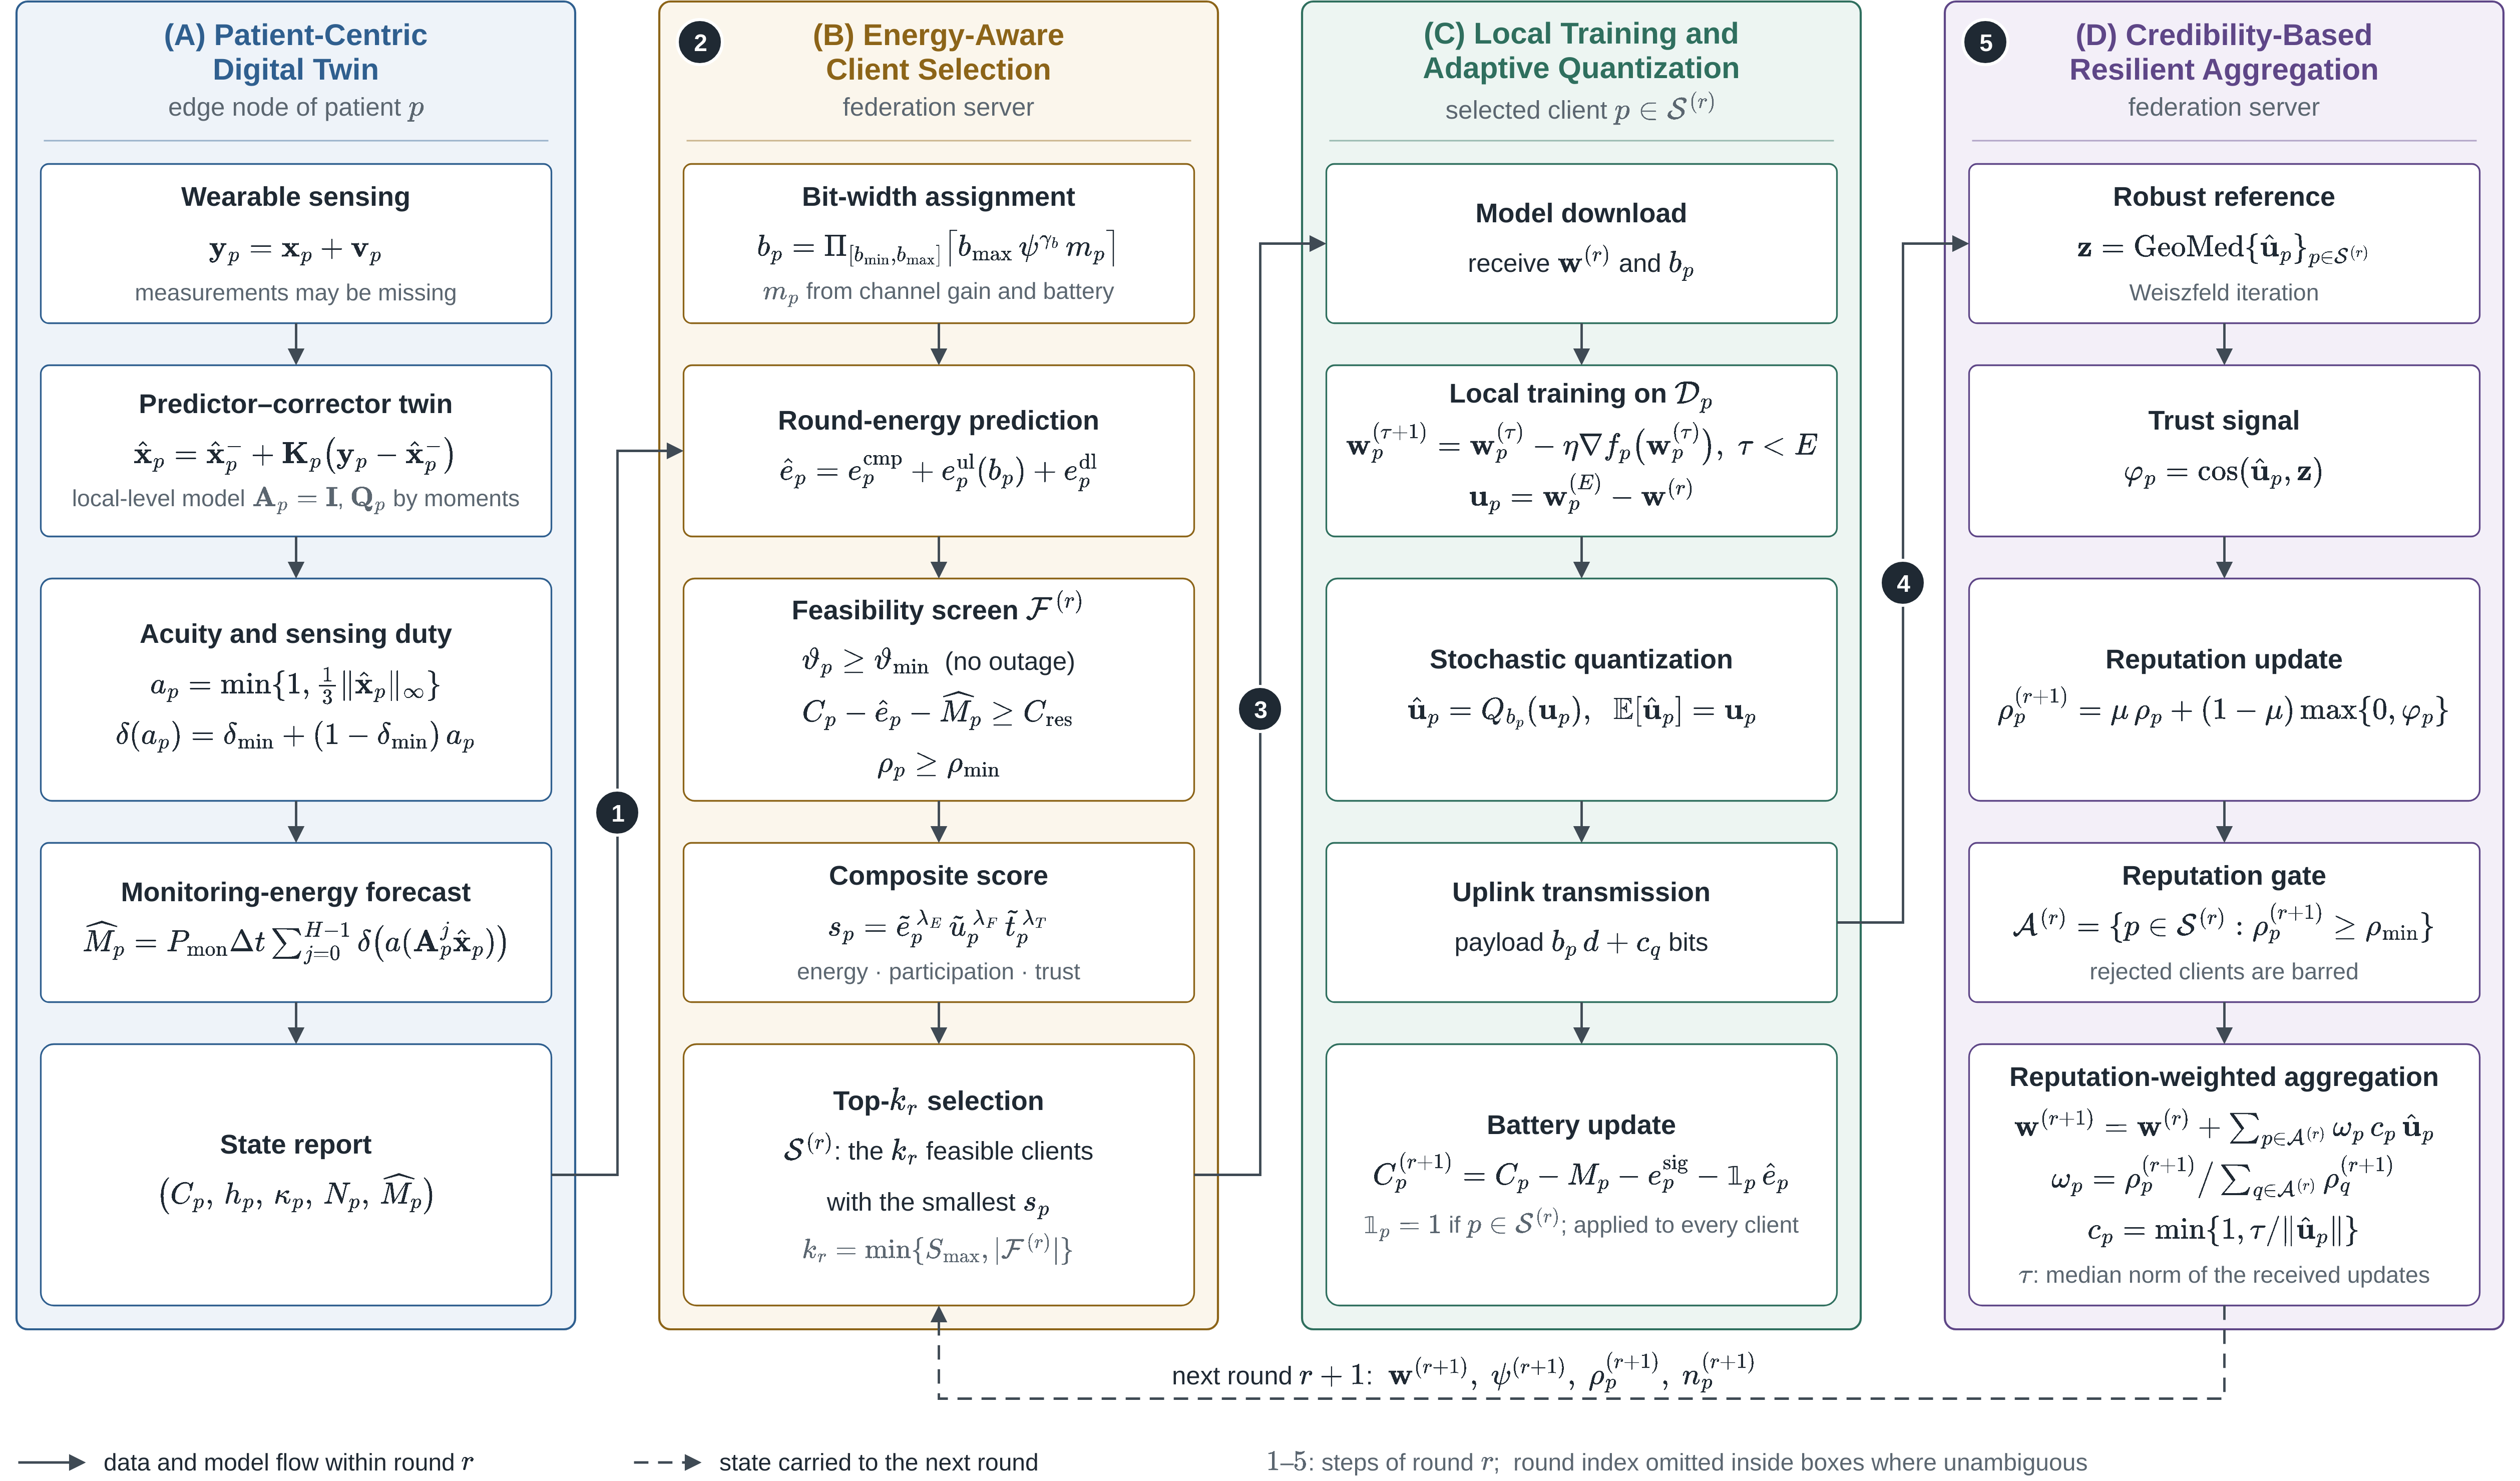
\includegraphics[width=\textwidth]{figures/fig_framework.png}
	\revcap{E6, R1.7(6), R2.6}{Architecture of ATEF-DT: (A)~patient-centric digital twin, (B)~energy-aware client selection, (C)~local training and adaptive quantization, and (D)~credibility-based resilient aggregation. Numbers 1--5 mark the steps of a round; the dashed arrow carries the state to the next round.}
	\label{fig:architecture}
\end{figure*}

\begin{table}[t]
	\centering
	\revcap{R1.7(8)}{Notation.}
	\label{tab:notation}
	\footnotesize
	\setlength{\tabcolsep}{3pt}
	\begin{tabularx}{\columnwidth}{l >{\raggedright\arraybackslash}X}
		\toprule
		\textbf{Symbol} & \textbf{Meaning} \\
		\midrule
		$\cP$, $P$ & set and number of clients \\
		$R$, $S_{\max}$ & number of rounds; per-round selection budget \\
		$\mathcal{D}_p$, $N_p$, $N$ & local data set, its size, total number of samples \\
		$\w^{(r)}\in\mathbb{R}^d$ & global model at round $r$ \\
		$\uu_p^{(r)}$, $\uh_p^{(r)}$ & local update of client $p$; quantized update received by the server \\
		$\eta$, $E$ & learning rate; number of local passes \\
		$\cF^{(r)}$, $\cS^{(r)}$, $\cA^{(r)}$ & feasible, selected and accepted sets \\
		$C_p^{(r)}$, $C_{\mathrm{res}}$ & residual battery energy; reserve \\
		$\kappa_p$, $h_p^{(r)}$, $\vartheta_p^{(r)}$ & computation factor; channel power gain; uplink spectral efficiency \\
		$\hat e_p^{(r)}$ & predicted energy of the round for client $p$ \\
		$\hat{\x}_p^{(r)}$, $a_p^{(r)}$, $\delta(\cdot)$ & twin state estimate; acuity; sensing duty \\
		$M_p^{(r)}$, $\widehat{M}_p^{(r)}$ & monitoring energy of a round; its forecast over $H$ rounds \\
		$b_p^{(r)}$, $\psi^{(r)}$ & bit-width; stability surrogate \\
		$\z^{(r)}$, $\varphi_p^{(r)}$ & geometric-median reference; cosine trust signal \\
		$\rho_p^{(r)}$, $\mu$, $\rho_{\min}$ & reputation; forgetting factor; threshold \\
		$c_p^{(r)}$, $\omega_p^{(r)}$, $\beta_p^{(r)}$ & clipping factor; reputation weight; coefficient $\omega_p c_p$ \\
		$n_p^{(r)}$ & number of rounds before $r$ in which $p$ was selected \\
		$\tilde e_p,\tilde u_p,\tilde t_p$ & energy, participation and trust factors \\
		$\lambda_E,\lambda_F,\lambda_T$ & exponents of the score \\
		\bottomrule
	\end{tabularx}
\end{table}

\subsection{Problem Formulation}
\label{subsec:problem}
The learning objective is the empirical risk over all clients,
\begin{equation}
	F(\w)=\sum_{p\in\cP}\frac{N_p}{N}\,f_p(\w),\qquad f_p(\w)=\frac{1}{N_p}\sum_{(\x,y)\in\mathcal{D}_p}\ell(\w;\x,y),
	\label{eq:objective}
\end{equation}
where $\ell$ is the loss of one sample; this is the standard federated objective, in which each client counts in proportion to its data~\cite{mcmahan2017communication,kairouz2021advances}. The scheduler chooses, in every round, the selected set $\cS^{(r)}$ and the bit-widths $b_p^{(r)}$. Three quantities describe the cost of a schedule over the horizon: the device energy, the disparity of participation and the exposure to updates of low credibility,
\begin{equation}
	\begin{aligned}
		E_{\mathrm{tot}}&=\sum_{r=0}^{R-1}\sum_{p\in\cS^{(r)}}\hat e_p^{(r)}, \qquad D_{\mathrm{part}}=1-J\bigl(\mathbf{n}^{(R)}\bigr),\\
		T_{\mathrm{exp}}&=\sum_{r=0}^{R-1}\sum_{p\in\cS^{(r)}}\bigl(1-\rho_p^{(r)}\bigr),
	\end{aligned}
	\label{eq:criteria}
\end{equation}
where $J(\mathbf{n})=(\sum_p n_p)^2/(P\sum_p n_p^2)$ is the Jain index~\cite{jain1984quantitative} of the participation counts. The index equals one when all clients have taken part equally often and $1/P$ when a single client has taken part every time, so $D_{\mathrm{part}}$ grows as participation concentrates on a few clients. The design problem is the multi-objective program
\begin{equation}
	\begin{aligned}
		\min_{\{\cS^{(r)},\,b^{(r)}\}}\quad & \bigl(F(\w^{(R)}),\;E_{\mathrm{tot}},\;D_{\mathrm{part}},\;T_{\mathrm{exp}}\bigr)\\
		\text{s.t.}\quad & |\cS^{(r)}|\le S_{\max},\quad b_{\min}\le b_p^{(r)}\le b_{\max},\\
		& C_p^{(r)}-\hat e_p^{(r)}-\widehat{M}_p^{(r)}\ge C_{\mathrm{res}}\quad\text{for all } p\in\cS^{(r)} \text{ and all } r .
	\end{aligned}
	\label{eq:designproblem}
\end{equation}
The last constraint protects the clinical function of the device: a client may train only if, after paying for the round, it keeps enough energy to monitor its patient over the next $H$ rounds, with the forecast $\widehat{M}_p^{(r)}$ defined in Section~\ref{subsec:twin}.

\rtag{E2, R1.2, R2.2}\begin{revblock}Problem~\eqref{eq:designproblem} cannot be solved online. The final loss depends on updates that have not yet been computed, the channel gains are revealed one round at a time, and the reputations are produced by the procedure itself. ATEF-DT therefore does not solve~\eqref{eq:designproblem}. It applies a myopic rule in each round, and the rule is a heuristic. What the rule optimizes is the per-round surrogate
\begin{equation}
	\min_{\cS\subseteq\cF^{(r)},\;|\cS|=k_r}\;\sum_{p\in\cS}\bigl(\lambda_E\ln\tilde e_p+\lambda_F\ln\tilde u_p+\lambda_T\ln\tilde t_p\bigr),
	\label{eq:roundproblem}
\end{equation}
with $k_r=\min\{S_{\max},|\cF^{(r)}|\}$, where $\cF^{(r)}$ is the feasible set and $\tilde e_p,\tilde u_p,\tilde t_p>0$ are per-round criteria defined in Section~\ref{subsec:score}. Problem~\eqref{eq:roundproblem} is a weighted-product scalarization~\cite{marler2004survey} of the three per-round criteria. It is not the Lagrangian of~\eqref{eq:designproblem}, and its exponents are preference weights, not multipliers: a Lagrangian relaxation of additive long-run costs leads to an additive per-round index, such as the drift-plus-penalty rule that serves as a baseline in Section~\ref{subsec:schedulers}. No equivalence between~\eqref{eq:roundproblem} and~\eqref{eq:designproblem} is claimed. The product form is a design choice. Its provable consequences are Propositions~\ref{prop:optimal}--\ref{prop:scale}, and its standing against additive and sequential alternatives is an empirical matter that Section~\ref{subsec:schedulers} examines.\end{revblock}

\subsection{Patient-Centric Digital Twin}
\label{subsec:twin}
The twin of patient $p$ keeps a device state and a physiological state. The device state $(C_p^{(r)},\kappa_p,h_p^{(r)},n_p^{(r)},\rho_p^{(r)})$ collects the residual battery energy, the computation factor, the channel gain, the participation count and the reputation; the first three are measured at the edge node and the last two are maintained by the server. Before selection, every reachable edge node sends a state report of five 32-bit fields, $(C_p^{(r)},h_p^{(r)},\kappa_p,N_p,\widehat{M}_p^{(r)})$.

\rtag{R1.7(2)}\begin{revblock}The physiological state $\x_p^{(r)}\in\mathbb{R}^m$ holds $m$ vital-sign deviations in standardized units (zero mean and unit variance at rest). It follows a linear-Gaussian state-space model in which every variable is observed directly,
\begin{equation}
	\x_p^{(r+1)}=\mathbf{A}_p\x_p^{(r)}+\boldsymbol{\omega}_p^{(r)},\qquad \y_p^{(r)}=\x_p^{(r)}+\mathbf{v}_p^{(r)},
	\label{eq:twinmodel}
\end{equation}
with $\boldsymbol{\omega}_p^{(r)}\sim\mathcal{N}(\mathbf{0},\mathbf{Q}_p)$ and $\mathbf{v}_p^{(r)}\sim\mathcal{N}(\mathbf{0},\mathbf{R}_p)$. The twin is the Kalman predictor--corrector~\cite{kalman1960new} of this model. With estimate $\hat{\x}_p$ and error covariance $\boldsymbol{\Sigma}_p$,
\begin{align}
	\hat{\x}_p^{-}&=\mathbf{A}_p\hat{\x}_p^{(r-1)}, & \boldsymbol{\Sigma}_p^{-}&=\mathbf{A}_p\boldsymbol{\Sigma}_p^{(r-1)}\mathbf{A}_p^{\top}+\mathbf{Q}_p, \label{eq:predict}\\
	\mathbf{K}_p&=\boldsymbol{\Sigma}_p^{-}\bigl(\boldsymbol{\Sigma}_p^{-}+\mathbf{R}_p\bigr)^{-1}, & \hat{\x}_p^{(r)}&=\hat{\x}_p^{-}+\mathbf{K}_p\bigl(\y_p^{(r)}-\hat{\x}_p^{-}\bigr), \label{eq:correct}
\end{align}
and $\boldsymbol{\Sigma}_p^{(r)}=(\mathbf{I}-\mathbf{K}_p)\boldsymbol{\Sigma}_p^{-}$. In words, the twin first predicts the state from its previous estimate and then corrects the prediction by a fraction of the new measurement; the gain $\mathbf{K}_p$ makes that fraction large when the sensor is accurate relative to the model and small when it is noisy. When no measurement arrives in a round, the correction is skipped, $\hat{\x}_p^{(r)}=\hat{\x}_p^{-}$ and $\boldsymbol{\Sigma}_p^{(r)}=\boldsymbol{\Sigma}_p^{-}$, and a staleness counter is incremented; the counter is reset by the next measurement.

None of the matrices is a free parameter. The transition matrix is that of the local-level model, $\mathbf{A}_p=\mathbf{I}$, which does not assume that a patient returns to a resting state. The process noise is estimated by the method of moments from a monitoring window of $T_w$ samples recorded before training: the first differences of the window have variance $\mathbf{Q}_p+2\mathbf{R}_p$, so $\mathbf{Q}_p=\operatorname{diag}\bigl(\max\{\widehat{\operatorname{Var}}(\Delta\y_p)-2\sigma_v^2,\,10^{-3}\}\bigr)$. The measurement covariance $\mathbf{R}_p=\sigma_v^2\mathbf{I}$ is the sensor specification. The gain $\mathbf{K}_p$ is not estimated; it is computed in every round from~\eqref{eq:correct}. The filter is initialized with the last sample of the window and $\boldsymbol{\Sigma}_p=\mathbf{R}_p$. A first-order autoregressive alternative, in which $\mathbf{A}_p$ is fitted to the window by ridge least squares, is implemented as well and is compared with the local-level model in Table~\ref{tab:twin}. Table~\ref{tab:twincfg} lists the configuration.\end{revblock}

The acuity is the largest standardized deviation, saturated at three standard deviations, and the sensing duty grows linearly with it,
\begin{equation}
	a_p^{(r)}=\min\bigl\{1,\;\tfrac{1}{3}\norm{\hat{\x}_p^{(r)}}_{\infty}\bigr\},\qquad \delta(a)=\delta_{\min}+(1-\delta_{\min})\,a .
	\label{eq:acuity}
\end{equation}
Monitoring consumes $M_p^{(r)}=P_{\mathrm{mon}}\,\Delta t\,\delta(a_p^{(r)})$ in a round of duration $\Delta t$. The twin forecasts the monitoring energy of the next $H$ rounds from its own prediction,
\begin{equation}
	\widehat{M}_p^{(r)}=P_{\mathrm{mon}}\,\Delta t\sum_{j=0}^{H-1}\delta\Bigl(a\bigl(\mathbf{A}_p^{\,j}\hat{\x}_p^{(r)}\bigr)\Bigr),
	\label{eq:forecast}
\end{equation}
and, when the staleness counter exceeds $\tau_{\max}$, it reports the conservative value $H\,P_{\mathrm{mon}}\Delta t$.

A client is battery-feasible in round $r$ when training would leave the reserve intact after the forecast monitoring drain,
\begin{equation}
	C_p^{(r)}-\hat e_p^{(r)}-\widehat{M}_p^{(r)}\;\ge\;C_{\mathrm{res}} .
	\label{eq:screen}
\end{equation}
The screen asks whether the device can pay for this round of training and still keep enough energy to monitor the patient for the next $H$ rounds. This is the point at which the physiological twin acts on the scheduler: a patient whose condition is deteriorating is monitored more intensively, the forecast drain rises, and the device is withdrawn from training earlier than an instantaneous battery test would withdraw it.

\begin{table}[t]
	\centering
	\revcap{R1.7(2), E5}{Digital-twin configuration.}
	\label{tab:twincfg}
	\footnotesize
	\begin{tabularx}{\columnwidth}{>{\raggedright\arraybackslash}X l}
		\toprule
		\textbf{Quantity} & \textbf{Value} \\
		\midrule
		State dimension $m$ & 3 \\
		Transition model $\mathbf{A}_p$ & $\mathbf{I}$ (local level) \\
		Identification window $T_w$ & 30 samples \\
		Process noise $\mathbf{Q}_p$ & method of moments on the window \\
		Measurement noise $\mathbf{R}_p$ & $\sigma_v^2\mathbf{I}$ (sensor specification) \\
		Ridge parameter (autoregressive alternative) & $10^{-2}$ \\
		Forecast horizon $H$ & 5 rounds \\
		Staleness bound $\tau_{\max}$ & 3 rounds \\
		Minimum sensing duty $\delta_{\min}$ & 0.2 \\
		Monitoring power $P_{\mathrm{mon}}$; round duration $\Delta t$ & 2 mW; 60 s \\
		\bottomrule
	\end{tabularx}
\end{table}

\subsection{Energy Model}
\label{subsec:energy}
The energy of a round has a computation part, an uplink part and a downlink part, following the modelling of~\cite{tran2019federated,yang2021energy}. Local training costs
\begin{equation}
	e_p^{\mathrm{cmp}}=\alpha\,\kappa_p\,N_p\,d\,E ,
	\label{eq:ecmp}
\end{equation}
so that the computation energy grows linearly with the amount of data, the model size and the number of local passes. Here $\alpha$ is the energy of one multiply--accumulate operation on a reference device, $\kappa_p$ is the device factor, and $N_p d$ is the number of such operations in one pass through a model with $d$ parameters. The channel is Rayleigh block fading: the power gain $h_p^{(r)}=\bar h_p\,g_p^{(r)}$ is the product of a mean gain $\bar h_p$ and a unit-mean exponential variable $g_p^{(r)}$ that is constant within a round. The uplink spectral efficiency is
\begin{equation}
	\vartheta_p^{(r)}=\log_2\!\Bigl(1+\frac{P_{\mathrm{tx}}\,h_p^{(r)}}{\sigma^2W\Gamma}\Bigr)\quad\text{bit/s/Hz},
	\label{eq:rate}
\end{equation}
with transmit power $P_{\mathrm{tx}}$, bandwidth $W$, noise power spectral density $\sigma^2$ and signal-to-noise gap $\Gamma$; this is the Shannon rate used in wireless FL models~\cite{yang2021energy}, and a weaker channel gives a lower rate and therefore a longer, costlier transmission. A payload of $B_p^{(r)}$ bits (Section~\ref{subsec:quant}) occupies the channel for $(1+\nu)B_p^{(r)}/(W\vartheta_p^{(r)})$ seconds, where $\nu$ is the protocol overhead, and the energy drawn from the battery is~\cite{yang2021energy}
\begin{equation}
	e_p^{\mathrm{ul}}=\frac{P_{\mathrm{tx}}}{\eta_{\mathrm{PA}}\,(1-\varepsilon_{\mathrm{PER}})}\cdot\frac{(1+\nu)\,B_p^{(r)}}{W\,\vartheta_p^{(r)}},
	\label{eq:eul}
\end{equation}
where $\eta_{\mathrm{PA}}$ is the efficiency of the power amplifier and $\varepsilon_{\mathrm{PER}}$ the packet error rate, which inflates the airtime by retransmissions. \rtag{R1.5}\rev{The broadcast of the global model is not free for the device: receiving $32d$ bits at the downlink rate keeps the receive chain active and costs
\begin{equation}
	e_p^{\mathrm{dl}}=P_{\mathrm{rx}}\cdot\frac{(1+\nu)\,32\,d}{W\log_2\!\bigl(1+P_{\mathrm{BS}}\,h_p^{(r)}/(\sigma^2W\Gamma)\bigr)},
	\label{eq:edl}
\end{equation}
with receive power $P_{\mathrm{rx}}$ and base-station transmit power $P_{\mathrm{BS}}$, by the same rate model~\cite{tran2019federated}.} The predicted energy of a round is $\hat e_p^{(r)}=e_p^{\mathrm{cmp}}+e_p^{\mathrm{ul}}+e_p^{\mathrm{dl}}$. A device is in outage, and is not scheduled, when $\vartheta_p^{(r)}<\vartheta_{\min}$. The battery evolves as
\begin{equation}
	C_p^{(r+1)}=\max\Bigl\{0,\;C_p^{(r)}-\mathbb{1}[p\in\cS^{(r)}]\,\hat e_p^{(r)}-M_p^{(r)}-e_p^{\mathrm{sig}}\Bigr\},
	\label{eq:battery}
\end{equation}
where $e_p^{\mathrm{sig}}$ is the uplink energy~\eqref{eq:eul} of the 160-bit state report. Every device pays for monitoring and reporting in every round, and only the selected devices also pay for training and communication. Only device-side energy is counted; the energy radiated by the base station is not.

\subsection{Energy-Aware Client Selection}
\label{subsec:score}
The feasible set $\cF^{(r)}$ contains the clients that are not in outage, have a non-empty battery, pass the screen~\eqref{eq:screen} and have a reputation $\rho_p^{(r)}\ge\rho_{\min}$, where the reputation is maintained by the credibility engine of Section~\ref{subsec:credibility}. Three factors are computed over $\cF^{(r)}$, each oriented so that a smaller value is preferable:
\begin{align}
	\tilde e_p&=\frac{\hat e_p^{(r)}-\min_{q}\hat e_q^{(r)}}{\max_{q}\hat e_q^{(r)}-\min_{q}\hat e_q^{(r)}+\varepsilon_0}+\varepsilon_0, \label{eq:efactor}\\
	\tilde u_p&=\frac{n_p^{(r)}+1}{\max_{q}n_q^{(r)}+1}, \label{eq:ufactor}\\
	\tilde t_p&=\bigl(1-\rho_p^{(r)}\bigr)+\varepsilon_0, \label{eq:tfactor}
\end{align}
where the minima and maxima run over $q\in\cF^{(r)}$ and $\varepsilon_0>0$ keeps the factors positive. The score is the weighted product
\begin{equation}
	s_p^{(r)}=\tilde e_p^{\,\lambda_E}\;\tilde u_p^{\,\lambda_F}\;\tilde t_p^{\,\lambda_T},
	\label{eq:score}
\end{equation}
and $\cS^{(r)}$ consists of the $k_r$ feasible clients with the smallest scores, ties being broken by client index. A client therefore ranks well when it is cheap to train, has been selected rarely and has a high reputation; the exponents set how strongly each of these counts. Because the factors are multiplied, each criterion acts through relative changes: halving a client's energy factor lowers its score by the factor $2^{-\lambda_E}$, whatever the values of the other two factors. This is why the ranking needs no normalization of the criteria against each other (Proposition~\ref{prop:scale}), a known property of product scalarization~\cite{marler2004survey}. The following properties are proved in \ref{app:score}.

\begin{proposition}[Per-round optimality and non-dominance]
	\label{prop:optimal}
	(a)~The set $\cS^{(r)}$ is an optimal solution of the per-round problem~\eqref{eq:roundproblem}. (b)~If $\lambda_E,\lambda_F,\lambda_T>0$, no client in $\cF^{(r)}\setminus\cS^{(r)}$ dominates a client in $\cS^{(r)}$, where $q$ dominates $p$ if $(\tilde e_q,\tilde u_q,\tilde t_q)\le(\tilde e_p,\tilde u_p,\tilde t_p)$ componentwise with at least one strict inequality.
\end{proposition}

\begin{proposition}[Sequential pipelines]
	\label{prop:pipeline}
	Let $\lambda_E,\lambda_F>0$ and $k_r<\bar k<|\cF^{(r)}|$. Consider a pipeline that first keeps the $\bar k$ feasible clients with the smallest value of one of the factors $\tilde e_p$ and $\tilde u_p$, and then selects among them the $k_r$ clients with the smallest value of the other. For either order of the two factors and for every $\theta>1$, there is an instance on which the product of the scores~\eqref{eq:score} of the clients selected by the pipeline exceeds the minimum of that product over all subsets of $k_r$ feasible clients by a factor larger than $\theta$.
\end{proposition}

\begin{proposition}[Invariance to rescaling]
	\label{prop:scale}
	Let $c_E,c_F,c_T>0$. Replacing $(\tilde e_p,\tilde u_p,\tilde t_p)$ by $(c_E\tilde e_p,c_F\tilde u_p,c_T\tilde t_p)$ for all $p$ leaves the ranking by~\eqref{eq:score}, and hence $\cS^{(r)}$, unchanged. The ranking by a weighted sum $\lambda_E\tilde e_p+\lambda_F\tilde u_p+\lambda_T\tilde t_p$ is not invariant under the same transformation.
\end{proposition}

\rtag{E2, R1.2, R2.2}\begin{revblock}\begin{remark}[Scope of the propositions]
	Proposition~\ref{prop:optimal} concerns the per-round surrogate and says nothing about the long-run problem~\eqref{eq:designproblem}. Proposition~\ref{prop:pipeline} is a worst-case statement about a class of pipelines; how such pipelines behave on typical instances is measured in Section~\ref{subsec:schedulers}. Proposition~\ref{prop:scale} covers multiplicative rescaling, such as a change of units; the ranking is not invariant to a shift of a factor, and it does depend on the exponents, which remain to be chosen. The practical content of Proposition~\ref{prop:scale} is that the criteria need not be normalized against each other, whereas the operating point of a weighted sum moves with the scale of each term.
\end{remark}\end{revblock}

\subsection{Local Training and Adaptive Quantization}
\label{subsec:quant}\label{subsec:local}
A selected client starts from the global model, $\w_p^{(r,0)}=\w^{(r)}$, performs $E$ full-batch gradient steps on its own data,
\begin{equation}
	\w_p^{(r,\tau+1)}=\w_p^{(r,\tau)}-\eta\,\nabla f_p\bigl(\w_p^{(r,\tau)}\bigr),\qquad \tau=0,\dots,E-1,
	\label{eq:local}
\end{equation}
and forms the update $\uu_p^{(r)}=\w_p^{(r,E)}-\w^{(r)}$. The reference methods aggregate with data-volume weights as in FedAvg~\cite{mcmahan2017communication},
\begin{equation}
	\w^{(r+1)}=\w^{(r)}+\sum_{p\in\cS^{(r)}}\frac{N_p}{\sum_{q\in\cS^{(r)}}N_q}\,\uu_p^{(r)} .
	\label{eq:fedavg}
\end{equation}
ATEF-DT replaces~\eqref{eq:fedavg} by the rule of Section~\ref{subsec:credibility}.

After training, a client that is assigned $b$ bits by the server maps its update $\uu\in\mathbb{R}^d$ to a grid of $2^b$ levels between $u_{\min}=\min_i u_i$ and $u_{\max}=\max_i u_i$ with step $\Delta=(u_{\max}-u_{\min})/(2^b-1)$, and rounds every coordinate stochastically,
\begin{equation}
	Q_b(\uu)_i=u_{\min}+\Delta\Bigl(\Bigl\lfloor\frac{u_i-u_{\min}}{\Delta}\Bigr\rfloor+\xi_i\Bigr),
	\label{eq:quant}
\end{equation}
where $\xi_i$ is a Bernoulli variable whose mean is the fractional part of $(u_i-u_{\min})/\Delta$. The quantizer is unbiased, $\E[Q_b(\uu)]=\uu$, and the error of a coordinate is smaller than $\Delta$ in magnitude~\cite{alistarh2017qsgd}. The payload is $B=b\,d+c_q$ bits, where $c_q=64$ bits carry $u_{\min}$ and $u_{\max}$. The server receives $\uh_p^{(r)}=Q_{b_p^{(r)}}(\uu_p^{(r)})$.

\rtag{R1.7(1)}\begin{revblock}The server tracks the size of its own steps,
\begin{equation}
	\psi^{(0)}=1,\qquad \psi^{(r)}=\frac{\norm{\w^{(r)}-\w^{(r-1)}}}{\norm{\w^{(1)}-\w^{(0)}}}\quad\text{for } r\ge 1 .
	\label{eq:psi}
\end{equation}
The surrogate is evaluated at the start of round $r$, before the bit-widths are assigned. No update exists before the first aggregation, so $\psi^{(0)}=1$ by definition, and $\psi^{(1)}=1$ follows from~\eqref{eq:psi}; the first two rounds therefore use the largest bit-width, and the rule becomes adaptive from round $r=2$. The surrogate uses server-side quantities only and requires no gradient norm from the clients.\end{revblock}

The bit-width of client $p$ decreases as training stabilizes and is reduced further for clients with a weak channel or a low battery,
\begin{equation}
	b_p^{(r)}=\Bigl\lceil\min\bigl\{b_{\max},\,\max\{b_{\min},\;b_{\max}\,(\min\{\psi^{(r)},1\})^{\gamma_b}\,m_p^{(r)}\}\bigr\}\Bigr\rceil,
	\label{eq:bitwidth}
\end{equation}
\begin{equation}
	m_p^{(r)}=\min\Bigl\{1,\sqrt{h_p^{(r)}/h_{\mathrm{ref}}}\Bigr\}\cdot\min\bigl\{1,\;C_p^{(r)}/C_{\mathrm{ref}}\bigr\},
	\label{eq:mod}
\end{equation}
where $h_{\mathrm{ref}}$ is the mean of the clients' mean gains and $C_{\mathrm{ref}}$ a battery level below which the payload is coarsened. The rule thus spends many bits early in training, when updates are large and informative, and few bits later; within a round, clients with a weak channel or a low battery send coarser updates, since each bit costs them more energy.

The uplink traffic of a run is $\sum_{r}\sum_{p\in\cS^{(r)}}(b_p^{(r)}d+c_q)$ bits. With $\bar b$ the mean bit-width over all transmissions, the reduction relative to 32-bit transmission of the same updates is
\begin{equation}
	\chi=\frac{32}{\bar b+c_q/d} .
	\label{eq:compression}
\end{equation}
\rtag{R1.5}\rev{Quantization acts on the uplink only. The global model is broadcast at full precision, $32d$ bits per selected client and round, and Section~\ref{subsec:energyres} reports the uplink, the downlink and the state reports separately.}

\subsection{Credibility-Based Resilient Aggregation}
\label{subsec:credibility}
\rtag{R1.4}\rev{Every quantity in this subsection is computed from the vectors $\uh_p^{(r)}$ that the server receives, that is, from the quantized updates; the server never has access to $\uu_p^{(r)}$.}

The reference direction is the geometric median of the received updates,
\begin{equation}
	\z^{(r)}=\arg\min_{\z\in\mathbb{R}^d}\sum_{p\in\cS^{(r)}}\norm{\uh_p^{(r)}-\z},
	\label{eq:gm}
\end{equation}
computed by the Weiszfeld iteration~\cite{pillutla2022robust}. The geometric median is robust because it cannot be moved arbitrarily far by fewer than half of the points. The trust signal of a client is its cosine to the reference, in the spirit of FLTrust~\cite{cao2021fltrust}, which scores updates by their direction rather than their size,
\begin{equation}
	\varphi_p^{(r)}=\frac{\langle\uh_p^{(r)},\z^{(r)}\rangle}{\norm{\uh_p^{(r)}}\,\norm{\z^{(r)}}}\in[-1,1].
	\label{eq:cos}
\end{equation}

The reputation of a selected client is updated by exponential forgetting of the rectified signal,
\begin{equation}
	\rho_p^{(r+1)}=\mu\,\rho_p^{(r)}+(1-\mu)\max\{0,\varphi_p^{(r)}\},\qquad p\in\cS^{(r)},
	\label{eq:rep}
\end{equation}
with $\rho_p^{(0)}=1$; the reputation of a client that is not selected does not change. A client that keeps pointing in the same direction as the reference keeps a high reputation, while one that repeatedly points away loses a fraction $1-\mu$ of its reputation at each submission.

\begin{lemma}[Range and exclusion time]
	\label{lem:rep}
	(a)~$\rho_p^{(r)}\in[0,1]$ for all $p$ and $r$. (b)~If the trust signal of a client is non-positive in each of its submissions from a point at which its reputation is $\rho_0>\rho_{\min}$, the reputation first falls below $\rho_{\min}$ at submission number
	\begin{equation}
		k^{\star}=\Bigl\lfloor\frac{\ln(\rho_{\min}/\rho_0)}{\ln\mu}\Bigr\rfloor+1 .
		\label{eq:kstar}
	\end{equation}
\end{lemma}
\begin{proof}
	(a)~The update~\eqref{eq:rep} is a convex combination of $\rho_p^{(r)}\in[0,1]$ and $\max\{0,\varphi_p^{(r)}\}\in[0,1]$. (b)~With a non-positive signal, $\rho$ is multiplied by $\mu$ at each submission, so after $k$ submissions it equals $\mu^k\rho_0$, which is below $\rho_{\min}$ exactly when $k>\ln(\rho_{\min}/\rho_0)/\ln\mu$.
\end{proof}
With $\mu=0.6$, $\rho_{\min}=0.05$ and $\rho_0=1$, the bound is $k^{\star}=\V{kstar}$. The bound counts submissions, not rounds, and it presupposes a signal that is never positive; Section~\ref{subsec:byzantine} shows that this premise often fails in practice.

A client whose reputation is below $\rho_{\min}$ at the start of a round is not admitted to the feasible set. Because the reputation changes only when a client is selected, exclusion is permanent. After the update~\eqref{eq:rep}, the accepted set is
\begin{equation}
	\cA^{(r)}=\bigl\{p\in\cS^{(r)}:\rho_p^{(r+1)}\ge\rho_{\min}\bigr\}.
	\label{eq:accept}
\end{equation}

Received updates are clipped to the median norm, a standard defence against updates of inflated size~\cite{karimireddy2021learning}, $\tau^{(r)}=\operatorname{median}_{p\in\cS^{(r)}}\norm{\uh_p^{(r)}}$ and $c_p^{(r)}=\min\{1,\tau^{(r)}/\norm{\uh_p^{(r)}}\}$, and the accepted updates are averaged with reputation weights,
\begin{equation}
	\w^{(r+1)}=\w^{(r)}+\sum_{p\in\cA^{(r)}}\omega_p^{(r)}\,c_p^{(r)}\,\uh_p^{(r)},\qquad \omega_p^{(r)}=\frac{\rho_p^{(r+1)}}{\sum_{q\in\cA^{(r)}}\rho_q^{(r+1)}} .
	\label{eq:agg}
\end{equation}

\rtag{R1.4}\begin{revblock}Rule~\eqref{eq:agg} is the only aggregation rule of ATEF-DT. The weights $\omega_p^{(r)}$ are non-negative and sum to one over the accepted set. They contain no data-volume factor: the sizes $N_p$ are reported by the clients themselves, and a weight proportional to a self-reported quantity can be inflated by an adversary. The price is a bias when the data volumes are unequal, which Section~\ref{subsec:bias} bounds and Section~\ref{subsec:fairres} measures. The coefficients actually applied are $\beta_p^{(r)}=\omega_p^{(r)}c_p^{(r)}$, and their sum
\begin{equation}
	s^{(r)}=\sum_{p\in\cA^{(r)}}\beta_p^{(r)}\in(0,1]
	\label{eq:stepscale}
\end{equation}
is smaller than one whenever an accepted update is clipped. At least half of the received updates have a norm not larger than the median, so when no update is rejected, $s^{(r)}\ge\rho_{\min}/2$. The quantity $s^{(r)}$ acts as a step-size scale in the convergence analysis.\end{revblock}

\subsection{Threat Model and Scope of the Privacy Protection}
\label{subsec:privacy}
The server is honest and the links are authenticated. A subset of the clients is Byzantine: such a client knows the protocol, may collude with other Byzantine clients and may submit any vector. The trust signal and the aggregation rule are computed within a round from at most $S_{\max}$ received updates, so the engine can rely only on an honest majority within each selected set. Its domain is therefore limited as follows.

\begin{assumption}[Domain of the credibility engine]
	\label{ass:threat}
	In every round, the Byzantine clients are fewer than half of the selected set, and their updates are not concentrated closely enough to move the geometric median away from the honest updates.
\end{assumption}

When Assumption~\ref{ass:threat} is violated, the reference~\eqref{eq:gm} can be captured: the cosine then rewards the adversaries and penalizes the honest clients. The fraction of rounds in which the first part of the assumption fails is measured in Section~\ref{subsec:byzantine}, and the second part is tested with a colluding adversary.

\rtag{R1.6}\begin{revblock}The privacy adversary is an honest-but-curious server, or an eavesdropper on the uplink, that follows the protocol and observes three things: the quantized updates $\uh_p^{(r)}$, the state reports, and the participation pattern, that is, which clients are selected in which rounds. Patient records never leave the device, but this data locality is not a formal privacy guarantee, and three channels remain open. First, updates can be inverted to recover training samples~\cite{zhu2019deep} and support membership inference; stochastic quantization~\eqref{eq:quant} adds bounded noise for compression and provides no differential-privacy guarantee. Second, the participation pattern reveals the resources of a device, because the score depends on its energy cost. Third, and specific to this design, the forecast $\widehat{M}_p^{(r)}$ in the state report is a function of the patient's acuity, so that the report, and indirectly the withdrawal of a device from training, discloses information about the patient's condition.

ATEF-DT provides no formal protection against these channels. Two standard mechanisms could be added, each at a cost. Client-level DP~\cite{wei2020federated} requires a fixed clipping bound in place of the data-dependent median bound and adds noise that lowers the cosine~\eqref{eq:cos} of honest clients; moreover, the amplification of privacy by random participation, which the analyses in~\cite{li2025differentially,li2025federated} exploit, does not apply to a selection rule that is deterministic given the state. Secure aggregation~\cite{bonawitz2017practical} hides individual updates from the server and is therefore incompatible with a credibility engine that inspects each update. Reconciling the three goals, and coarsening or encrypting the state report, are left to future work; the framework as evaluated here should be read as offering data locality and integrity checks, not formal privacy.\end{revblock}

\subsection{Algorithm and Complexity}
\label{subsec:algorithm}
Algorithm~\ref{alg:atef} summarizes a run. The order of the steps matters in two places: the surrogate $\psi^{(r)}$ and the bit-widths are computed before selection, from quantities that are available at the start of the round, and the reputations are updated before the gate and the weights are applied.

\begin{algorithm}[t]
	\caption{ATEF-DT.}
	\label{alg:atef}
	\footnotesize
	\begin{algorithmic}[1]
		\REQUIRE $\w^{(0)}$; $\rho_p^{(0)}=1$, $n_p^{(0)}=0$ for all $p$; parameters of Table~\ref{tab:setup}
		\FOR{$r=0,1,\dots,R-1$}
		\STATE \textbf{Twin layer:} every edge node runs \eqref{eq:predict}--\eqref{eq:correct}, computes $a_p^{(r)}$ and $\widehat{M}_p^{(r)}$ by \eqref{eq:acuity}--\eqref{eq:forecast}, and sends its state report
		\STATE \textbf{Server:} compute $\psi^{(r)}$ by~\eqref{eq:psi} and $b_p^{(r)}$ by~\eqref{eq:bitwidth}; predict $\hat e_p^{(r)}$
		\STATE Form $\cF^{(r)}$: no outage, $C_p^{(r)}>0$, screen~\eqref{eq:screen}, $\rho_p^{(r)}\ge\rho_{\min}$
		\STATE Compute the factors \eqref{eq:efactor}--\eqref{eq:tfactor} and the scores~\eqref{eq:score}; let $\cS^{(r)}$ be the $k_r$ clients with the smallest scores
		\STATE Send $\w^{(r)}$ and $b_p^{(r)}$ to every $p\in\cS^{(r)}$; set $n_p^{(r+1)}=n_p^{(r)}+1$ (the counts of the other clients are unchanged)
		\FOR{each $p\in\cS^{(r)}$ in parallel}
		\STATE Train by~\eqref{eq:local}; form $\uu_p^{(r)}$; upload $\uh_p^{(r)}=Q_{b_p^{(r)}}(\uu_p^{(r)})$
		\ENDFOR
		\STATE Compute the reference $\z^{(r)}$ by~\eqref{eq:gm} and the signals $\varphi_p^{(r)}$ by~\eqref{eq:cos}
		\STATE Update the reputations by~\eqref{eq:rep}; form $\cA^{(r)}$ by~\eqref{eq:accept}
		\STATE Clip and aggregate by~\eqref{eq:agg} to obtain $\w^{(r+1)}$
		\STATE Update the batteries by~\eqref{eq:battery}
		\ENDFOR
		\RETURN $\w^{(R)}$
	\end{algorithmic}
\end{algorithm}

Scoring and selection cost $O(P\log P)$ operations per round. With $k=|\cS^{(r)}|$ received updates, the geometric median costs $O(I\,k\,d)$ for $I$ Weiszfeld iterations, and the cosines, the clipping and the weighted sum cost $O(k\,d)$ each. The server-side overhead of a round is therefore $O(P\log P+I\,k\,d)$; measured times are reported in Section~\ref{subsec:scalability}. On the client, the method adds the quantizer, which is linear in $d$, and the state report.

\section{Convergence Analysis}
\label{sec:convergence}
\rtag{E3, R1.3, R2.3}\begin{revblock}The analysis concerns the update that Algorithm~\ref{alg:atef} actually applies. Selection probabilities and aggregation weights are kept apart: selection decides who transmits, the coefficients $\beta_p^{(r)}$ decide how much each received update counts, and the bias of the procedure depends on their combination. No assumption is made that relates selection probabilities to data proportions. The argument follows the analysis of gradient methods with biased search directions~\cite{ajalloeian2020convergence}; analyses of FedAvg under partial participation~\cite{wang2020tackling} rely on unbiased sampling or on weights proportional to the data volumes, neither of which holds for the rule studied here.

Write $\hat{\g}_p^{(r)}=-\uh_p^{(r)}/\eta$ for the pseudo-gradient that the server receives from client $p$. By~\eqref{eq:agg}, the model evolves as
\begin{equation}
	\w^{(r+1)}=\w^{(r)}-\eta\,\g^{(r)},\qquad \g^{(r)}=\sum_{p\in\cA^{(r)}}\beta_p^{(r)}\,\hat{\g}_p^{(r)} .
	\label{eq:applied}
\end{equation}
Let $\E_r[\cdot]$ denote the expectation conditional on the history up to the start of round $r$; it is taken over the fading, the rounding of the quantizer and any randomness of the clients. Define the expected step scale and the bias of the applied direction,
\begin{equation}
	\bar s_r=\E_r\bigl[s^{(r)}\bigr],\qquad \bb_r=\E_r\bigl[\g^{(r)}\bigr]-\bar s_r\,\nabla F(\w^{(r)}),
	\label{eq:biasdef}
\end{equation}
with $s^{(r)}$ from~\eqref{eq:stepscale}.

\begin{assumption}[Smoothness]
	\label{ass:smooth}
	$F$ is bounded below by $F^{\star}$ and has an $L$-Lipschitz gradient.
\end{assumption}

\begin{assumption}[Bias and variance of the applied update]
	\label{ass:update}
	There are constants $s_{\min}\in(0,1]$, $B\ge 0$ and $V\ge 0$ such that, for every round, $\bar s_r\ge s_{\min}$, $\norm{\bb_r}\le B$ and $\E_r\norm{\g^{(r)}-\E_r[\g^{(r)}]}^2\le V$.
\end{assumption}

\begin{theorem}[Convergence to a neighbourhood]
	\label{thm:convergence}
	Under Assumptions~\ref{ass:smooth} and~\ref{ass:update}, with a learning rate $\eta\le 1/L$,
	\begin{equation}
		\frac{1}{R}\sum_{r=0}^{R-1}\E\norm{\nabla F(\w^{(r)})}^2\;\le\;\frac{2\bigl(F(\w^{(0)})-F^{\star}\bigr)}{\eta\,s_{\min}\,R}+\frac{B^2}{s_{\min}^2}+\frac{L\,\eta\,V}{s_{\min}} .
		\label{eq:bound}
	\end{equation}
\end{theorem}

The proof is given in \ref{app:proofs}. With the learning rate $\eta=\min\{1/L,\,R^{-1/2}\}$, the first and third terms decay as $O(R^{-1/2})$, and the bound tends to $B^2/s_{\min}^2$. The procedure therefore reaches a neighbourhood of a stationary point whose radius is set by the bias; it is not claimed to reach a stationary point of $F$.

\begin{remark}[What the theorem covers]
	\label{rem:scope}
	The selection rule, the gate, the clipping, the reputation weights and the quantizer enter~\eqref{eq:bound} only through $s_{\min}$, $B$ and $V$. The theorem therefore holds for the actual selection rule of Algorithm~\ref{alg:atef}, and equally for any other rule, but it is conditional: the constants are assumed, not derived from the rule. For the step scale, $s^{(r)}\ge\rho_{\min}/2$ whenever no update is rejected (Section~\ref{subsec:credibility}), and the measured values are reported in Section~\ref{subsec:fairres}. The bias has a participation part, which is bounded next, and a part caused by the dependence between the coefficients and the received vectors. Under attack the second part contains the contribution of the adversaries, and no bound on it is claimed outside Assumption~\ref{ass:threat}.
\end{remark}

\subsection{Participation and Weighting Bias}
\label{subsec:bias}
Define the effective aggregation weight of client $p$ in round $r$ and its normalized form,
\begin{equation}
	\pi_p^{(r)}=\E_r\bigl[\beta_p^{(r)}\,\mathbb{1}[p\in\cA^{(r)}]\bigr],\qquad \hat\pi_p^{(r)}=\frac{\pi_p^{(r)}}{\bar s_r},
	\label{eq:effweight}
\end{equation}
so that $\sum_p\pi_p^{(r)}=\bar s_r$ and $\sum_p\hat\pi_p^{(r)}=1$. The effective weight is the product of two things that the earlier formulation conflated: the probability that the client's update is accepted, and the coefficient it then receives. Adding and subtracting $\sum_p\pi_p^{(r)}\nabla f_p(\w^{(r)})$ in~\eqref{eq:biasdef} splits the bias as $\bb_r=\mathbf{c}_{\mathrm{part}}^{(r)}+\mathbf{c}_{\mathrm{agg}}^{(r)}$ with
\begin{align}
	\mathbf{c}_{\mathrm{part}}^{(r)}&=\bar s_r\sum_{p\in\cP}\Bigl(\hat\pi_p^{(r)}-\frac{N_p}{N}\Bigr)\nabla f_p(\w^{(r)}), \label{eq:cpart}\\
	\mathbf{c}_{\mathrm{agg}}^{(r)}&=\E_r\Bigl[\sum_{p\in\cA^{(r)}}\beta_p^{(r)}\bigl(\hat{\g}_p^{(r)}-\nabla f_p(\w^{(r)})\bigr)\Bigr]. \label{eq:cagg}
\end{align}

\begin{assumption}[Bounded dissimilarity]
	\label{ass:dissim}
	$\norm{\nabla f_p(\w)-\nabla F(\w)}\le\zeta$ for all $p\in\cP$ and all $\w$.
\end{assumption}

\begin{proposition}[Participation bias]
	\label{prop:bias}
	Under Assumption~\ref{ass:dissim}, with $\hat{\boldsymbol{\pi}}^{(r)}$ the vector of normalized effective weights and $\mathbf{n}/N$ the vector of data proportions,
	\begin{equation}
		\norm{\mathbf{c}_{\mathrm{part}}^{(r)}}\;\le\;\bar s_r\,\zeta\,\norm{\hat{\boldsymbol{\pi}}^{(r)}-\mathbf{n}/N}_1\;\le\;\bar s_r\,\zeta\,\sqrt{P}\,\norm{\hat{\boldsymbol{\pi}}^{(r)}-\mathbf{n}/N}_2 .
		\label{eq:biasbound}
	\end{equation}
	In particular, $\mathbf{c}_{\mathrm{part}}^{(r)}=\mathbf{0}$ whenever $\hat{\boldsymbol{\pi}}^{(r)}=\mathbf{n}/N$.
\end{proposition}
\begin{proof}
	Both $\hat{\boldsymbol{\pi}}^{(r)}$ and $\mathbf{n}/N$ sum to one, so the gradient $\nabla F(\w^{(r)})$ can be subtracted inside the sum of~\eqref{eq:cpart} without changing it:
	\begin{equation*}
		\mathbf{c}_{\mathrm{part}}^{(r)}=\bar s_r\sum_{p\in\cP}\Bigl(\hat\pi_p^{(r)}-\frac{N_p}{N}\Bigr)\bigl(\nabla f_p(\w^{(r)})-\nabla F(\w^{(r)})\bigr).
	\end{equation*}
	The triangle inequality and Assumption~\ref{ass:dissim} give the first bound, and $\norm{\cdot}_1\le\sqrt{P}\,\norm{\cdot}_2$ gives the second.
\end{proof}

Three consequences follow. First, the bound~\eqref{eq:biasbound} and the bias~\eqref{eq:cpart} are expressed in the same quantity, the distance between the effective weights and the data proportions, and both are zero when that distance is zero; the bound cannot vanish while the bias does not. Second, equal selection probabilities do not remove the bias. With the reputation weights of~\eqref{eq:agg}, a scheduler that selects all clients equally often and finds them equally credible has $\hat\pi_p^{(r)}\approx 1/P$, and the bias is governed by $\norm{\mathbf{1}/P-\mathbf{n}/N}_1$, which is zero only for balanced data. The fairness exponent $\lambda_F$ moves $\hat{\boldsymbol{\pi}}^{(r)}$ towards the uniform vector, not towards $\mathbf{n}/N$. It reduces the bias to the extent that an energy-driven rule over-weights a few inexpensive clients, and no monotone dependence of the bias on $\lambda_F$ is claimed; the measured dependence is shown in Section~\ref{subsec:fairres}. Third, for $E=1$ the quantizer bounds the second part: $\norm{\hat{\g}_p^{(r)}-\nabla f_p(\w^{(r)})}=\norm{\uh_p^{(r)}-\uu_p^{(r)}}/\eta\le\sqrt{d}\,\Delta_p^{(r)}/\eta$, where $\Delta_p^{(r)}$ is the quantization step of~\eqref{eq:quant}, so that $\norm{\mathbf{c}_{\mathrm{agg}}^{(r)}}\le(\sqrt{d}/\eta)\,\E_r[\max_{p}\Delta_p^{(r)}]$ in the absence of adversaries. For $E>1$ this part also contains the drift of the local iterates, which is not analysed here.\end{revblock}

\section{Experimental Evaluation}
\label{sec:experiments}

\rtag{E4, R1.5, R2.5}\begin{revblock}The evaluation combines real and simulated components. The clinical data (WDBC~\cite{wolberg1995breast}) and the learning computation are real: every reported accuracy results from training the stated model on the stated data, and the server run times are measured on the released code. The client partition, the devices and batteries, the wireless channel and the adversaries are simulated, and the energy is computed from the models of Section~\ref{sec:model}; no energy figure in this article was measured on hardware. The physiological streams used to exercise the twin layer are synthetic. The evaluation therefore characterizes the behaviour of the scheduling and aggregation rules under the stated models; hardware measurements and clinical validation are outside its scope.\end{revblock}

\rtag{R1.7(3), R1.7(4)}\begin{revblock}The WDBC data set contains 569 cases, 212 malignant and 357 benign, each described by 30 real-valued features computed from a digitized image of a fine-needle aspirate of a breast mass~\cite{wolberg1995breast}. It is loaded from the scikit-learn library; the positive class is malignant. A stratified split with a fixed seed assigns 80\% of the cases to training and 20\% to testing, and 10\% of the training part is held out for validation, which gives \V{ntrain} training, \V{nval} validation and \V{ntest} test cases. The features are standardized with the statistics of the training part.\end{revblock}

\subsection{Compared Methods}
\label{subsec:methods}
The proposed ATEF-DT is compared with the following methods.

\begin{itemize}
	\item \rtag{E4, R2.4}\begin{revblock}\textbf{FedAvg-Full}~\cite{mcmahan2017communication} lets every reachable client take part in every round, without a budget, at full precision and with the weights of~\eqref{eq:fedavg}. It is the reference for accuracy and an upper reference for energy.\end{revblock}

	\item \rtag{E4, R2.4}\begin{revblock}\textbf{FedAvg-Random}~\cite{mcmahan2017communication} draws $S_{\max}$ clients uniformly at random, without replacement, from the reachable clients of the round and aggregates at full precision with~\eqref{eq:fedavg}. The participation count of a client after $R$ rounds has mean $Rq$ and variance $Rq(1-q)$ with $q=S_{\max}/P$, so the expected Jain index is approximately
	\begin{equation}
		\E[J]\approx\frac{Rq}{Rq+1-q}=\V{jainexp}\qquad(R=50,\;q=0.4).
		\label{eq:jainexp}
	\end{equation}
	A value far below this would indicate an implementation that does not sample uniformly.\end{revblock}

	\item \textbf{EA-FL}~\cite{nishio2019client,arouj2022towards} is energy-greedy selection: the $S_{\max}$ feasible clients with the smallest predicted energy, an instantaneous battery test, full precision and~\eqref{eq:fedavg}. It represents energy-driven selection and is not a re-implementation of a particular system.

	\item \textbf{FairFedCS}~\cite{shi2023fairfedcs} selects the clients with the largest index $\sigma r_p+Q_p$, where $r_p=(a_p+1)/(a_p+b_p+2)$ is a Beta reputation and $Q_p$ is a fairness queue that grows by $(S_{\max}/P)\,r_p$ when the client is not selected and decreases by one when it is ($\sigma=0.6$). The contribution of a client is the leave-one-out change of the validation loss, a simplification of the Shapley-value estimate of~\cite{shi2023fairfedcs}.

	\item \textbf{Energy+Trust} combines energy-greedy selection with the credibility engine of Section~\ref{subsec:credibility}. \rtag{R1.1}\rev{It stands for the combination of energy-aware scheduling and trust-weighted aggregation of which Trust-FedGNN~\cite{reis2026trustfedgnn} is an instance, without the graph neural model of that work, which has no counterpart for tabular data.}

	\item \textbf{Energy+Fair} uses the score~\eqref{eq:score} with $\lambda_T=0$, the twin screen, full precision and~\eqref{eq:fedavg}.

	\item \rtag{E1, R1.1, R2.1}\begin{revblock}\textbf{Weighted sum} ranks the clients by $\lambda_E\tilde e_p+\lambda_F\tilde u_p+\lambda_T\tilde t_p$. This and the next two rules keep the feasibility screen, the quantizer, the credibility engine and the aggregation rule of ATEF-DT, so that only the selection rule differs.\end{revblock}

	\item \rtag{E1, R1.1, R2.1}\begin{revblock}\textbf{Drift-plus-penalty}~\cite{huang2021efficiency} keeps a virtual queue $Z_p\leftarrow\max\{0,Z_p+S_{\max}/P-\mathbb{1}[p\in\cS^{(r)}]\}$ and selects the clients with the largest $Z_p-V\tilde e_p$, following the Lyapunov construction of RBCS-F with the energy factor as the penalty.\end{revblock}

	\item \rtag{E1, R1.1, R2.1}\begin{revblock}\textbf{Seq-EF} and \textbf{Seq-FE} are two-stage pipelines: Seq-EF keeps the $\bar k$ feasible clients with the smallest $\tilde e_p$ and selects among them by $\tilde u_p$, and Seq-FE reverses the order.\end{revblock}

	\item \textbf{Robust aggregation rules}: the coordinate-wise median, the trimmed mean with 20\% trimmed on each side~\cite{yin2018byzantine}, Multi-Krum~\cite{blanchard2017machine} and the geometric median~\cite{pillutla2022robust}, run with uniform selection at full precision.

	\item \textbf{Matched variants} keep the selection, screen and quantizer of ATEF-DT and remove the reputation layer ($\lambda_T=0$, no gate); the accepted updates are clipped and combined by an unweighted mean or by a geometric median.
\end{itemize}

\subsection{Implementation Details}
\label{subsec:implementation}
\rtag{R1.7(3)}\rev{The training cases are divided among the $P=20$ clients by a Dirichlet partition with concentration $0.5$ over the two classes~\cite{hsu2019measuring}, which produces unequal sizes and label skew; a draw is repeated until every client holds at least six cases, and over the \V{nseeds} seeds the client sizes range from \V{npmin} to \V{npmax}.} The model is a perceptron with one hidden layer of 64 rectified-linear units and a logistic output ($d=\V{d}$ parameters), trained with the cross-entropy loss. Each selected client performs one full-batch gradient step per round ($E=1$), so that a round with FedAvg weights is one step of federated gradient descent. \rtag{E5, R2.7}\rev{The learning rate was selected on the validation split, with FedAvg-Full and not with the proposed method, from $\{0.1,0.2,0.5,1.0\}$; the mean validation losses were \V{lrval-01}, \V{lrval-02}, \V{lrval-05} and \V{lrval-10}, and $\eta=\V{lr}$ was retained for all methods.} \rtag{E5, R2.7}\rev{ATEF-DT and all compared methods are implemented in Python with NumPy, SciPy and scikit-learn; the complete protocol runs in about three minutes on one processor core.}

Table~\ref{tab:setup} lists all implementation and simulation parameters. A seed fixes the partition, the initial model, the device parameters, the complete fading sequence and the placement of the adversaries, and these are identical for all methods run with that seed, so that methods are compared on common random numbers. All results refer to WDBC and are means over \V{nseeds} seeds (0 to 4); tables report mean\,$\pm$\,sample standard deviation. With the outage rule of Section~\ref{subsec:energy}, a device is unreachable in \V{outage}\% of the client-rounds. The batteries of Table~\ref{tab:setup} are large relative to the consumption of 50 rounds, so the reserve is never approached in the experiments of Sections~\ref{subsec:accuracy}--\ref{subsec:byzantine} (\V{below-main} clients below the reserve across all methods and seeds); the feasibility screen and the twin are exercised separately, with small batteries, in a functional test reported in Table~\ref{tab:twin}.

\begin{table}[t]
	\centering
	\revcap{E5}{Implementation and simulation parameters.}
	\label{tab:setup}
	\footnotesize
	\setlength{\tabcolsep}{3pt}
	\begin{tabularx}{\columnwidth}{>{\raggedright\arraybackslash}X l}
		\toprule
		\textbf{Parameter} & \textbf{Value} \\
		\midrule
		Clients $P$; budget $S_{\max}$; rounds $R$ & 20; 8; 50 \\
		Local passes $E$; learning rate $\eta$ & 1; \V{lr} \\
		Computation factor $\kappa_p$ & uniform on $[0.5,2]$ \\
		Initial battery $C_p^{(0)}$ & uniform on $[80,200]$ J \\
		Reserve $C_{\mathrm{res}}$; reference level $C_{\mathrm{ref}}$ & 10 J; 20 J \\
		Computation energy coefficient $\alpha$ & $10^{-6}$ J \\
		Transmit power $P_{\mathrm{tx}}$; amplifier efficiency $\eta_{\mathrm{PA}}$ & 0.1 W; 0.35 \\
		Packet error rate $\varepsilon_{\mathrm{PER}}$; overhead $\nu$ & $10^{-2}$; 0.15 \\
		Bandwidth $W$; noise term $\sigma^2W\Gamma$ & 1 MHz; $10^{-3}$ W \\
		Mean channel gain $\bar h_p$ & exponential, mean 1 \\
		Outage threshold $\vartheta_{\min}$ & 1 bit/s/Hz \\
		Base-station power $P_{\mathrm{BS}}$; receive power $P_{\mathrm{rx}}$ & 1 W; 50 mW \\
		Bit-widths $b_{\min}$, $b_{\max}$; exponent $\gamma_b$; metadata $c_q$ & 4, 16; 0.5; 64 bit \\
		Forgetting factor $\mu$; threshold $\rho_{\min}$ & 0.6; 0.05 \\
		Weiszfeld tolerance; iteration limit & $10^{-5}$; 200 \\
		Exponents $(\lambda_E,\lambda_F,\lambda_T)$; offset $\varepsilon_0$ & $(1.0,\,3.0,\,0.4)$; 0.1 \\
		\bottomrule
	\end{tabularx}
\end{table}

Accuracy, sensitivity (recall of the malignant class) and specificity are measured on the whole test set after the last round. Energy is the device energy of Section~\ref{subsec:energy}, summed over clients and rounds and split into computation, uplink, downlink reception and signalling. Participation fairness is the Jain index of the selection counts over all $P$ clients. Traffic is counted in bits on the uplink, the downlink and for the state reports. Under attack, four quantities describe the reputation layer: the share of selections that go to adversaries after the attack starts, the share of the aggregation coefficients $\beta_p^{(r)}$ carried by their updates, the fraction of received malicious updates that are rejected, and the number of adversaries barred; the honest false-exclusion rate is the fraction of honest clients whose reputation falls below $\rho_{\min}$. The success rate of the backdoor is the fraction of malignant test cases that are classified as benign when the trigger is applied. Differences between methods are tested with a paired $t$-test over the seeds. With \V{nseeds} seeds such a test has little power, and a non-significant difference is not evidence of equivalence.

\FloatBarrier
\section{Results and Discussion}
\label{sec:results}
This section reports the results in the order of the evaluation: accuracy and convergence, energy and traffic, participation fairness, the comparison with alternative multi-objective schedulers, robustness to Byzantine clients together with the functional test of the twin layer, the ablation, scalability and sensitivity to the energy parameters. It closes with the limitations of the study.

\subsection{Accuracy and Convergence}
\label{subsec:accuracy}
Table~\ref{tab:main} and Figure~\ref{fig:convergence} report the comparison without adversaries. ATEF-DT reaches \Vpm{acc-atef}{accsd-atef}\% against \Vpm{acc-full}{accsd-full}\% for FedAvg-Full and \Vpm{acc-rand}{accsd-rand}\% for FedAvg-Random. The difference of \V{accgap-full} percentage points to FedAvg-Full is not significant ($p=\V{p-atef}$). Energy-greedy selection is less accurate (\V{acc-eafl}\% for EA-FL), because it trains on the data of a small fixed subset of clients. \rtag{R1.5}\rev{The accuracy of ATEF-DT is not uniform across the classes: its sensitivity is \V{sens-atef}\%, \V{sensgap-full} points below that of FedAvg-Full, while its specificity is higher. On the \V{ntest} test cases this corresponds to about one additional missed malignant case, and the difference is not significant over \V{nseeds} seeds ($p=\V{p-sens-atef}$), but the direction is the clinically less favourable one and is listed among the limitations.} In Figure~\ref{fig:convergence}(a) the test loss of ATEF-DT settles above that of the FedAvg variants (\V{loss-atef} against \V{loss-full} for FedAvg-Full). This is the cost of the aggregation rule: the step scale $s^{(r)}$ is below one (Section~\ref{subsec:fairres}) and the weights follow reputation and not data volume.

\begin{table*}[t]
	\centering
	\revcap{R1.5}{Performance on WDBC without adversaries after 50 rounds ($p$: paired $t$-test of accuracy against FedAvg-Full).}
	\label{tab:main}
	\footnotesize
	\begin{tabular*}{\linewidth}{@{\extracolsep{\fill}}lccccccc}
		\toprule
		\textbf{Method} & \textbf{Accuracy (\%)} & \textbf{Sensitivity (\%)} & \textbf{Specificity (\%)} & \textbf{Energy (J)} & \textbf{Jain index} & \textbf{Transmissions} & $\boldsymbol{p}$ \\
		\midrule
		\tabin{tab_main}
		\bottomrule
	\end{tabular*}
\end{table*}

\begin{figure*}[t]
	\centering
	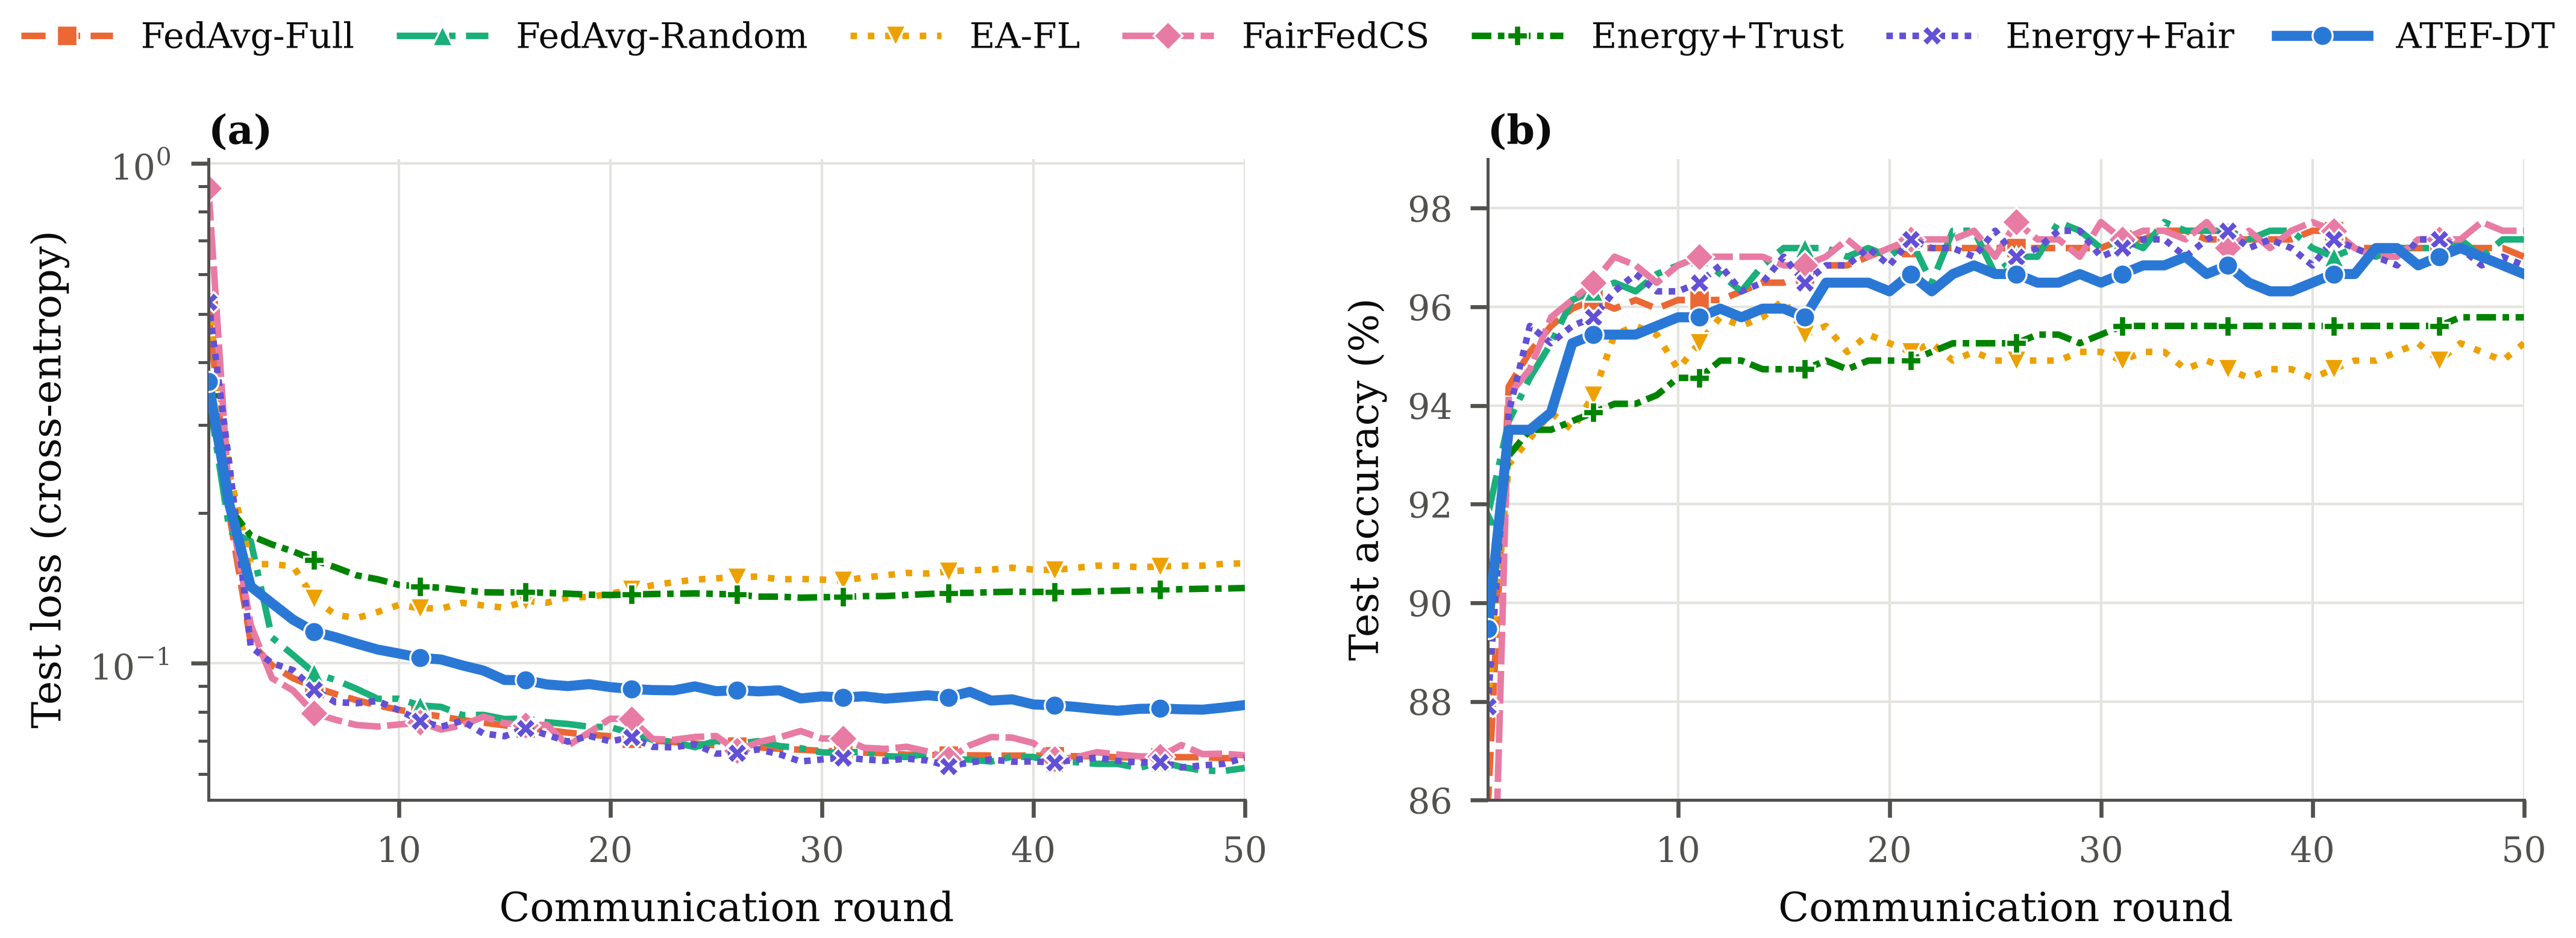
\includegraphics[width=\textwidth]{figures/fig_convergence}
	\revcap{R1.7(5), R1.7(6)}{Convergence on WDBC: (a)~test loss and (b)~test accuracy.}
	\label{fig:convergence}
\end{figure*}

\subsection{Energy and Traffic}
\label{subsec:energyres}
\rtag{R1.5}\begin{revblock}Table~\ref{tab:energy} and Figure~\ref{fig:energy} give the energy accounts. ATEF-DT consumes \Vpm{E-atef}{Esd-atef}~J. This is \V{sav-full}\% less than FedAvg-Full (\V{E-full}~J) and \V{sav-rand}\% less than FedAvg-Random (\V{E-rand}~J; paired $p=\V{p-E-atef-rand}$). The two figures answer different questions. FedAvg-Full has no budget and makes \V{tx-full} transmissions against 400, so most of the first saving is the effect of selecting eight clients per round: FedAvg-Random already saves \V{sav-rand-full}\% relative to FedAvg-Full. The comparison at equal budget is the one with FedAvg-Random. Of the \V{sav-rand}\% saved there, \V{Ecomp-sav-rand}~J come from computation, because the score prefers inexpensive clients among those that are under-served, and \V{Eul-sav-rand}~J from the uplink, because of quantization. EA-FL remains the least energy-consuming method at \V{E-eafl}~J. ATEF-DT spends \V{extra-eafl}\% more, which is the cost of spreading participation across clients; Section~\ref{subsec:fairres} shows what this buys in fairness.

\begin{table*}[t]
	\centering
	\revcap{R1.5}{Device energy (J) over 50 rounds and saving relative to FedAvg-Full and FedAvg-Random.}
	\label{tab:energy}
	\footnotesize
	\begin{tabular*}{\linewidth}{@{\extracolsep{\fill}}lccccccc}
		\toprule
		\textbf{Method} & \textbf{Computation} & \textbf{Uplink} & \textbf{Downlink} & \textbf{Signalling} & \textbf{Total} & \textbf{vs.\ Full (\%)} & \textbf{vs.\ Random (\%)} \\
		\midrule
		\tabin{tab_energy}
		\bottomrule
	\end{tabular*}
\end{table*}

\begin{figure*}[t]
	\centering
	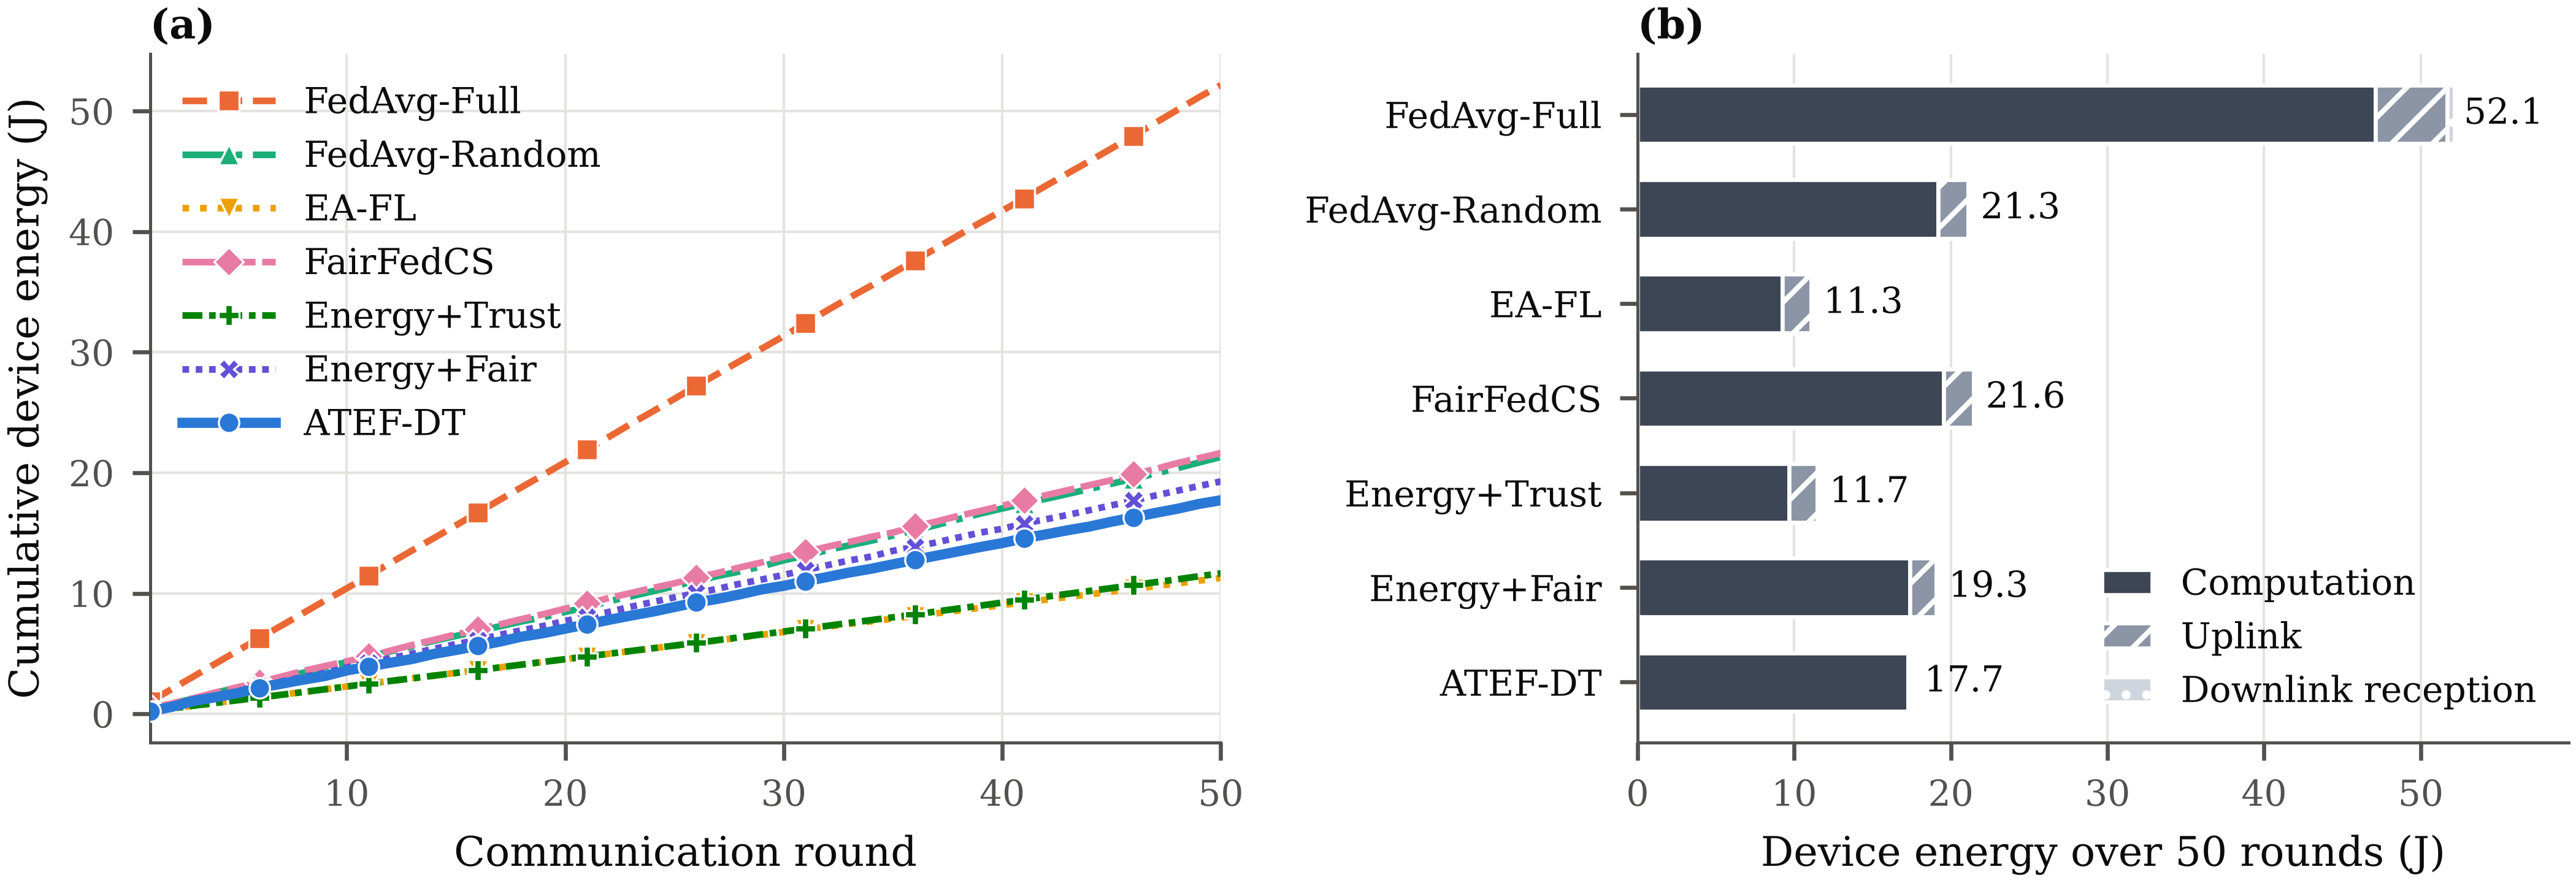
\includegraphics[width=\textwidth]{figures/fig_energy}
	\revcap{R1.5, R1.7(6)}{Device energy: (a)~cumulative energy and (b)~energy composition after 50 rounds.}
	\label{fig:energy}
\end{figure*}

\begin{table*}[t]
	\centering
	\revcap{R1.5}{Uplink traffic and energy of the bit-width policies under the ATEF-DT selection rule.}
	\label{tab:volume}
	\footnotesize
	\begin{tabular*}{\linewidth}{@{\extracolsep{\fill}}lccccccc}
		\toprule
		\textbf{Policy} & \textbf{Mean bits} & \textbf{Payload (Mb)} & \textbf{Metadata (Mb)} & \textbf{Uplink (Mb)} & \textbf{Reduction} & \textbf{Uplink energy (J)} & \textbf{Accuracy (\%)} \\
		\midrule
		\tabin{tab_volume}
		\bottomrule
	\end{tabular*}
\end{table*}

\begin{figure}[t]
	\centering
	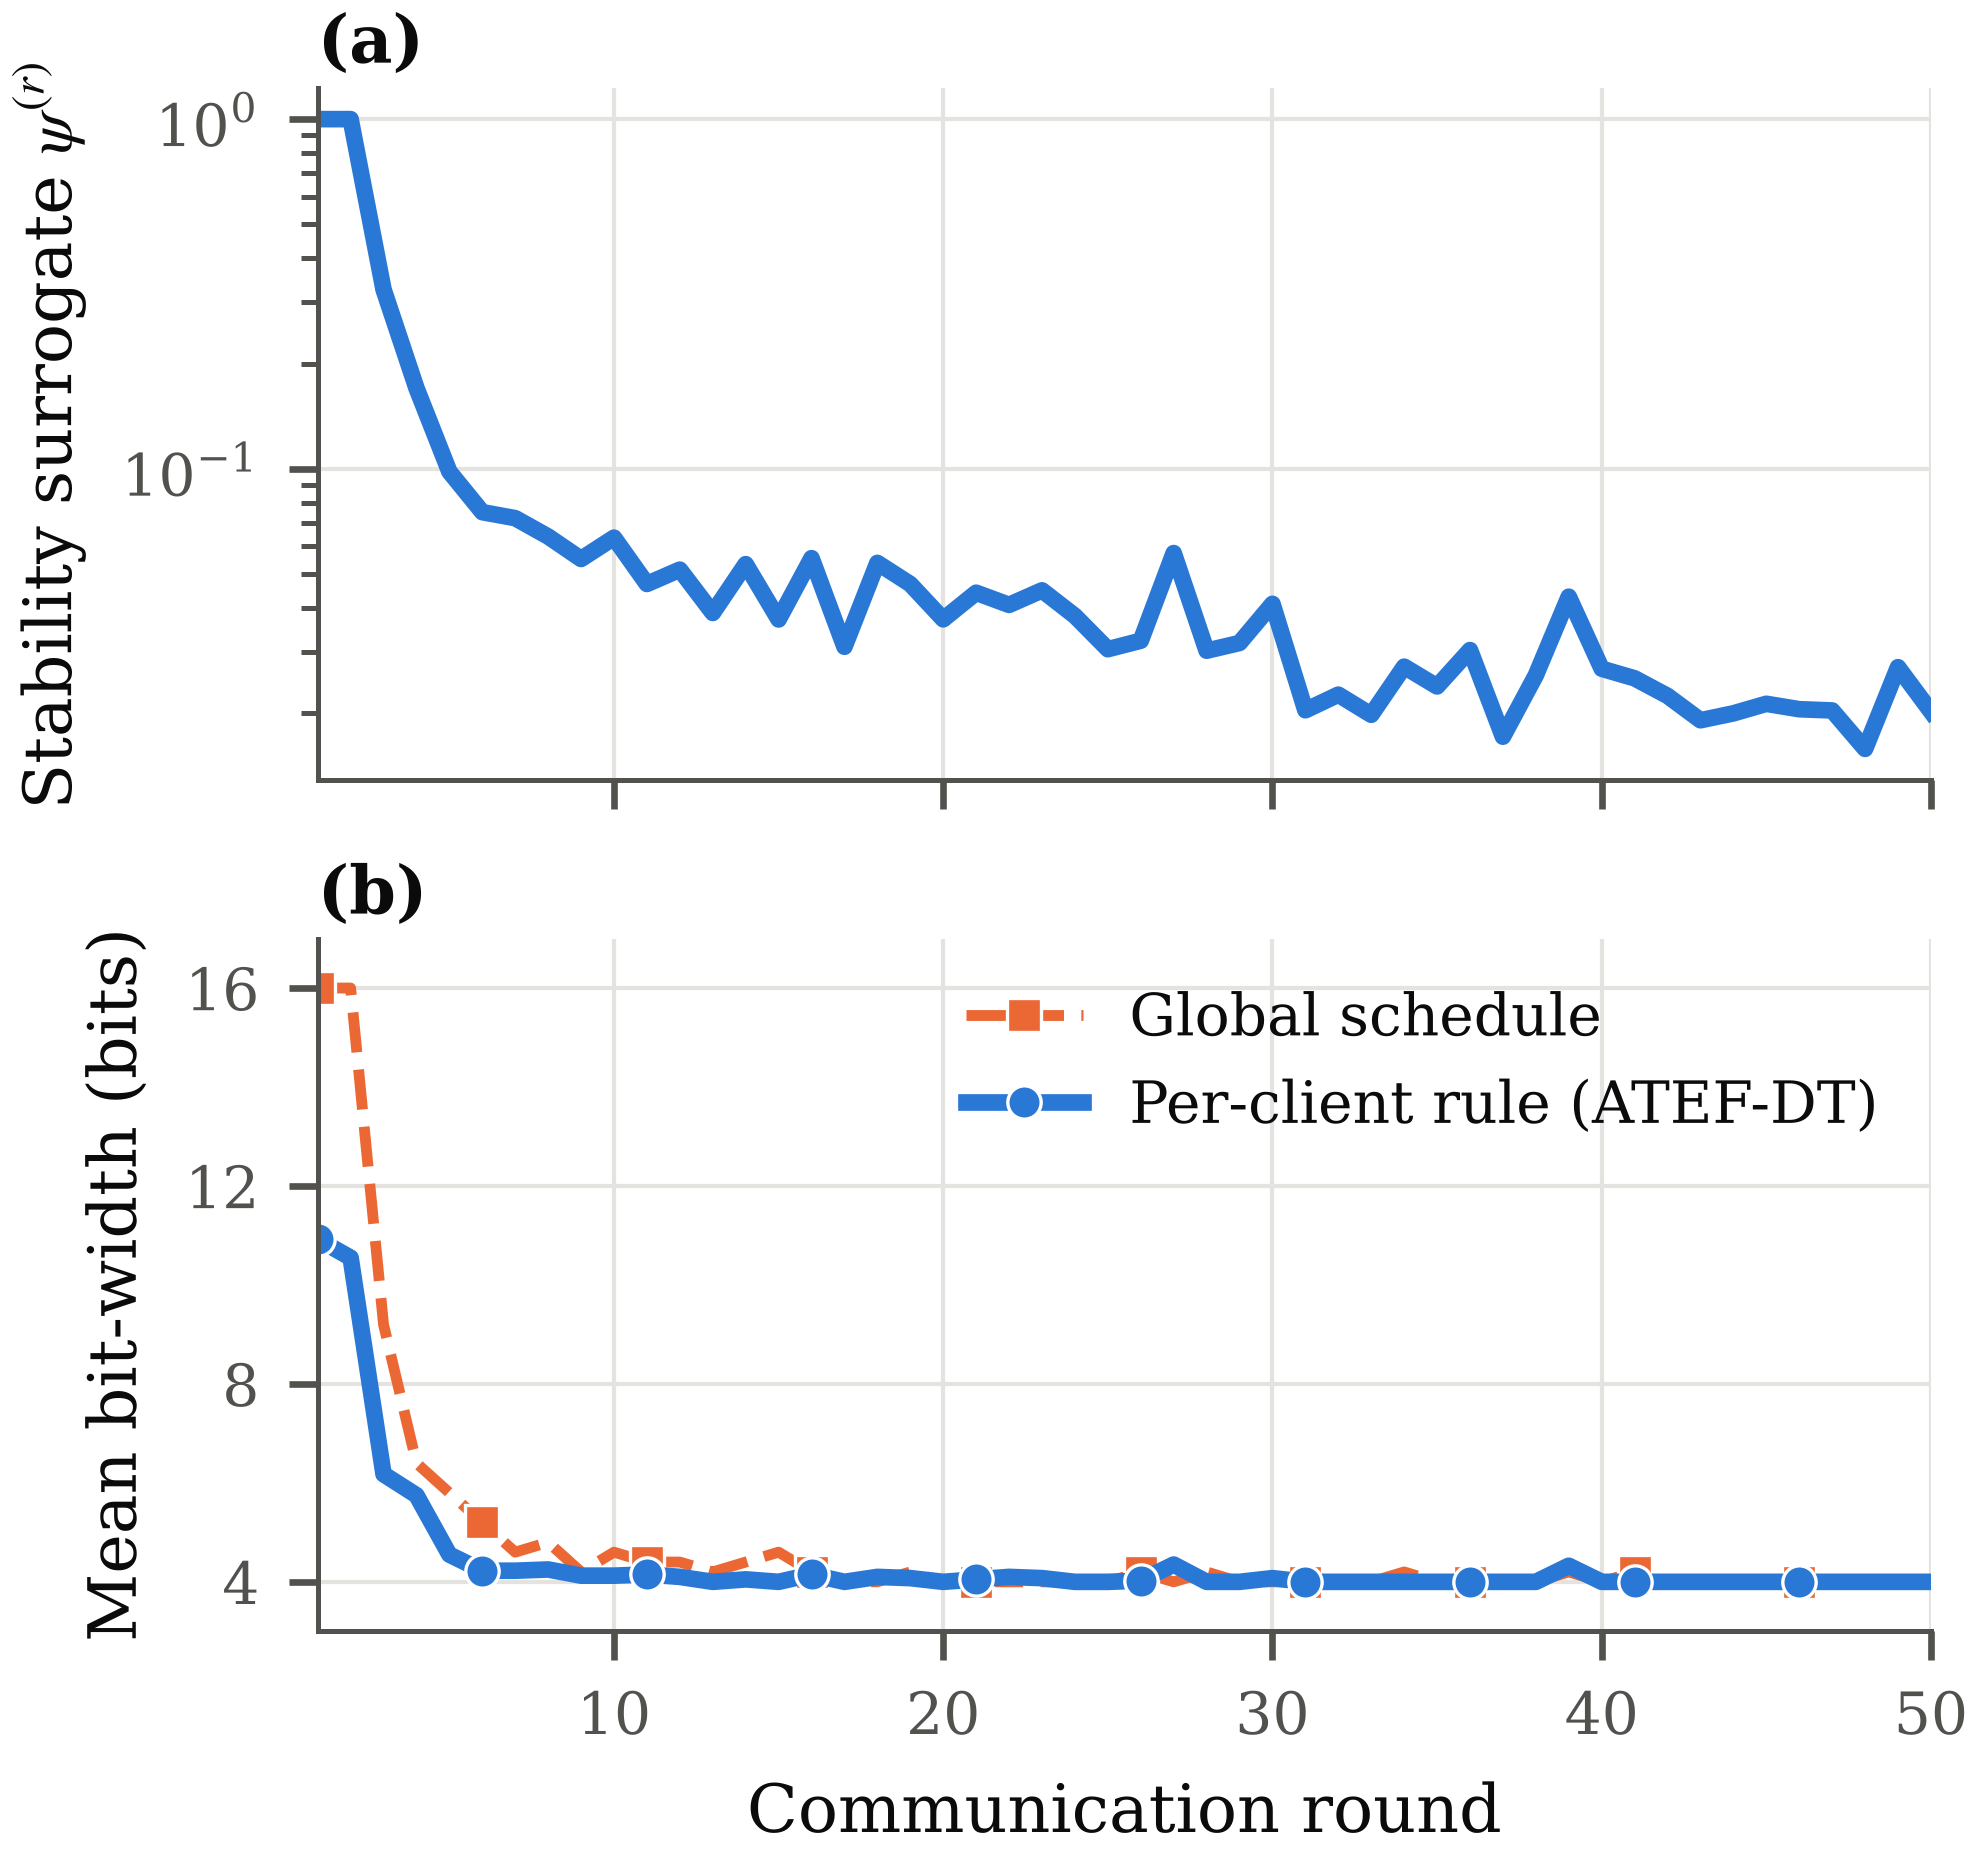
\includegraphics[width=\columnwidth]{figures/fig_bitwidth}
	\revcap{R1.7(1), R1.7(6)}{Adaptive quantization: (a)~stability surrogate $\psi^{(r)}$ and (b)~mean bit-width of the selected clients.}
	\label{fig:bitwidth}
\end{figure}

Computation dominates the account (\V{compshare-full}\% of the energy of FedAvg-Full), which is a consequence of the coefficient $\alpha$ of Table~\ref{tab:setup}. Section~\ref{subsec:sensitivity} varies $\alpha$ over three orders of magnitude; the default is the least favourable of the tested values for ATEF-DT.\end{revblock}

\rtag{R1.5}\begin{revblock}Table~\ref{tab:volume} compares four bit-width policies under the selection rule of ATEF-DT with full-precision transmission of the same updates. The per-client rule uses \V{meanb} bits per coordinate on average and reduces the uplink from \V{upMb-eftrust}~Mb to \V{upMb-atef2}~Mb, a factor of \V{compr}, in agreement with~\eqref{eq:compression}; the accuracy is unchanged within the variation across seeds. Figure~\ref{fig:bitwidth} shows why the mean is close to $b_{\min}$: the surrogate $\psi^{(r)}$ falls below $0.1$ within five rounds, after which nearly all transmissions use four bits. The reduction applies to the uplink only. The broadcast of the global model amounts to \V{downMb-atef}~Mb and the state reports to \V{stateMb}~Mb in every policy, so the total traffic falls from \V{totMb-eftrust}~Mb to \V{totMb-atef}~Mb, a reduction of \V{tot-red}\% and not of the \V{up-red}\% that the uplink alone would suggest.\end{revblock}

\subsection{Participation Fairness}
\label{subsec:fairres}
Figure~\ref{fig:fairness} shows the Jain index over the rounds. ATEF-DT reaches \Vpm{jain-atef}{jainsd-atef}, EA-FL \V{jain-eafl} and Energy+Trust \V{jain-etrust}; the latter two share the energy-greedy selection rule and return to the same clients. \rtag{R2.4}\rev{FedAvg-Random reaches \Vpm{jain-rand}{jainsd-rand}, in agreement with the expectation \V{jainexp} of~\eqref{eq:jainexp}; the small deficit is due to outages, which remove clients from some draws. The curve of FedAvg-Random in Figure~\ref{fig:fairness} follows the analytic curve throughout.} FedAvg-Full is below one (\V{jain-full}) for the same reason. FairFedCS reaches \V{jain-ffcs}: its queue grows in proportion to the reputation of a client, so it equalizes a reputation-weighted notion of fairness and not the raw participation counts that the Jain index measures.

\begin{figure}[t]
	\centering
	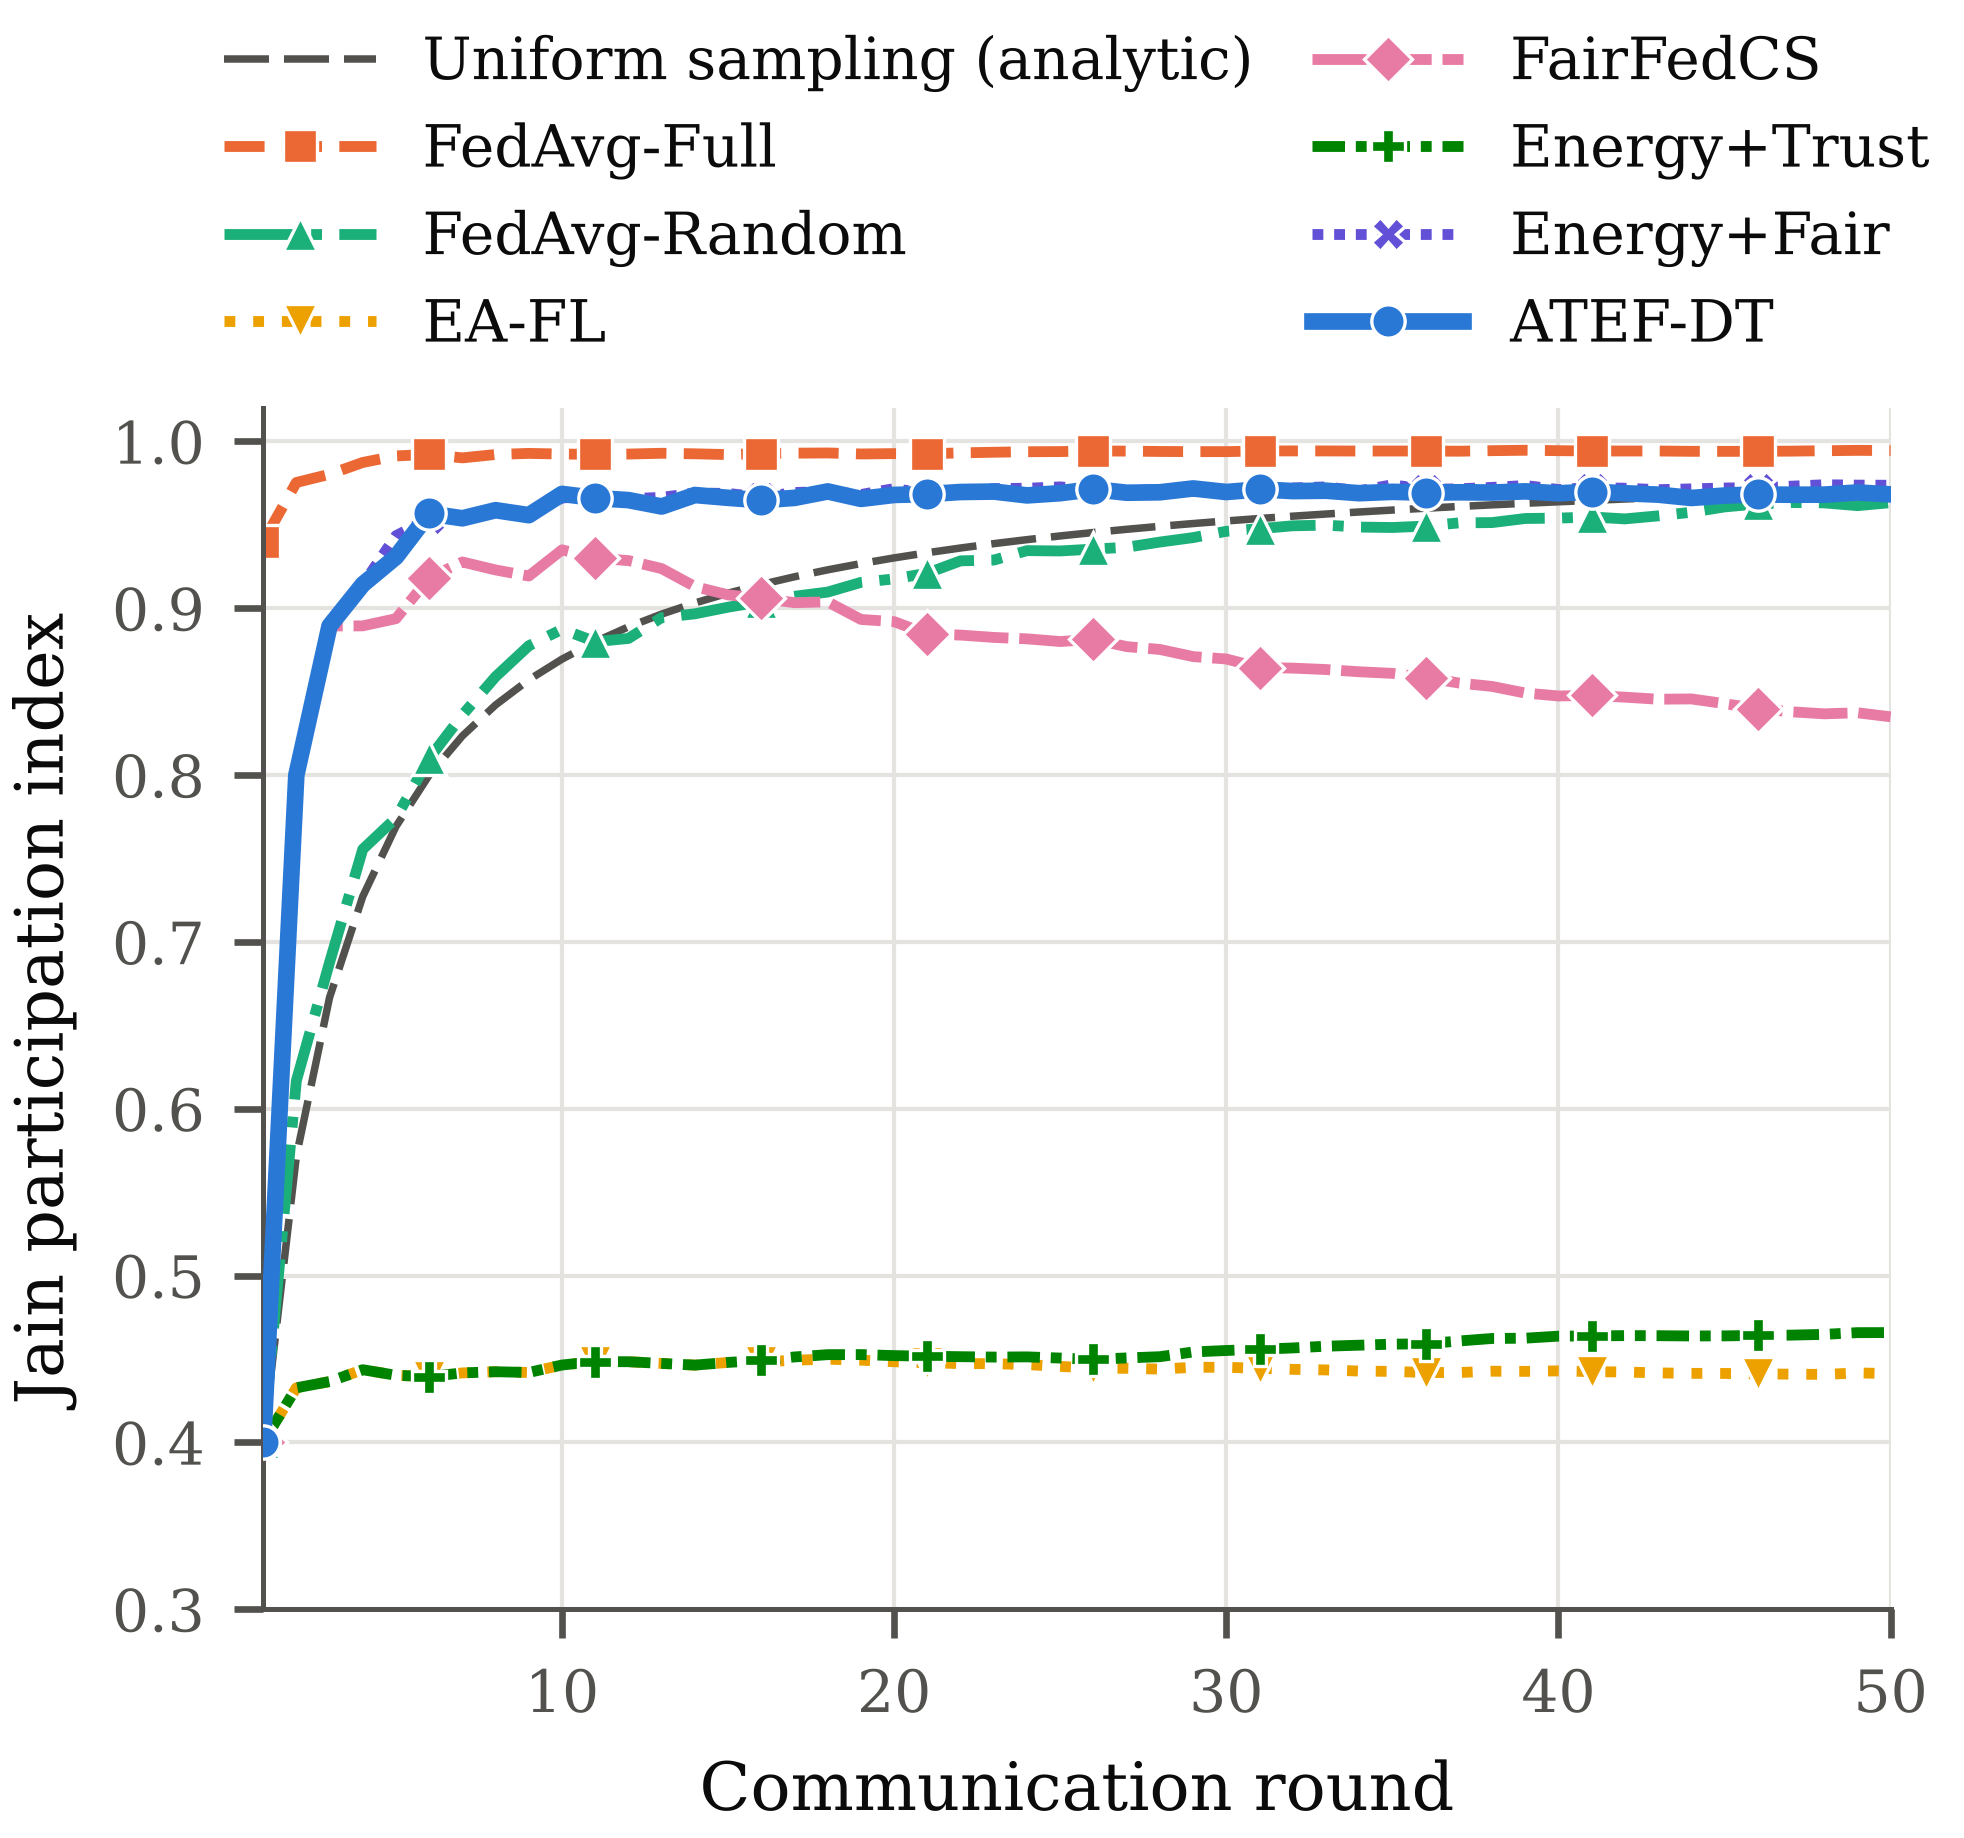
\includegraphics[width=\columnwidth]{figures/fig_fairness}
	\revcap{E4, R2.4}{Jain participation index; the dashed line is the expectation~\eqref{eq:jainexp} for uniform sampling.}
	\label{fig:fairness}
\end{figure}

\begin{table}[t]
	\centering
	\revcap{R1.5, E3}{Selection share and accuracy by device-resource tier, and distance of the effective weights from the data proportions.}
	\label{tab:group}
	\footnotesize
	\setlength{\tabcolsep}{2.5pt}
	\begin{tabular*}{\linewidth}{@{\extracolsep{\fill}}lccccc}
		\toprule
		 & \textbf{Share} & \multicolumn{2}{c}{\textbf{Accuracy (\%)}} & \textbf{Gap} & \\
		\cmidrule(lr){3-4}
		\textbf{Method} & \textbf{(\%)} & \textbf{High cost} & \textbf{Low cost} & \textbf{(pp)} & $\norm{\hat{\boldsymbol{\pi}}-\mathbf{n}/N}_1$ \\
		\midrule
		\tabin{tab_group}
		\bottomrule
	\end{tabular*}
\end{table}

\begin{figure*}[t]
	\centering
	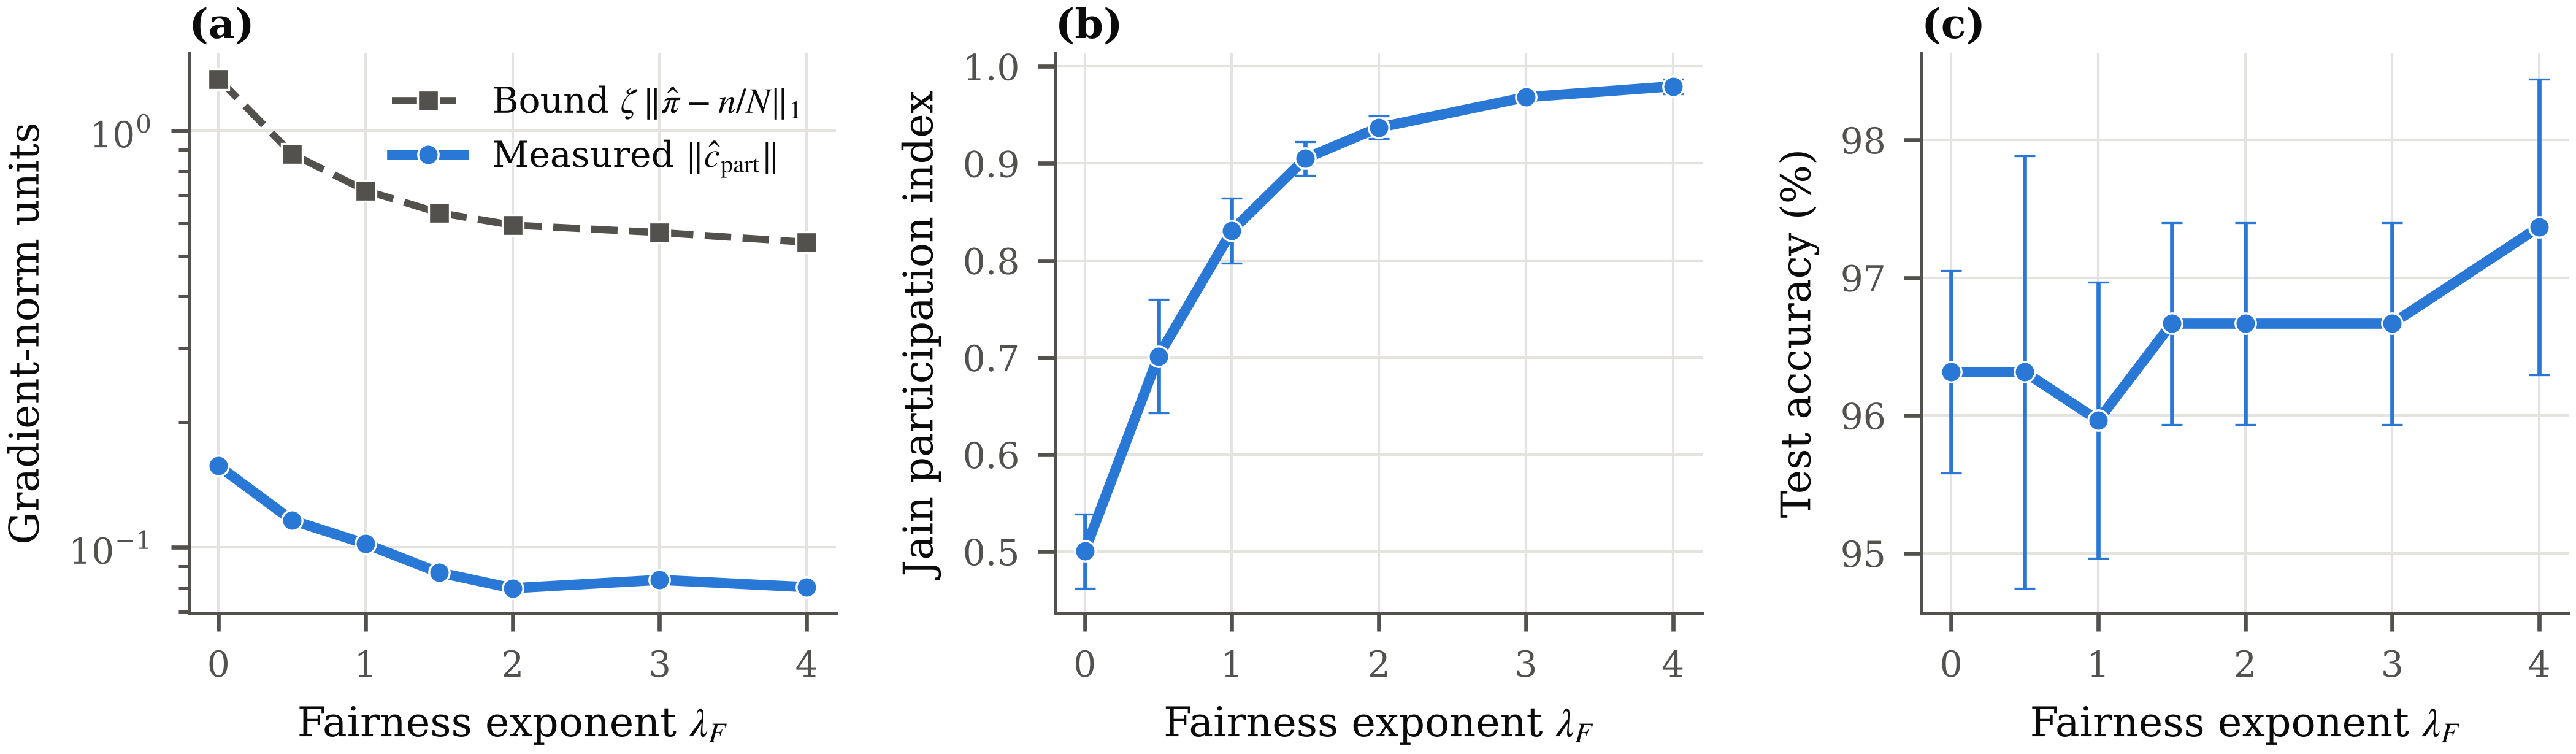
\includegraphics[width=\textwidth]{figures/fig_bias}
	\revcap{E3, R1.3, R2.3}{Effect of the fairness exponent $\lambda_F$: (a)~participation bias and its bound, (b)~Jain index and (c)~test accuracy.}
	\label{fig:bias}
\end{figure*}

\rtag{R1.5}\begin{revblock}The Jain index measures access to training. Whether unequal access harms the patients of the excluded devices is a separate question. To examine it, the clients are divided into two tiers by their static cost (computation energy plus full-precision uplink energy at the mean channel gain): a high-cost tier above the median and a low-cost tier below it. The test cases are assigned to clients with the class proportions of their training data, and accuracy is computed separately on the test cases of each tier. Table~\ref{tab:group} shows that EA-FL gives the high-cost tier \V{selhigh-eafl}\% of the selections and ATEF-DT \V{selhigh-atef}\%. The accuracy on the two tiers, however, differs by a few points at most for every method, with standard deviations of the same size, and EA-FL is not less accurate on the tier it excludes. On this data set, unequal participation does not translate into a consistent accuracy disparity between the tiers. The reason is that the features of WDBC are distributed similarly across clients, so a model trained on some clients serves the others. The fairness established here is therefore fairness of participation. WDBC contains no demographic or socio-economic attributes, and no claim is made about equity of outcomes for patient groups.\end{revblock}

\rtag{E3, R1.3, R2.3}\begin{revblock}Figure~\ref{fig:bias} varies $\lambda_F$ with the other exponents fixed. The Jain index rises from \V{jain-lf00} at $\lambda_F=0$ to \V{jain-lf40} at $\lambda_F=4$, and the energy from \V{E-lf00}~J to \V{E-lf40}~J. The accuracy stays between \V{acc-lf10}\% and \V{acc-lf40}\% without a trend that exceeds the variation across seeds. Panel~(a) reports the empirical counterpart of Proposition~\ref{prop:bias}: the effective weights are estimated by the run average $\hat{\boldsymbol{\pi}}=\sum_r\boldsymbol{\beta}^{(r)}/\sum_r s^{(r)}$, and the norm of $\sum_p(\hat\pi_p-N_p/N)\nabla f_p(\w^{(r)})$ and the bound $\zeta\norm{\hat{\boldsymbol{\pi}}-\mathbf{n}/N}_1$, with $\zeta$ the largest observed $\norm{\nabla f_p-\nabla F}$, are evaluated every ten rounds. The measured bias falls from \V{cpart-lf00} at $\lambda_F=0$ to \V{cpart-lf20} at $\lambda_F=2$ and is \V{cpart-lf30} at $\lambda_F=3$ and \V{cpart-lf40} at $\lambda_F=4$; it is not monotone, as anticipated in Section~\ref{subsec:bias}. The bound holds everywhere and is loose, by a factor of six to nine.

The last column of Table~\ref{tab:group} shows what the reputation weights cost. The distance of the effective weights from the data proportions is \V{pil1-efair} for Energy+Fair, which uses the same selection with data-volume weights, and \V{pil1-atef} for ATEF-DT. Most of the participation bias of ATEF-DT thus comes from the weighting and not from the selection. The measured step scale $s^{(r)}$ of ATEF-DT has a mean of \V{smean} and a minimum of \V{smin} over all rounds and seeds, well above the bound $\rho_{\min}/2$, so the condition $s_{\min}>0$ of Theorem~\ref{thm:convergence} is met in these runs.\end{revblock}

\subsection{Comparison With Multi-Objective Schedulers}
\label{subsec:schedulers}
\rtag{E1, R1.1, R2.1}\begin{revblock}This subsection tests the selection rule in isolation. Each of the five rules of Section~\ref{subsec:methods} has one parameter that trades energy against fairness: $\lambda_F$ for the weighted product and the weighted sum, $V$ for drift-plus-penalty, and the shortlist size $\bar k$ for the two pipelines. Each parameter is swept over a grid, and Figure~\ref{fig:frontier} shows the resulting energy--fairness curves, with FairFedCS, FedAvg-Random and EA-FL as single points. To compare the rules at equal fairness, a requirement of a Jain index of at least \V{jain-req} is imposed, and Table~\ref{tab:sched} reports, for each rule, the configuration on its grid that meets the requirement with the least energy.

\begin{figure}[t]
	\centering
	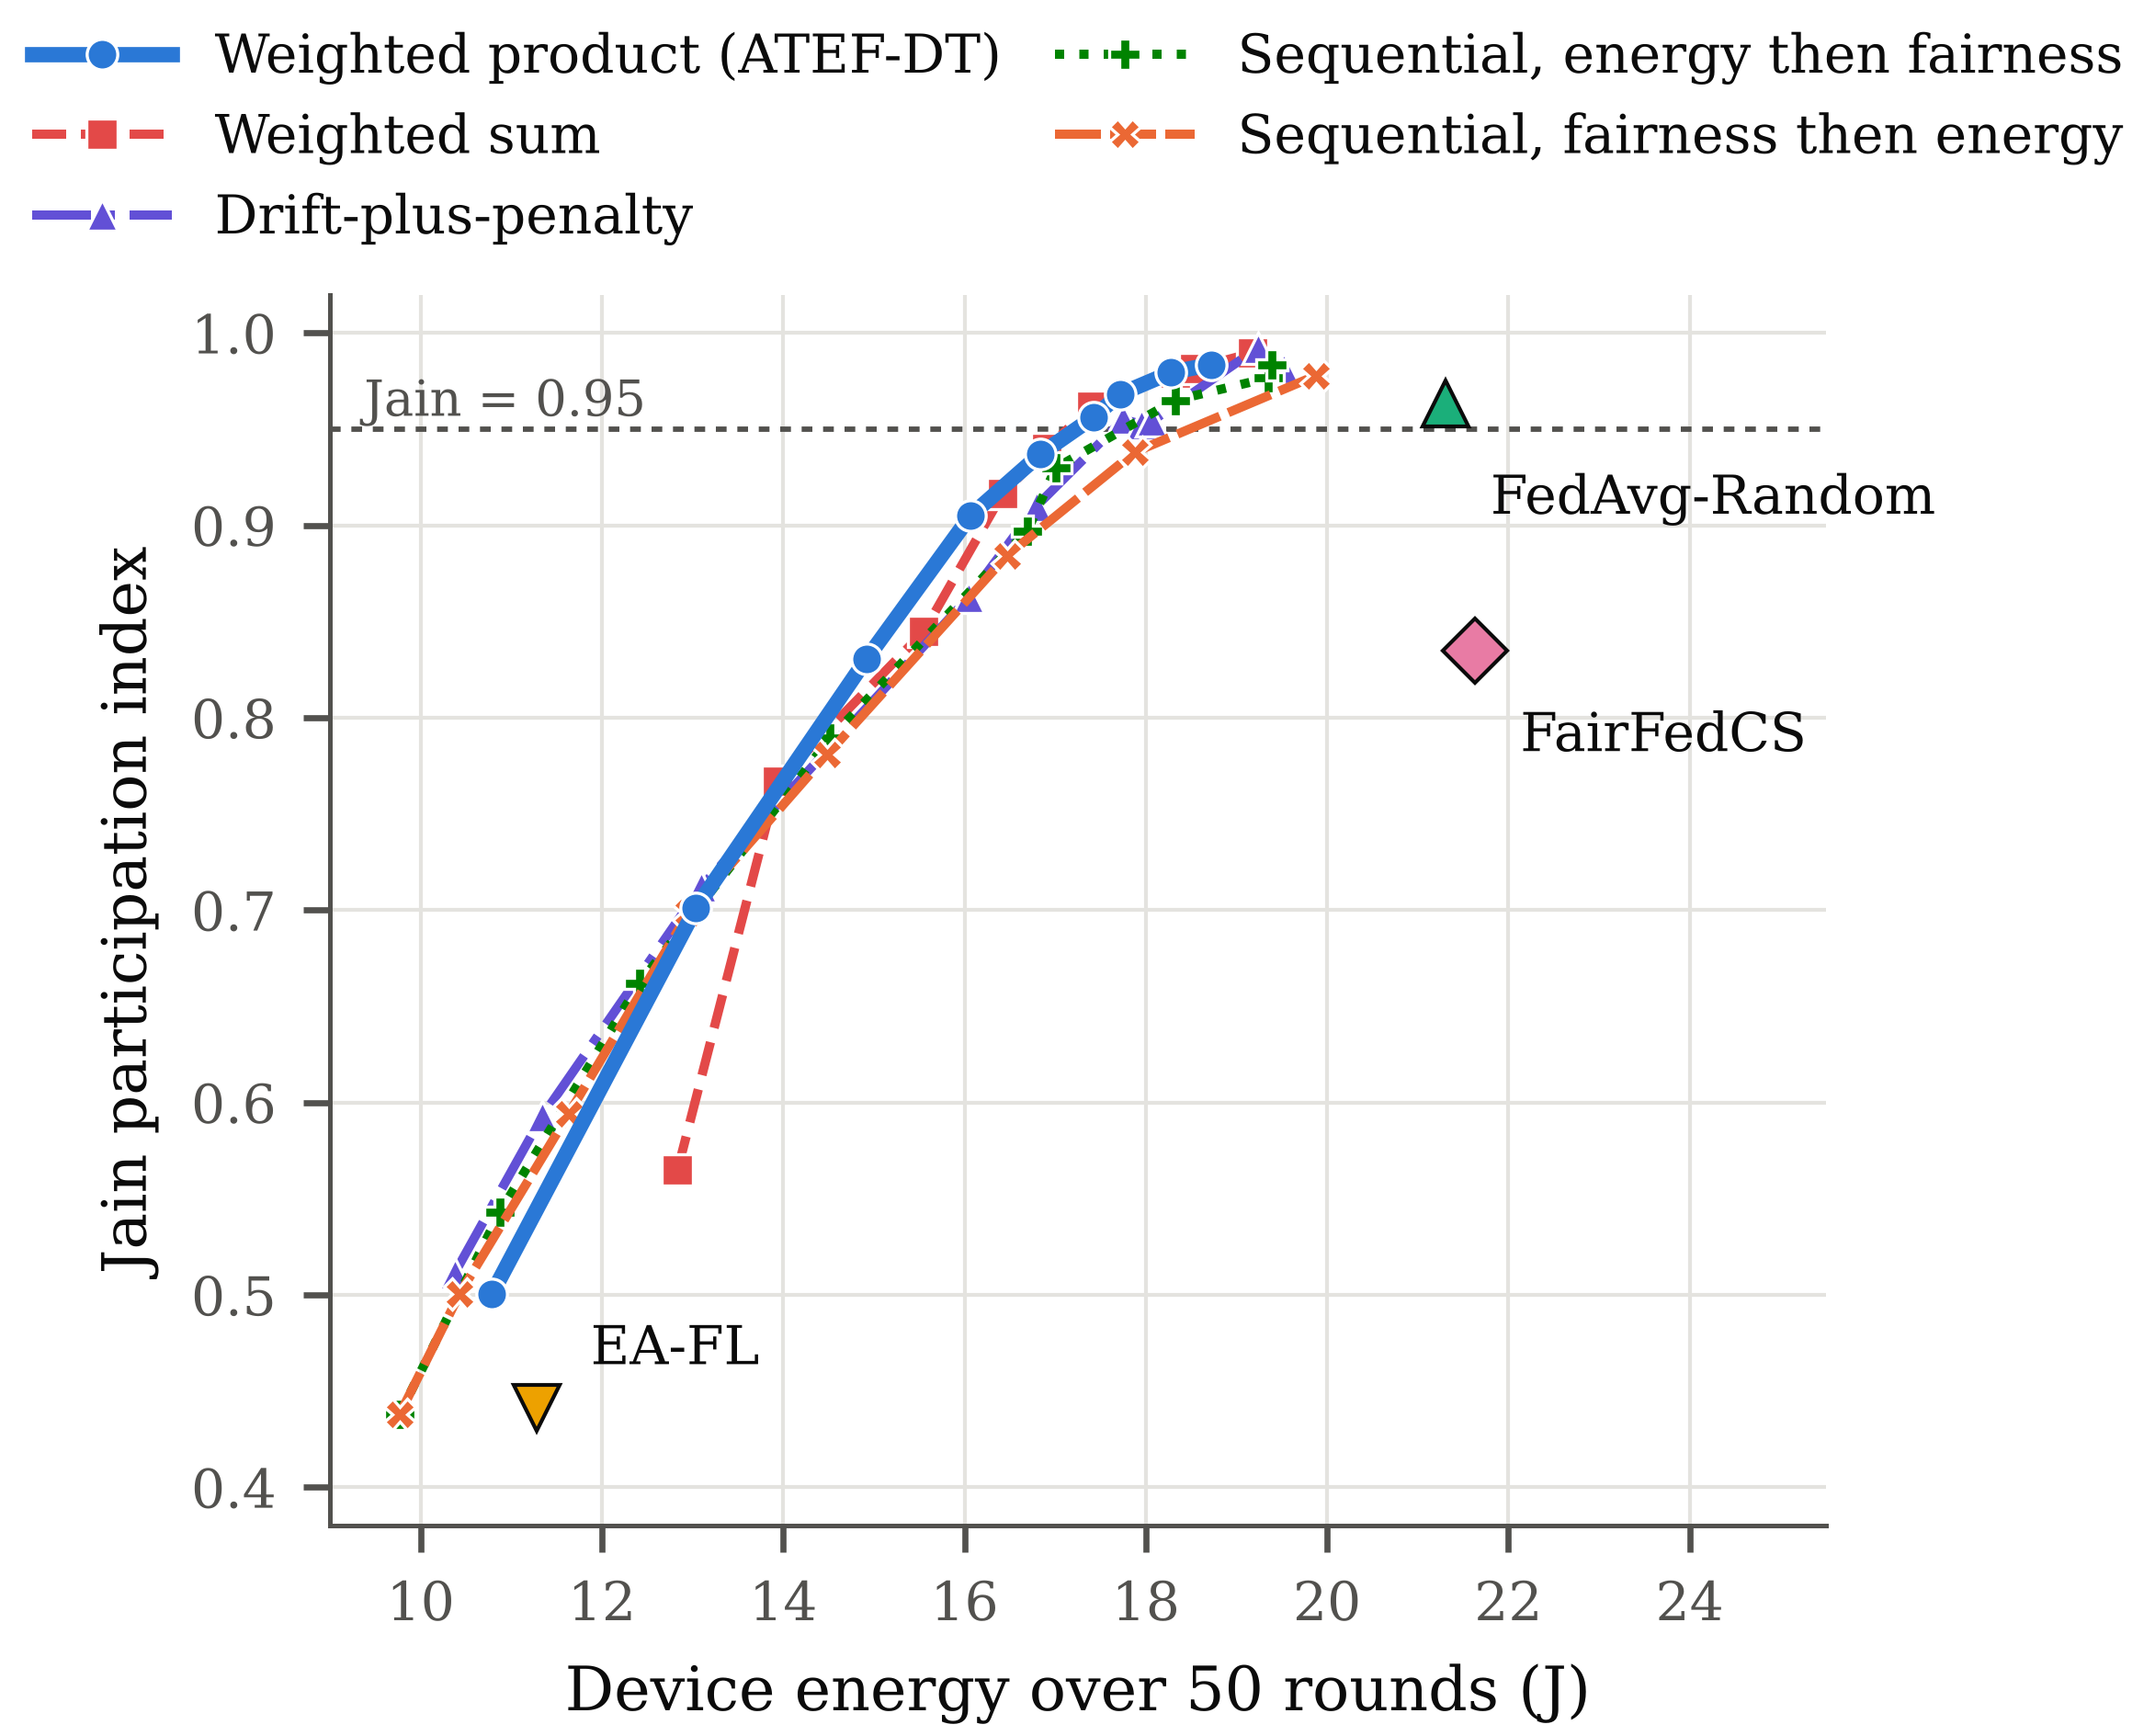
\includegraphics[width=\columnwidth]{figures/fig_frontier}
	\revcap{E1, R1.1, R2.1}{Energy--fairness curves of five selection rules.}
	\label{fig:frontier}
\end{figure}

\begin{table*}[t]
	\centering
	\revcap{E1, R1.1, R2.1}{Selection rules at a required Jain index of at least \V{jain-req}; the last column is the change in selections when the energy factor is scaled by $0.1$ / $10$.}
	\label{tab:sched}
	\footnotesize
	\begin{tabular*}{\linewidth}{@{\extracolsep{\fill}}llcccc}
		\toprule
		\textbf{Selection rule} & \textbf{Parameter} & \textbf{Jain index} & \textbf{Energy (J)} & \textbf{Accuracy (\%)} & \textbf{Change under rescaling (\%)} \\
		\midrule
		\tabin{tab_sched}
		\bottomrule
	\end{tabular*}
\end{table*}

Three findings follow. First, the three single-stage rules are indistinguishable. The weighted product needs \V{sched-E-prod}~J, the weighted sum \V{sched-E-add}~J and drift-plus-penalty \V{sched-E-dpp}~J; the paired differences to the weighted product are $\V{sched-diff-add}$~J ($p=\V{sched-p-add}$) and $\V{sched-diff-dpp}$~J ($p=\V{sched-p-dpp}$). At equal fairness, the weighted product is therefore as energy-efficient as a carefully tuned weighted sum. Second, the pipelines cost more. Seq-FE needs $\V{sched-diff-seqfe}$~J more than the weighted product ($p=\V{sched-p-seqfe}$); Seq-EF needs $\V{sched-diff-seqef}$~J more on average, a difference that is not significant over \V{nseeds} seeds ($p=\V{sched-p-seqef}$). Third, FairFedCS reaches a Jain index of \V{jain-ffcs} at \V{E-ffcs}~J: its index contains no energy term and its fairness notion is reputation-weighted, so it does not target this requirement.

The property that separates the weighted product from the weighted sum is Proposition~\ref{prop:scale}, and the last column of Table~\ref{tab:sched} measures it. When the energy factor is multiplied by $0.1$ or by $10$, with the exponents left at their default values, the selections of the weighted product do not change. Those of the weighted sum change by \V{resc-add-01}\% and \V{resc-add-10}\% of all selections, and under the factor $10$ its Jain index moves from \V{rescjain-add-1} to \V{rescjain-add-10} and its energy from \V{rescE-add-1}~J to \V{rescE-add-10}~J. A weighted sum therefore has to be re-tuned whenever the scale of a criterion changes, for instance with the hardware or the units, while the weighted product does not. This robustness to scaling, rather than a better energy--fairness trade-off, is the practical advantage of the product form.\end{revblock}

\subsection{Byzantine Robustness}
\label{subsec:byzantine}
Six attacks are simulated at adversarial fractions of 10\% to 40\% of the clients. \emph{Sign flipping} multiplies the update by $-1$; \emph{Gaussian poisoning} replaces it by a draw from $\mathcal{N}(\mathbf{0},(3\sigma_u)^2\mathbf{I})$, with $\sigma_u$ the root mean square of the honest update; \emph{label flipping} inverts the local labels before training; the \emph{scaled} attack multiplies the update by $10$; the \emph{backdoor} poisons half of the local samples with a trigger of four standard deviations on three features, targets the benign class and multiplies the update by $5$; and the \emph{adaptive} attack submits identical colluding updates at cosine $0.1$ to the mean honest update, along a common random direction and with the median honest norm. The adversaries are placed at random, independently for each seed, and attack from round~\V{attackstart}.

\begin{table}[t]
	\centering
	\caption{Test accuracy (\%) with 20\% adversarial clients.}
	\label{tab:byz}
	\footnotesize
	\begin{tabular*}{\linewidth}{@{\extracolsep{\fill}}lccc}
		\toprule
		\textbf{Method} & \textbf{No attack} & \textbf{Sign flipping} & \textbf{Label flipping} \\
		\midrule
		\tabin{tab_byz}
		\bottomrule
	\end{tabular*}
\end{table}

\begin{table*}[t]
	\centering
	\caption{Behaviour of the reputation layer of ATEF-DT under each attack with 20\% adversarial clients.}
	\label{tab:detail}
	\footnotesize
	\begin{tabular*}{\linewidth}{@{\extracolsep{\fill}}lccccccc}
		\toprule
		 & \textbf{Accuracy} & \textbf{Selection} & \textbf{Coefficient} & \textbf{Rejected} & \textbf{Adversaries} & \textbf{Honest} & \textbf{Success} \\
		\textbf{Attack} & \textbf{(\%)} & \textbf{share (\%)} & \textbf{share (\%)} & \textbf{(\%)} & \textbf{barred} & \textbf{barred (\%)} & \textbf{rate (\%)} \\
		\midrule
		\tabin{tab_detail}
		\bottomrule
	\end{tabular*}
\end{table*}

\begin{figure*}[t]
	\centering
	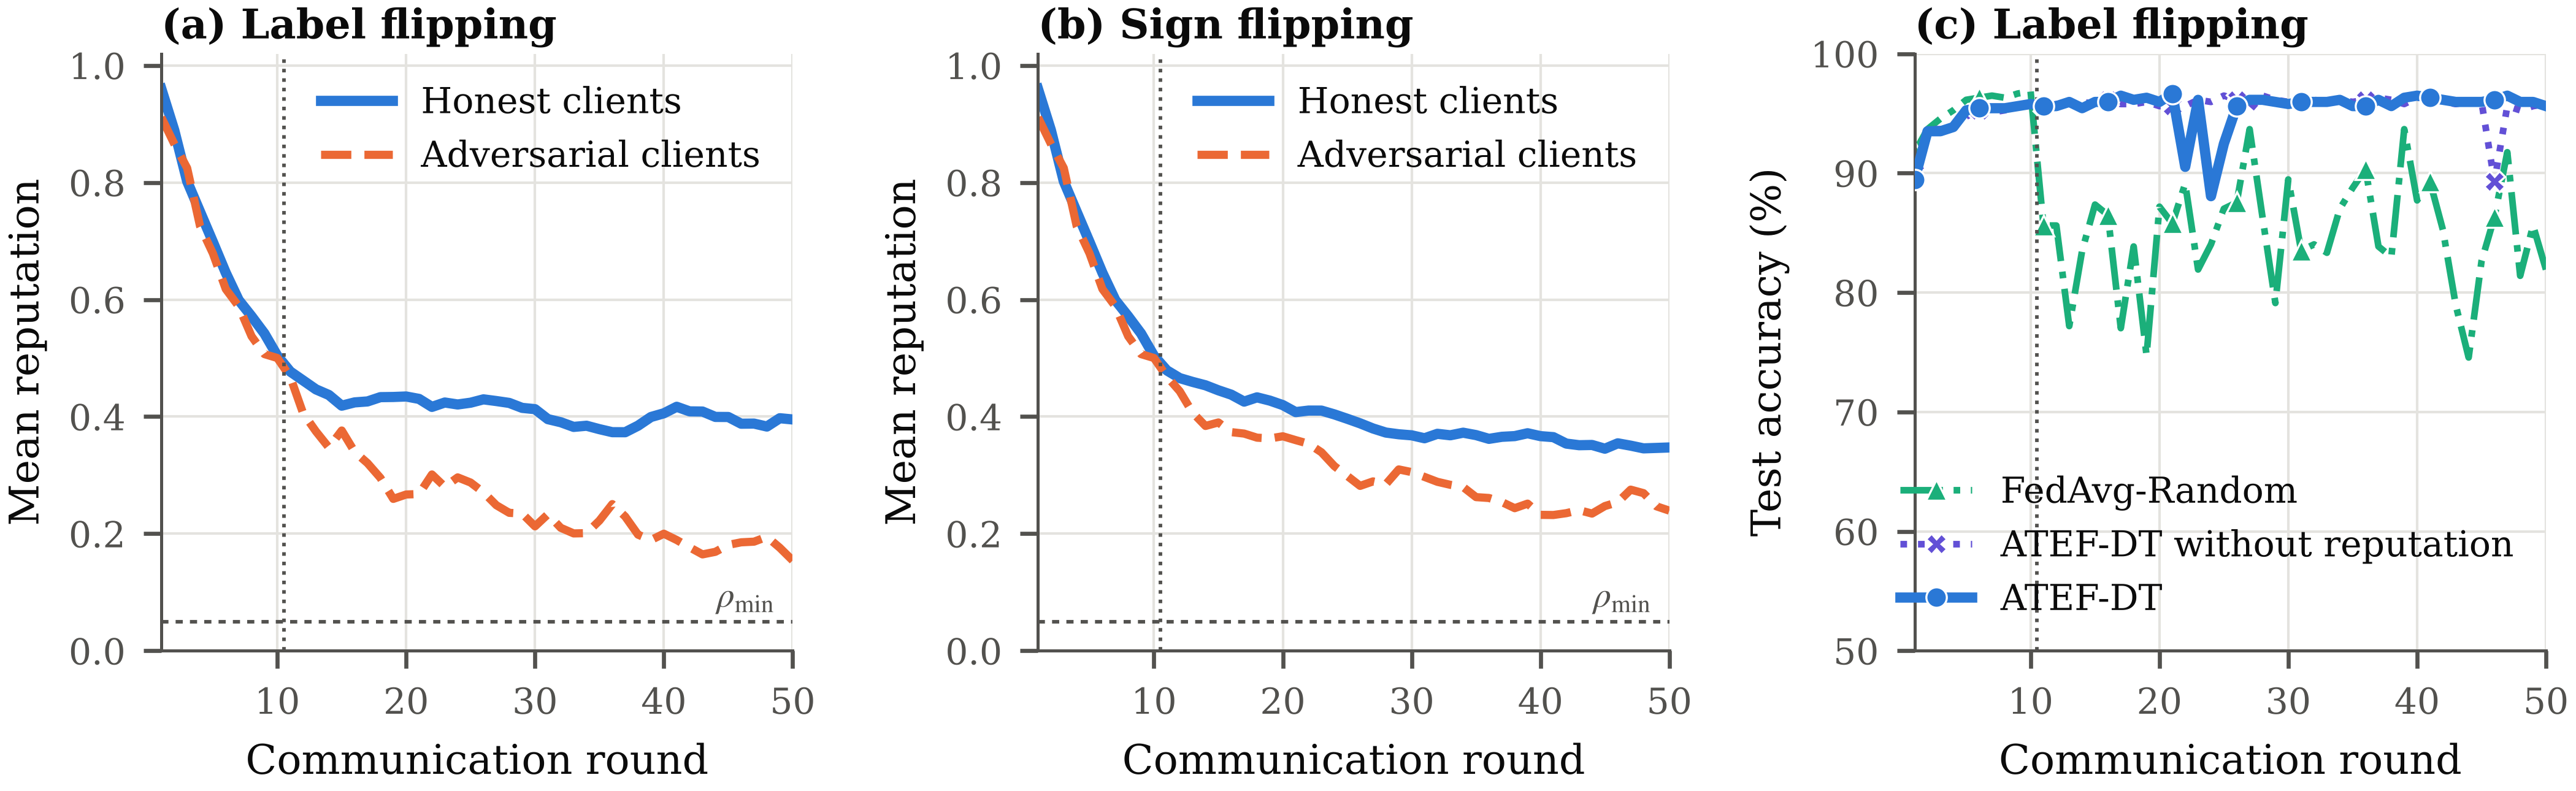
\includegraphics[width=\textwidth]{figures/fig_reputation}
	\revcap{R1.7(6)}{Reputations under (a)~label flipping and (b)~sign flipping, and (c)~accuracy under label flipping, with 20\% adversaries from round~\V{attackstart}.}
	\label{fig:reputation}
\end{figure*}

\begin{table*}[t]
	\centering
	\caption{Robust aggregation rules and matched variants.}
	\label{tab:robust}
	\footnotesize
	\begin{tabular*}{\linewidth}{@{\extracolsep{\fill}}lllccccc}
		\toprule
		 & & & \multicolumn{3}{c}{\textbf{Accuracy (\%)}} & \textbf{Energy} & \textbf{Jain} \\
		\cmidrule(lr){4-6}
		\textbf{Method} & \textbf{Selection} & \textbf{Aggregation} & \textbf{No attack} & \textbf{Sign flip} & \textbf{Label flip} & \textbf{(J)} & \textbf{index} \\
		\midrule
		\tabin{tab_robust}
		\bottomrule
	\end{tabular*}
\end{table*}

\begin{table}[t]
	\centering
	\caption{Test accuracy (\%) of ATEF-DT by attack and adversarial fraction.}
	\label{tab:grid}
	\footnotesize
	\setlength{\tabcolsep}{2.5pt}
	\begin{tabular*}{\linewidth}{@{\extracolsep{\fill}}lcccc}
		\toprule
		\textbf{Attack} & \textbf{10\%} & \textbf{20\%} & \textbf{30\%} & \textbf{40\%} \\
		\midrule
		\tabin{tab_grid}
		\bottomrule
	\end{tabular*}
\end{table}

\begin{table}[t]
	\centering
	\caption{Realized adversarial share of the selected set and rounds violating Assumption~\ref{ass:threat}.}
	\label{tab:realized}
	\footnotesize
	\begin{tabular*}{\linewidth}{@{\extracolsep{\fill}}ccc}
		\toprule
		\textbf{Adversarial} & \textbf{Mean share of the} & \textbf{Rounds violating} \\
		\textbf{clients (\%)} & \textbf{selected set (\%)} & \textbf{Assumption~\ref{ass:threat} (\%)} \\
		\midrule
		\tabin{tab_realized}
		\bottomrule
	\end{tabular*}
\end{table}

\begin{table}[t]
	\centering
	\caption{Test accuracy (\%) with 30\% and 40\% adversarial clients.}
	\label{tab:high}
	\footnotesize
	\setlength{\tabcolsep}{2pt}
	\begin{tabularx}{\columnwidth}{>{\raggedright\arraybackslash}X cccc}
		\toprule
		 & \multicolumn{2}{c}{\textbf{Sign flipping}} & \multicolumn{2}{c}{\textbf{Label flipping}} \\
		\cmidrule(lr){2-3}\cmidrule(lr){4-5}
		\textbf{Method} & \textbf{30\%} & \textbf{40\%} & \textbf{30\%} & \textbf{40\%} \\
		\midrule
		\tabin{tab_high}
		\bottomrule
	\end{tabularx}
\end{table}

\begin{table*}[t]
	\centering
	\caption{Sensitivity of the reputation layer to $\mu$ and $\rho_{\min}$ (default marked with an asterisk).}
	\label{tab:trustsens}
	\footnotesize
	\begin{tabular*}{\linewidth}{@{\extracolsep{\fill}}cccccccc}
		\toprule
		 & & & \textbf{Honest barred,} & \textbf{Accuracy} & \textbf{Coefficient} & \textbf{Adversaries} & \textbf{Honest} \\
		$\boldsymbol{\mu}$ & $\boldsymbol{\rho_{\min}}$ & $\boldsymbol{k^{\star}}$ & \textbf{no attack (\%)} & \textbf{(\%)} & \textbf{share (\%)} & \textbf{barred} & \textbf{barred (\%)} \\
		\midrule
		\tabin{tab_trustsens}
		\bottomrule
	\end{tabular*}
\end{table*}

\begin{table*}[t]
	\centering
	\revcap{E4, R1.7(2)}{Functional test of the twin layer with synthetic streams and small batteries.}
	\label{tab:twin}
	\footnotesize
	\begin{tabular*}{\linewidth}{@{\extracolsep{\fill}}lccccc}
		\toprule
		\textbf{Feasibility screen} & \textbf{Reserve breaches} & \textbf{Client-rounds with} & \textbf{Transmissions} & \textbf{Jain index} & \textbf{Accuracy (\%)} \\
		 & \textbf{after participation} & \textbf{empty battery} & & & \\
		\midrule
		\tabin{tab_twin}
		\bottomrule
	\end{tabular*}
\end{table*}

Table~\ref{tab:byz} compares the methods under sign flipping and label flipping. Label flipping is the more damaging attack in this setting: FedAvg-Random falls to \Vpm{lf20-rand}{lf20sd-rand}\% and EA-FL to \V{lf20-eafl}\%, while ATEF-DT retains \Vpm{lf20-atef}{lf20sd-atef}\% (paired $p=\V{p-lf-atef-rand}$ against FedAvg-Random; the large spread of the baseline across seeds limits the power of the test). Under sign flipping the methods are closer (\V{sf20-rand}\% for FedAvg-Random, \V{sf20-atef}\% for ATEF-DT), because a flipped full-batch gradient of a minority only shortens the average step.

Table~\ref{tab:detail} reports the behaviour of the reputation layer for each attack at 20\%, and Figure~\ref{fig:reputation} shows the reputations over time. Under label flipping the adversaries receive \V{g-malsel-lf20}\% of the selections but carry only \V{g-malw-lf20}\% of the aggregation coefficients: their reputation falls and the weights~\eqref{eq:agg} follow. The gate plays a minor part. Only \V{g-bar-lf20} of \V{g-nadv-lf20} adversaries are barred within the run, and \V{g-rej-lf20}\% of the received malicious updates are rejected. The exclusion time $k^{\star}=\V{kstar}$ of Lemma~\ref{lem:rep} is rarely attained, because its premise, a trust signal that is never positive, does not hold: each received update is itself part of the set from which the reference is computed, which gives every update a positive alignment with the reference, of the order of $1/\sqrt{k}$ for $k$ otherwise uncorrelated updates of comparable norm, and as training approaches a stationary point the honest updates lose their common direction, so the signal no longer separates the two populations. Figure~\ref{fig:reputation} shows this: the mean reputation of honest clients settles near $0.4$, not near one, and that of the adversaries declines slowly. The reputation layer thus acts through graded weights and not through exclusion. In clean runs it bars \V{fe-clean}\% of the honest clients, and such an exclusion is permanent.

Table~\ref{tab:robust} places ATEF-DT beside four robust aggregation rules and beside its own variants without the reputation layer. At 20\% adversaries the methods are close. The variant that keeps the clipping and replaces the reputation weights by an unweighted mean reaches \V{lf20-norep}\% under label flipping and \V{sf20-norep}\% under sign flipping, against \V{lf20-atef}\% and \V{sf20-atef}\% for ATEF-DT ($p=\V{p-lf-atef-norep}$ for label flipping), and the geometric median with uniform selection reaches \V{lf20-gm}\% and \V{sf20-gm}\%. At this adversarial fraction, clipping accounts for most of the robustness of ATEF-DT, and the reputation weights add no measurable accuracy. What ATEF-DT offers over the robust aggregation baselines is the same robustness at lower energy (\V{E-atef}~J against \V{E-rand}~J), since those baselines select uniformly at full precision.

Table~\ref{tab:grid} gives the accuracy of ATEF-DT for all attacks and fractions, and Table~\ref{tab:realized} the realized composition of the selected sets. Up to 20\% the accuracy stays within 1.3 points of the clean value for every attack. At 30\% it holds under label flipping (\V{g-acc-lf30}\%) and becomes unstable under sign flipping (\Vpm{g-acc-sf30}{g-accsd-sf30}\%). At 40\% the method fails under both (\V{g-acc-sf40}\% and \V{g-acc-lf40}\%). The failure has a definite cause: with 40\% adversarial clients, adversaries are at least half of the selected set in \V{viol-40}\% of the rounds, which violates Assumption~\ref{ass:threat}; in such rounds the reference is captured, the adversaries gain reputation and the honest clients lose it, and the reputations carry the error into later rounds. Table~\ref{tab:high} shows the consequence. Beyond the domain of Assumption~\ref{ass:threat} the memory of the reputation layer is a liability: under sign flipping at 40\%, ATEF-DT (\V{hi-sf40-dt}\%) is far below its own variant without reputation (\V{hi-sf40-norep}\%) and below the geometric median (\V{hi-sf40-gm}\%), whereas under label flipping at 30\% it is above both.

Against the backdoor the protection is partial. With 20\% adversaries the attack success rate is \V{g-asr-bd20}\% for ATEF-DT, against \V{asr20-rand}\% for FedAvg-Random; at 10\% it is \V{g-asr-bd10}\%. The variant without reputation (\V{asr20-norep}\%) and the geometric median (\V{asr20-gm}\%) do at least as well, so the reduction is due to clipping and the reputations do not contribute to it. The clean accuracy is hardly affected by the backdoor, which would therefore not be noticed from the accuracy. The adaptive adversary exposes the second part of Assumption~\ref{ass:threat}. Its colluders submit identical vectors at a small positive cosine to the honest mean. Identical vectors attract the geometric median, the colluders are then closer to the reference than the honest clients, and the engine rewards them: at 20\% they receive \V{g-malsel-ad20}\% of the selections and \V{g-malw-ad20}\% of the aggregation coefficients, and at 40\% they hold \V{g-malw-ad40}\% of the coefficients while \V{g-fe-ad40}\% of the honest clients are barred. The accuracy remains high in Table~\ref{tab:grid} only because the direction that this adversary injects is random and not chosen to increase the loss. Against colluding clients the credibility engine does not protect the model.

Table~\ref{tab:trustsens} varies the forgetting factor and the threshold. Raising the threshold to $0.10$ bars more adversaries and many honest clients; a longer memory ($\mu=0.8$) bars almost none of either. The share of the coefficients carried by label-flipping adversaries stays below three per cent in all configurations, and the accuracy is 95\% or higher in all but one. These observations confirm that the weights, and not the gate, carry the protection, and that the gate could be removed at little cost. When the attack starts at round~0 instead of round~\V{attackstart}, the accuracy under label flipping is \V{on0-lf-acc}\% and under sign flipping \V{on0-sf-acc}\%. A variant in which the reference~\eqref{eq:gm} is weighted by the reputations was examined and rejected: it couples the reference to its own output, and in clean runs it barred \V{wref-fe}\% of the honest clients and lowered the Jain index to \V{wref-jain}. It remains available as an option in the released code.

\rtag{E4, R1.5, R1.7(2)}\begin{revblock}WDBC has no physiological stream, and with the batteries of Table~\ref{tab:setup} the screen~\eqref{eq:screen} never binds. The twin layer is therefore tested on its own, with synthetic streams and small batteries; the learning task is unchanged. Each patient has $m=3$ standardized vital-sign deviations that follow a mean-reverting process, and half of the patients undergo a deterioration episode during the run, in which the mean rises over eight rounds to between $0.75$ and $4$ standard deviations depending on the variable. Measurements carry Gaussian noise of standard deviation $\V{twc-twinrsd}$ and are missing in 20\% of the rounds. The batteries are drawn uniformly from $[\V{twc-batterylow},\V{twc-batteryhigh}]$~J, with a reserve of \V{twc-Cres}~J and $C_{\mathrm{ref}}=\V{twc-Cref}$~J. The streams are generated by a model that differs from the twin model~\eqref{eq:twinmodel}, so that the twin is not tested on data from its own model class.

Table~\ref{tab:twin} compares three screens: the twin forecast~\eqref{eq:screen}, an instantaneous test $C_p^{(r)}-\hat e_p^{(r)}\ge C_{\mathrm{res}}$, and no reserve. The first column counts the participations that are followed, within $H$ rounds, by a fall of the battery below the reserve. The twin forecast reduces these events from \V{tw-breach-none} to \V{tw-breach-twin} per run, against \V{tw-breach-instant} for the instantaneous test, and it reduces the client-rounds with an empty battery. It does so by withdrawing devices earlier, which lowers the Jain index from \V{tw-jain-none} to \V{tw-jain-twin} and the accuracy from \V{tw-acc-none}\% to \V{tw-acc-twin}\%. The screen thus trades participation for monitoring continuity, as intended, and it does not remove the events entirely, because an episode that starts after a participation cannot be foreseen.

The tracking error shows what the filter contributes. The mean absolute error of the local-level twin is \V{tw-mae-level} standardized units, against \V{tw-mae-hold} when the last received measurement is held and \V{tw-mae-ar} for the autoregressive alternative. The advantage of filtering grows with the sensor noise: at a noise of $0.40$ the errors are \V{tw-mae-level-04} and \V{tw-mae-hold-04}, and at $0.10$ they are \V{tw-mae-level-01} and \V{tw-mae-hold-01}, so that with accurate sensors holding the last measurement is almost as good. The autoregressive model, fitted on a resting window, reverts to rest during an episode and is not better than holding at low noise (\V{tw-mae-ar-01}); this is the reason for adopting the local-level model. These results establish that the twin layer functions as specified on synthetic data. They do not establish its clinical validity.\end{revblock}

\subsection{Ablation}
\label{subsec:ablation}
Table~\ref{tab:ablation} and Figure~\ref{fig:ablation} add the components one at a time. The fairness factor (C1 to C2) raises the Jain index from \V{jain-eafl} to \V{jain-efair} and the energy from \V{E-eafl}~J to \V{E-efair}~J. The reputation layer (C2 to C3) leaves energy and fairness essentially unchanged, lowers the clean accuracy slightly, from \V{acc-efair}\% to \V{acc-eftrust}\%, and raises the accuracy under label flipping from \V{lf20-efair}\% to \V{lf20-eftrust}\%; as shown in Section~\ref{subsec:byzantine}, most of this gain is due to clipping. Adaptive quantization (C3 to C4) reduces the uplink from \V{upMb-eftrust}~Mb to \V{upMb-atef}~Mb and the energy to \V{E-atef}~J without loss of accuracy.

\begin{table*}[t]
	\centering
	\caption{Ablation of ATEF-DT; each row adds one component to the previous one.}
	\label{tab:ablation}
	\footnotesize
	\begin{tabular*}{\linewidth}{@{\extracolsep{\fill}}lccccc}
		\toprule
		\textbf{Configuration} & \textbf{Accuracy (\%)} & \textbf{Energy (J)} & \textbf{Jain index} & \textbf{Uplink (Mb)} & \textbf{Label flip (\%)} \\
		\midrule
		\tabin{tab_ablation}
		\bottomrule
	\end{tabular*}
\end{table*}

\begin{figure*}[t]
	\centering
	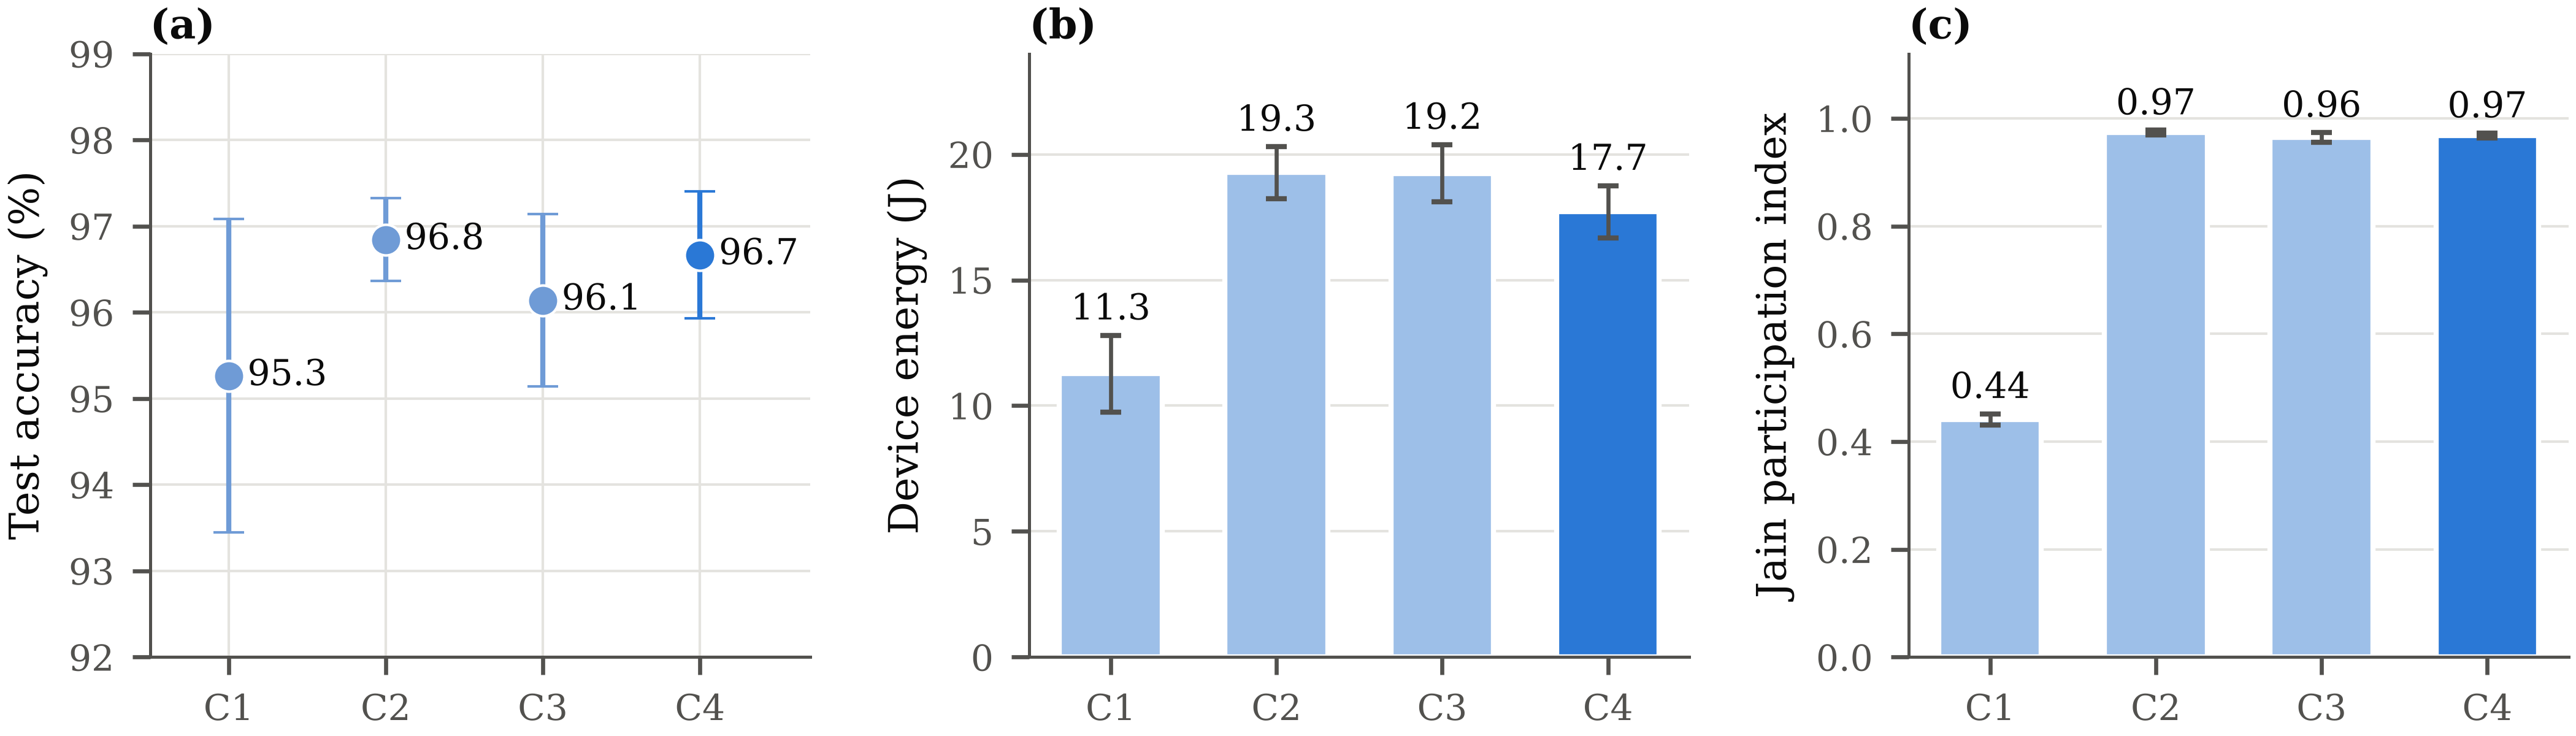
\includegraphics[width=\textwidth]{figures/fig_ablation}
	\revcap{R1.7(6)}{Ablation: (a)~test accuracy, (b)~device energy and (c)~Jain index.}
	\label{fig:ablation}
\end{figure*}

\subsection{Scalability and Overhead}
\label{subsec:scalability}
The population is increased from 20 to \V{pmax} clients with the budget kept at 40\% of the clients. Since WDBC is small, the clients of this experiment draw their data from the training set with replacement, with the same label skew; a larger population therefore does not mean more distinct data, and the experiment tests the scheduler and the server, not the statistical benefit of more clients. Figure~\ref{fig:scalability} shows that the Jain index of ATEF-DT stays between \V{sc-jain-atef-200} and \V{sc-jain-atef-20}, its energy per client near one joule, below that of FedAvg-Random at every size, and its accuracy between \V{sc-acc-atef-20}\% and \V{sc-acc-atef-200}\%.

\begin{figure*}[t]
	\centering
	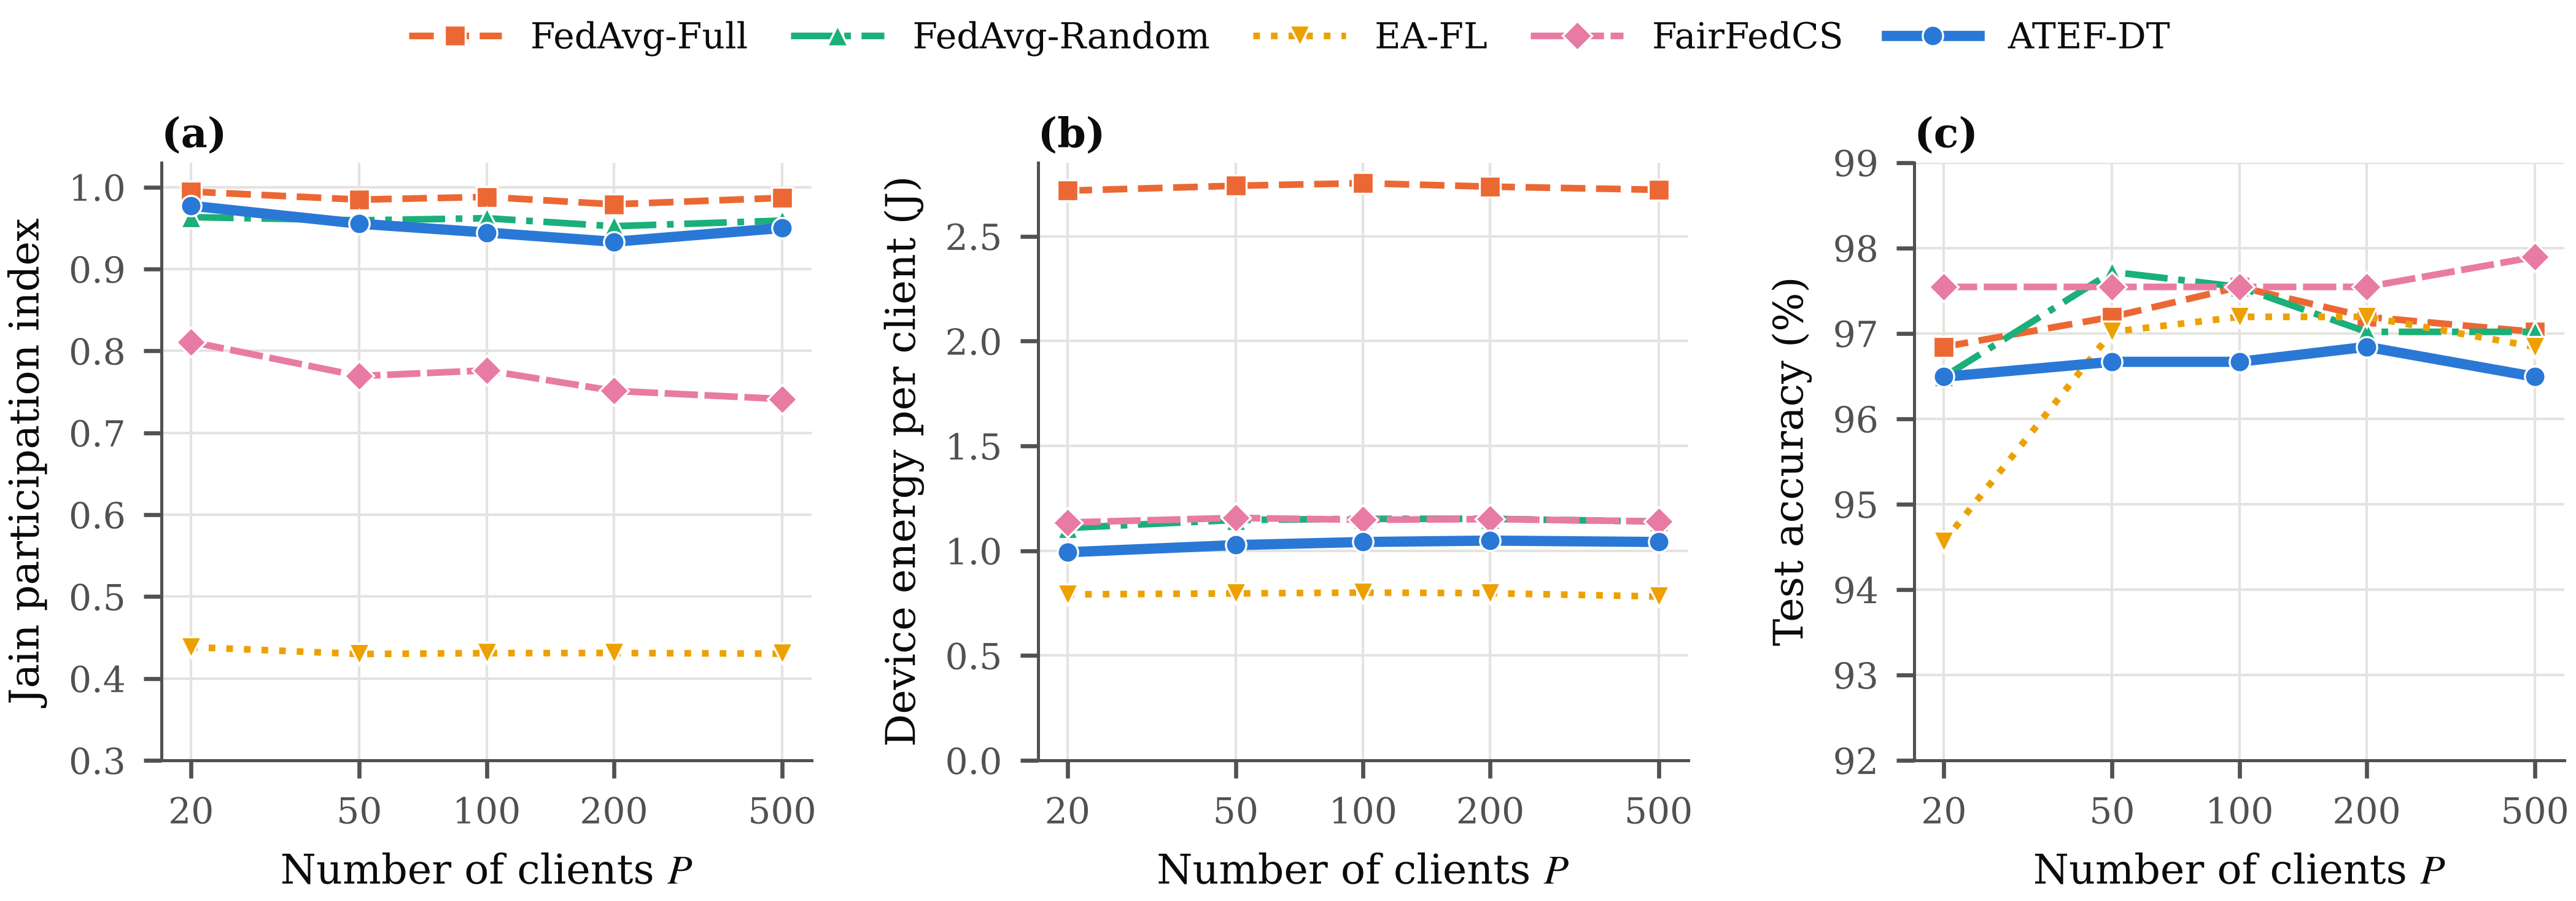
\includegraphics[width=\textwidth]{figures/fig_scalability}
	\revcap{R1.7(6)}{Scalability from 20 to \V{pmax} clients: (a)~Jain index, (b)~energy per client and (c)~test accuracy.}
	\label{fig:scalability}
\end{figure*}

\begin{table*}[t]
	\centering
	\revcap{E5}{Server-side time per round (ms).}
	\label{tab:overhead}
	\footnotesize
	\begin{tabular*}{\linewidth}{@{\extracolsep{\fill}}cccccccc}
		\toprule
		\textbf{Clients} & \textbf{Selected} & \textbf{Scoring and} & \textbf{Geometric} & \textbf{Weiszfeld} & \textbf{Reputation} & \textbf{Clipping and} & \textbf{Total} \\
		$\boldsymbol{P}$ & \textbf{per round} & \textbf{selection} & \textbf{median} & \textbf{iterations} & \textbf{update} & \textbf{aggregation} & \\
		\midrule
		\tabin{tab_overhead}
		\bottomrule
	\end{tabular*}
\end{table*}

\begin{figure*}[t]
	\centering
	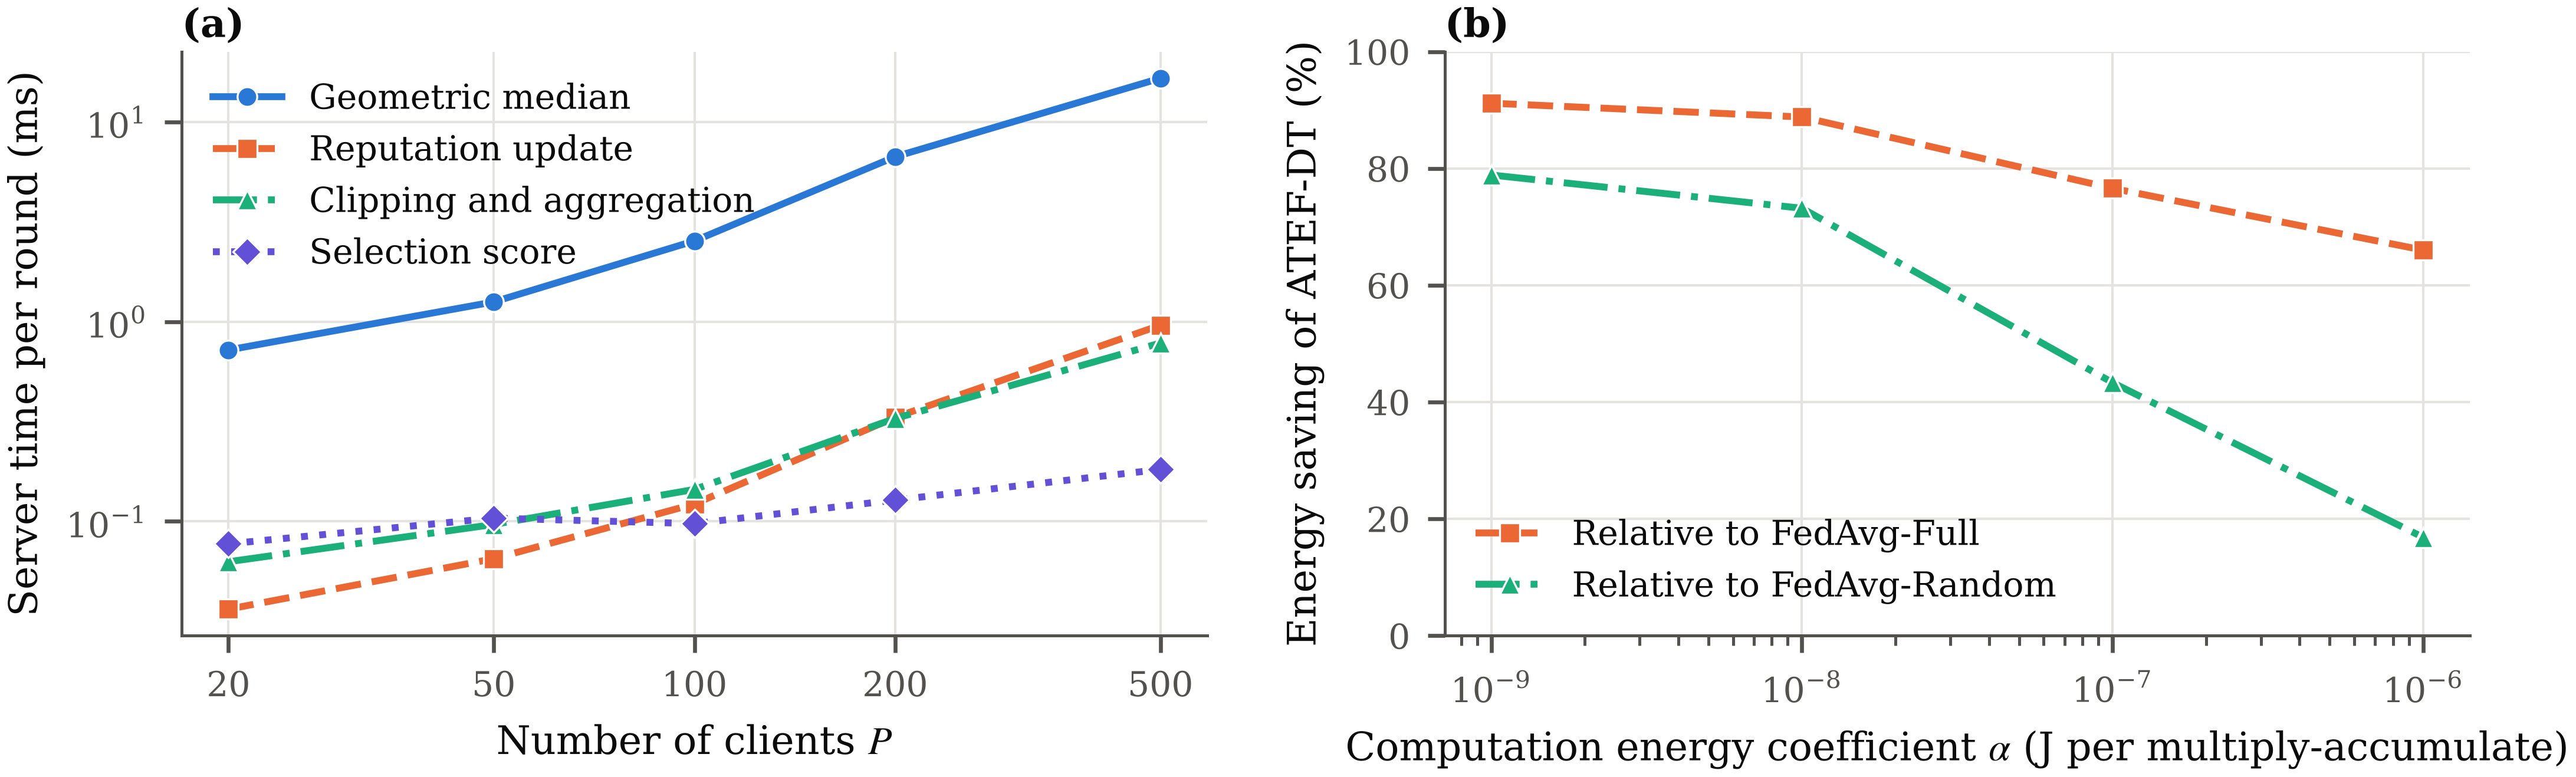
\includegraphics[width=\textwidth]{figures/fig_overhead}
	\revcap{R1.5, R2.5, R1.7(6)}{(a)~Server time per round and (b)~energy saving of ATEF-DT against the computation coefficient $\alpha$.}
	\label{fig:overhead}
\end{figure*}

\rtag{E5}\rev{Table~\ref{tab:overhead} reports the measured server time per round of the released single-threaded NumPy implementation.} The total grows from \V{t-total-20}~ms at 20 clients to \V{t-total-500}~ms at \V{pmax} clients and is dominated by the geometric median, which needs 10 to 15 Weiszfeld iterations; scoring and selection remain below a fifth of a millisecond. Figure~\ref{fig:overhead}(a) plots the components.

\subsection{Sensitivity to the Energy Parameters}
\label{subsec:sensitivity}
\rtag{R1.5, R2.5}\begin{revblock}Because the energy is computed from a model, its conclusions depend on the parameters of the model. Table~\ref{tab:alpha} and Figure~\ref{fig:overhead}(b) vary the computation coefficient $\alpha$ from $10^{-9}$ to $10^{-6}$~J. At the default, computation is \V{compshare-a6}\% of the energy of FedAvg-Full and the saving of ATEF-DT relative to FedAvg-Random is \V{sav-rand-a6}\%. As $\alpha$ decreases, communication dominates, quantization matters more, and the saving rises to \V{sav-rand-a8}\% at $10^{-8}$~J and \V{sav-rand-a9}\% at $10^{-9}$~J. The ranking of the methods also changes: for $\alpha\le 10^{-7}$~J, ATEF-DT consumes less than EA-FL, which transmits at full precision. The saving reported in Section~\ref{subsec:energyres} is therefore specific to a computation-dominated setting and is the smallest of those observed. Varying the amplifier efficiency $\eta_{\mathrm{PA}}$ between $0.2$ and $0.5$ changes the saving relative to FedAvg-Random only between \V{sav-rand-eta05}\% and \V{sav-rand-eta02}\%.\end{revblock}

\begin{table*}[t]
	\centering
	\revcap{R1.5, R2.5, E4}{Sensitivity to the computation energy coefficient $\alpha$.}
	\label{tab:alpha}
	\footnotesize
	\begin{tabular*}{\linewidth}{@{\extracolsep{\fill}}ccccccccc}
		\toprule
		 & \textbf{Computation} & \multicolumn{4}{c}{\textbf{Device energy (J)}} & \multicolumn{2}{c}{\textbf{Saving of ATEF-DT (\%)}} & \textbf{Jain index} \\
		\cmidrule(lr){3-6}\cmidrule(lr){7-8}
		$\boldsymbol{\alpha}$ \textbf{(J)} & \textbf{share (\%)} & \textbf{FedAvg-Full} & \textbf{FedAvg-Random} & \textbf{EA-FL} & \textbf{ATEF-DT} & \textbf{vs.\ Full} & \textbf{vs.\ Random} & \textbf{of ATEF-DT} \\
		\midrule
		\tabin{tab_alpha}
		\bottomrule
	\end{tabular*}
\end{table*}

\FloatBarrier
\subsection{Limitations}
\label{subsec:limitations}
\rtag{E7, E4, R1.5, R1.6, R1.7(3)}\begin{revblock}The energy, channel and twin environments are simulated rather than measured, the evaluation uses one small tabular data set, and the sensitivity of ATEF-DT is slightly below that of full participation. The reputation layer fails when adversaries form half of a selected set or collude, the score remains a heuristic for the long-run problem, and the framework provides data locality but no formal privacy guarantee.\end{revblock}

\section{Conclusion}
\label{sec:conclusion}
This article presented ATEF-DT, a framework that schedules battery-constrained clients of a federated digital-twin healthcare system with a single weighted-product score over predicted energy, participation and reputation, a twin-driven battery screen, per-client adaptive quantization and reputation-weighted aggregation. The score was formulated as a weighted-product scalarization with three proved properties, and a convergence bound was given for the update that is applied, with a bound on the participation bias in terms of the effective aggregation weights. On the WDBC data with simulated devices and channels, the framework matched the accuracy of full participation within the variation across seeds, used \V{sav-rand}\% less device energy than uniform sampling at the same budget, and reached a Jain participation index of \V{jain-atef}, against \V{jain-eafl} for energy-greedy selection. With 20\% label-flipping clients it retained \V{lf20-atef}\% accuracy. The comparison with alternative schedulers showed that the product rule is as efficient as tuned additive rules and, unlike them, insensitive to the scale of its criteria; the robustness study showed that the reputation layer protects through graded weights within a limited domain and fails outside it.

Future work will evaluate the framework on hardware and on longitudinal clinical data with demographic attributes, replace the within-round reference of the credibility engine by one that does not depend on the selected cohort, and combine the scheduler with client-level differential privacy under the constraint that selection is deterministic.

\section*{Declaration of generative AI and AI-assisted technologies}
\rtag{E6, R2.6}\rev{Figure~\ref{fig:architecture} is a schematic drawn by the authors in draw.io from boxes, arrows and typeset equations, and all result figures are produced by the released plotting script from the logged data; the manuscript contains no image produced by a generative model. During the preparation of this revision the authors used a large language model (Claude, Anthropic) to assist with the restructuring and language editing of the text, with the implementation of the simulation code and with the drawing of Figure~\ref{fig:architecture}. The authors reviewed and verified the resulting text, code and results, and take full responsibility for the content of the article.}


\appendix
\section{Properties of the Selection Score}
\label{app:score}
\begin{lemma}[Smallest values]
	\label{lem:topk}
	Let $v_p\in\mathbb{R}$ for $p$ in a finite set $\cF$ and let $1\le k\le|\cF|$. A set consisting of $k$ elements with the smallest values minimizes $\sum_{p\in\cS}v_p$ over all $\cS\subseteq\cF$ with $|\cS|=k$.
\end{lemma}
\begin{proof}
	Let $\cS$ consist of $k$ elements with the smallest values and let $\cS'$ be any other subset of size $k$. Pair each $p'\in\cS'\setminus\cS$ with a distinct $p\in\cS\setminus\cS'$; the two difference sets have the same size. Since $p\in\cS$ and $p'\notin\cS$, $v_p\le v_{p'}$. Summing over the pairs gives $\sum_{p\in\cS}v_p\le\sum_{p\in\cS'}v_p$.
\end{proof}

\begin{proof}[Proof of Proposition~\ref{prop:optimal}]
	(a)~Apply Lemma~\ref{lem:topk} with $v_p=\ln s_p^{(r)}=\lambda_E\ln\tilde e_p+\lambda_F\ln\tilde u_p+\lambda_T\ln\tilde t_p$. The logarithm is increasing, so the $k_r$ clients with the smallest scores are those with the smallest $v_p$, and the sum of the $v_p$ is the objective of~\eqref{eq:roundproblem}. (b)~Suppose $q\in\cF^{(r)}\setminus\cS^{(r)}$ dominates $p\in\cS^{(r)}$. All factors are positive and all exponents are positive, so $s_q^{(r)}<s_p^{(r)}$. But $p$ is selected and $q$ is not, which requires $s_p^{(r)}\le s_q^{(r)}$, a contradiction.
\end{proof}

\begin{proof}[Proof of Proposition~\ref{prop:pipeline}]
	Write $k=k_r$ and let all clients have the same reputation, so that the trust factor is a common constant. \emph{Energy first.} Let $\bar k$ clients have predicted energy $0$ and participation count $n$, and let $k$ further clients have predicted energy $e_1>0$ and participation count $0$. By~\eqref{eq:efactor} and~\eqref{eq:ufactor}, the first group has $\tilde e=\varepsilon_0$ and $\tilde u=1$, and the second has $\tilde e=e_1/(e_1+\varepsilon_0)+\varepsilon_0\le 1+\varepsilon_0$ and $\tilde u=1/(n+1)$. The pipeline keeps the first group and selects $k$ of its members. The ratio of the score of a member of the first group to that of a member of the second is at least $(\varepsilon_0/(1+\varepsilon_0))^{\lambda_E}(n+1)^{\lambda_F}$, which exceeds any $\theta>1$ for $n$ large enough; the second group is then the minimizer, and the product of the scores selected by the pipeline exceeds the minimum by more than $\theta^k\ge \theta$. \emph{Fairness first.} Let $k$ clients (group A) have count $0$ and the largest predicted energy, let $\bar k-k\ge 1$ clients (group B) have count $(n-1)/2$ for an odd $n$ and predicted energy $0$, and let at least one further client have count $n$. Then $\tilde u=1/(n+1)$ and $\tilde e\le 1+\varepsilon_0$ in group A, and $\tilde u=1/2$ and $\tilde e=\varepsilon_0$ in group B. The pipeline keeps groups A and B and then prefers group B, so it selects at least one member of group B. The ratio of the score of a member of group B to that of a member of group A is at least $(\varepsilon_0/(1+\varepsilon_0))^{\lambda_E}((n+1)/2)^{\lambda_F}$, which exceeds $\theta$ for $n$ large enough; group A is then the minimizer, and replacing one of its members by a member of group B multiplies the product by more than $\theta$.
\end{proof}

\begin{proof}[Proof of Proposition~\ref{prop:scale}]
	The transformation multiplies every score by the same constant $c_E^{\lambda_E}c_F^{\lambda_F}c_T^{\lambda_T}>0$ and therefore preserves their order. For the weighted sum, take two clients with $(\tilde e,\tilde u)=(0.2,1)$ and $(1,0.5)$, equal trust factors and $\lambda_E=\lambda_F=1$. The sums are $1.2$ and $1.5$, so the first client is preferred. With $c_E=0.1$ they become $1.02$ and $0.6$, and the second client is preferred. The products are $0.2$ and $0.5$ before the transformation and $0.02$ and $0.05$ after it; the first client is preferred in both cases.
\end{proof}

\section{Proof of Theorem~\ref{thm:convergence}}
\label{app:proofs}
\rtag{E3, R1.3, R2.3}\rev{By Assumption~\ref{ass:smooth} and~\eqref{eq:applied},
\begin{equation*}
	F(\w^{(r+1)})\le F(\w^{(r)})-\eta\,\langle\nabla F(\w^{(r)}),\g^{(r)}\rangle+\frac{L\eta^2}{2}\norm{\g^{(r)}}^2 .
\end{equation*}
Write $\nabla F$ for $\nabla F(\w^{(r)})$ and $\bar{\g}=\E_r[\g^{(r)}]=\bar s_r(\nabla F+\tilde{\bb}_r)$ with $\tilde{\bb}_r=\bb_r/\bar s_r$. Taking $\E_r$, using $\E_r\norm{\g^{(r)}}^2=\norm{\bar{\g}}^2+\E_r\norm{\g^{(r)}-\bar{\g}}^2\le\norm{\bar{\g}}^2+V$, and then $L\eta\le 1$ and $\bar s_r\le 1$, so that $L\eta^2\bar s_r^2\le\eta\,\bar s_r$,
\begin{align*}
	\E_r F(\w^{(r+1)})&\le F(\w^{(r)})-\eta\,\bar s_r\langle\nabla F,\nabla F+\tilde{\bb}_r\rangle\\
	&\quad+\frac{\eta\,\bar s_r}{2}\norm{\nabla F+\tilde{\bb}_r}^2+\frac{L\eta^2V}{2}\\
	&=F(\w^{(r)})-\frac{\eta\,\bar s_r}{2}\norm{\nabla F}^2+\frac{\eta\,\bar s_r}{2}\norm{\tilde{\bb}_r}^2+\frac{L\eta^2V}{2},
\end{align*}
where the equality expands the square. Since $\bar s_r\ge s_{\min}$ and $\bar s_r\norm{\tilde{\bb}_r}^2=\norm{\bb_r}^2/\bar s_r\le B^2/s_{\min}$ by Assumption~\ref{ass:update},
\begin{equation*}
	\frac{\eta\,s_{\min}}{2}\norm{\nabla F(\w^{(r)})}^2\le F(\w^{(r)})-\E_r F(\w^{(r+1)})+\frac{\eta B^2}{2s_{\min}}+\frac{L\eta^2V}{2}.
\end{equation*}
Taking the total expectation, summing over $r=0,\dots,R-1$, using $F(\w^{(R)})\ge F^{\star}$ and dividing by $\eta\,s_{\min}R/2$ gives~\eqref{eq:bound}.}

\section{Reproducibility}
\label{app:repro}
\rtag{E5, R2.7}\begin{revblock}The repository contains the package \texttt{atefdt} (data, model, system and energy model, quantizer, twin, selection rules, credibility engine, aggregation rules, attacks and the round-level simulator), the configuration file \texttt{configs/default.yaml} with the values of Table~\ref{tab:setup}, and three scripts. \texttt{experiments/run\_all.py} runs every experiment of Sections~\ref{sec:experiments} and~\ref{sec:results} and writes the results and the per-transmission logs; \texttt{experiments/make\_values.py} converts the results into the numbers and table bodies of this article; \texttt{experiments/make\_figures.py} draws Figures~\ref{fig:convergence}--\ref{fig:overhead}. No number in the article is typed by hand. A test suite checks the gradient of the model, the unbiasedness of the quantizer, Lemma~\ref{lem:rep}, Propositions~\ref{prop:optimal}--\ref{prop:scale} on random instances, the bound $s^{(r)}\ge\rho_{\min}/2$, the energy accounts, the determinism of the runs and the agreement of a fresh run with the stored results. The complete protocol runs in about three minutes on one processor core and requires only NumPy, SciPy, scikit-learn, Matplotlib and PyYAML; the versions used are recorded in the repository. Each seed fixes the partition, the initial model, the device parameters, the fading sequence and the adversaries through independent random streams, so a result can be reproduced exactly from its seed.\end{revblock}


\bibliographystyle{elsarticle-num}
\bibliography{references}
\end{document}
